\documentclass[a4paper,12pt]{article}

\usepackage{fontspec}
\usepackage{polyglossia}
\setmainlanguage{russian}
\setotherlanguage{english}

\setmainfont{Times New Roman}[Ligatures=TeX]
\newfontfamily\cyrillicfont{Times New Roman}[Ligatures=TeX]
\newfontfamily\cyrillicfonttt{Courier New}[Ligatures=TeX]

\usepackage{amsmath, amssymb, amsfonts, csquotes, array, geometry, textcomp, titlesec, listings, hyperref, caption, xcolor, import, subcaption}

\usepackage{pgffor}

% Numbering of only mentioned formulas
\usepackage{mathtools}
\mathtoolsset{showonlyrefs}

\usepackage{enumitem}
\usepackage{alphabeta} % Optional: for Greek if needed

\makeatletter
\AddEnumerateCounter{\asbuk}{\russian@asbuk@alph}{щ} % section 8.1
\makeatother

% Define Cyrillic enumeration using custom labels
\setlist[enumerate, 1]{label=\asbuk*)}
\renewcommand{\thesubfigure}{\asbuk{subfigure}} % Используем кириллицу вместо латиницы

% Changing itemize dots to dashes
\setlist[itemize]{label=-}

\usepackage{graphicx}
\graphicspath{{images/}}  % Presets the "images" directory

\usepackage[backend=biber, style=numeric-comp, sorting=none]{biblatex}
\addbibresource{references.bib} % Файл со списком литературы

% Для управления таблицами и правильной нумерации
\usepackage{caption}            % Настройка подписей
\captionsetup[table]{justification=raggedright, labelsep=period, textfont=normalsize}

% Для изменения шрифта в таблицах
\usepackage{array}

% Для многострочных заголовков и гибкой ширины колонок
\usepackage{makecell}
\renewcommand\theadfont{\bfseries}

% Patch caption to store the number only
\makeatletter
\newcommand{\TableNumberRight}{
  \refstepcounter{table}% increment and make labelable
  \noindent\hfill\textbf{Таблица \thetable}
}
\makeatother

\usepackage{etoolbox}
\AtBeginEnvironment{tabular}{\small}  % or \footnotesize, \scriptsize

\usepackage{siunitx}
\sisetup{
  group-separator     = {\,},   % optional: use space between thousands
  detect-all,                 % makes font/style match surroundings
  table-align-text-post = false
}

\geometry{left=25mm,right=20mm,top=25mm,bottom=25mm}

\hypersetup{
  unicode=true,       % Поддержка Unicode (важно для русского языка)
  pdfauthor={Ваше Имя}, % Автор документа
  pdftitle={Название документа}, % Заголовок PDF
  pdfkeywords={ключевые слова}, % Ключевые слова
  pdfstartview=FitH,  % Открытие PDF в ширину страницы
  % colorlinks=true,    % Цветные ссылки
  % linkcolor=blue,     % Цвет ссылок
  % citecolor=red,      % Цвет ссылок на цитаты
  % filecolor=magenta,  % Цвет ссылок на файлы
  % urlcolor=cyan       % Цвет ссылок на URL
	linkbordercolor = white,          
	citebordercolor = green,
}
\renewcommand{\figureautorefname}{Рис.}
\renewcommand{\tableautorefname}{Табл.}
\renewcommand{\equationautorefname}{Уравнение}
\renewcommand{\sectionautorefname}{Раздел}
\renewcommand{\subsectionautorefname}{Подраздел}
\renewcommand{\subsubsectionautorefname}{Подраздел}

\setcounter{page}{2}

\title{\Huge{Предсказание вязкости жидкостей с помощью методов машинного обучения на основе параметров уравнения состояния}}
\author{Панов Михаил Федорович \\ Руководитель: Писарев Василий Вячеславович}
\date{Москва --- 2025}

\begin{document}

% Титульный лист
\maketitle
\thispagestyle{empty}
\newpage

% Задание на ВКР
\section*{Задание на ВКР}
(Текст задания на ВКР)

% Аннотация
\section*{Аннотация}
(Аннотация на русском языке)

% Abstract
\section*{Abstract}
(Аннотация на английском языке)
\newpage

% Содержание
\tableofcontents
\newpage

% Введение
\section*{Введение}
\addcontentsline{toc}{section}{Введение}
(Введение: актуальность, цель, задачи, объект, структура)

% Глава 1
\section{Обзор литературы и постановка задачи}
  \subsection{Свойства вязкости и ее роль в инженерных задачах}

    \subsubsection{Вязкость в промышленных приложениях}

Вязкость -- ключевой реологический параметр, определяющий сопротивление жидкости деформации при сдвиге. Ее значение напрямую влияет на гидродинамические характеристики систем, включая распределение давления, скорости потока и теплопередачу. В ряде инженерных процессов, таких как транспортировка нефти и газа, проектирование теплообменников, химическая переработка и производство смазочных материалов, точное знание вязкости определяет эффективность и безопасность эксплуатации оборудования. 

В многофазных или сложных многокомпонентных системах, например, в синтетических нефтяных смесях, вязкость влияет на фазовое поведение, устойчивость эмульсий и общую производительность процессов. В микрофлюидике и фармацевтике контроль вязкости необходим для предсказуемого управления потоками и дозированием веществ.

    \subsubsection{Значение точного прогнозирования вязкости}

Точное моделирование вязкости представляет собой одну из ключевых задач в термодинамическом моделировании жидкостей. На практике невозможно измерить вязкость для всех возможных условий и составов, особенно в системах, содержащих десятки или сотни компонентов, как, например, в нефтяной промышленности. В таких случаях используются предсказательные модели, основанные на молекулярных или термодинамических представлениях, которые позволяют получить значения вязкости при отсутствии экспериментальных данных.

Среди современных подходов особое внимание уделяется моделям, связывающим вязкость с остаточной энтропией и другими термодинамическими величинами, так как они обеспечивают высокую переносимость и физическую обоснованность. Связь между вязкостью и избыточной энтропией подмечали во многих работах, например \cite{taib2020residual}. Особенно актуальны такие модели для расчетов в широком диапазоне температур и давлений, а также при переходе к сверхкритическим и конденсированным фазам.

Таким образом, разработка универсальных моделей вязкости, не требующих индивидуальной подгонки параметров, является приоритетной задачей в области физико-химического моделирования сложных жидкостей.

  \subsection{Обзор подходов к предсказанию вязкости}

    \subsubsection{Ограничения эмпирических формул}
      Большинство классических подходов к описанию вязкости основаны на эмпирических уравнениях, содержащих подобранные коэффициенты для конкретных веществ или их классов. Такие модели, как правило, работают в узком диапазоне температур и давлений и требуют предварительных измерений вязкости. Это делает их трудноприменимыми для новых или редких веществ, особенно в условиях, когда экспериментальные данные недоступны или ограничены. (for example)

    \subsubsection{Модель MYS}

      Одной из наиболее универсальных и известных современных моделей для описания динамической вязкости жидкостей в широком диапазоне условий является модель, предложенная Ильей Полищуком в 2015 году -- так называемая \textit{Modified Yarranton–Satyro (MYS)} модель~\cite{polishuk2015viscosity}. Ее основное назначение -- обеспечить точное предсказание вязкости для широкого спектра органических жидкостей, включая углеводороды, в диапазонах температур от тройной точки до высоких значений, а также при изменяющемся давлении.

      \textbf{Предпосылки модели.}  
      Изначально модель Yarranton–Satyro (YS) создавалась для описания вязкости как функции плотности, температуры и параметров молекулярного строения. Polishuk модифицировал ее, чтобы избежать необходимости экспериментальной подгонки и позволить использовать только параметры, выводимые из уравнений состояния (в частности, SAFT). Основной целью стало создание аналитической корреляции, не требующей знания вязкости как входного параметра, но использующей только предсказуемые или известные характеристики вещества.
      
      \textbf{Структура модели.}  
      Модель MYS представляет собой сложную аналитическую формулу, включающую молекулярные параметры, полученные из теории SAFT:
      
      \begin{equation}
        \eta = 0.1 \left( \exp \left( \frac{c_1 \sqrt{m} + \ln \left( 1 + \frac{M_w^4}{c_2 v^4 m^3} \right) \ln \left( \frac{T}{T_{\text{tp}} + 120} \right)}{
        \exp \left( \frac{1.04 v}{N_{\text{av}} m \sigma^3} \exp \left( \frac{c_3 P}{\varepsilon_k \sqrt{-\frac{dP}{dv} \cdot \sqrt{m v}}} \right) - 1 \right) - 1} 
        \right) - 1 \right) + \eta_0
        \label{eq:mys}
      \end{equation}
      
      где:  
      \begin{itemize}
        \item $\eta$ -- динамическая вязкость (Па·с)
        \item $\eta_0$ -- вязкость идеального газа (обычно берется как постоянная или ноль)
        \item $m$ -- молярная масса
        \item $M_w$ -- молекулярная масса
        \item $v$ -- мольный объем
        \item $T$ -- температура
        \item $T_{\text{tp}}$ -- температура тройной точки
        \item $P$ -- давление
        \item $\varepsilon_k$ -- параметр межмолекулярного взаимодействия
        \item $dP/dv$ -- производная давления по объему (рассчитанная из уравнения состояния)
        \item $\sigma$ -- эффективный диаметр молекулы
        \item $N_{\text{av}}$ -- число Авогадро
        \item $c_1=0.27$, $c_2=2.5*10^{11}$, $c_3=2.1$ -- эмпирические коэффициенты (подобраны автором)
      \end{itemize}
      
      \textbf{Особенности модели.}  
      - Формула MYS не требует априорного знания вязкости, но использует величины, производные из термодинамических функций, так как она связана с параметрами уравнения состояния CP-PC-SAFT.
      - Автор демонстрирует среднюю ошибку модели на уровне менее 10\% для широкой выборки жидкостей.
      - Подход особенно эффективен для органических и углеводородных жидкостей.
      
      \textbf{Применение в данной работе.}  
      Модель MYS была выбрана в качестве основного ориентира для сравнения, поскольку:
      \begin{itemize}
        \item Она является одной из наиболее точных универсальных формул, не требующих подбора индивидуальных коэффициентов для каждого вещества.
        \item Она опирается на термодинамически интерпретируемые параметры, аналогично нашему подходу.
        \item Ее точность считается приемлемой для инженерных и прикладных задач.
        \item Она сохраняет свою точность на достаточно большом диапазоне давлений и температур
      \end{itemize}
      
      В настоящем исследовании модели машинного обучения и символьной регрессии сравниваются по точности предсказания вязкости с моделью MYS. Наши модели демонстрируют в ряде случаев ошибку до 2\% -- значительно ниже, чем у MYS -- что позволяет рассматривать их как более точную альтернативу в условиях, когда имеются данные для обучения модели.
      
    \subsubsection{Уравнение состояния CP-PC-SAFT}
    
    Основное уравнение состояния PC-SAFT выражается через вклад свободной энергии Гельмгольца \( a \):
    
    \begin{equation}
    A(v, T) = A^{\text{id}} + A^{\text{hs}} + A^{\text{chain}} + A^{\text{disp}} + A^{\text{assoc}}
    \end{equation}
    
    Где:
    \begin{itemize}
        \item \( A^{\text{id}} \) -- вклад идеального газа;
        \item \( A^{\text{hs}} \) -- вклад жестких сфер;
          \[
          A^{HS} = RT \frac{m}{\zeta_0} \left( \frac{3 \zeta_1 \zeta_2}{1 - \zeta_3} + \frac{\zeta_2^3}{\zeta_3 (1 - \zeta_3)^2} \right) + \left( \frac{\zeta_2^3}{\zeta_3^2} - \zeta_0 \right) \ln [1 - \zeta_3] \sqrt{\frac{d^3 (\zeta_3 - 1)}{\zeta_3 \sigma^3 - d^3}}
          \]
        \item \( A^{\text{chain}} \) -- вклад цепных взаимодействий;
          \[
          A^{chain} = RT \sum_i x_i x_j (1 - m_{ij}) \ln [g_{ij} (d_{ij})]^{hs}
          \]
        \item \( A^{\text{disp}} \) -- вклад дисперсионных сил;
          \begin{align}
          A^{\text{disp}} = -RN_{\text{Av}} \Bigg( & \frac{2 \pi (\varepsilon / k) m^2 \sigma^3}{\nu} I_1 \notag \\
          & + \frac{\pi (\varepsilon / k)^2 m^3 \sigma^3}{\nu T \left(
          1 + \frac{m (8 \zeta_3 - 2 \zeta_3^2)}{(1 - \zeta_3)^4} +
          \frac{(1 - m)(20 \zeta_3 - 27 \zeta_3^2 + 12 \zeta_3^3 - 2 \zeta_3^4)}{((1 - \zeta_3)(2 - \zeta_3))^2}
          \right)} I_2 \Bigg)
          \end{align}
    
        \item \( A^{\text{assoc}} \) -- вклад ассоциативных взаимодействий.
        \item $d$ -- эффективный диаметр молекулы, связанный с $\sigma$ через $\theta$.
          \[
            d = \theta * \sigma
          \]
        \item $\sigma$ -- характерный размер молекулы (диаметр сферического сегмента). В случае смеси нескольких веществ:
          \begin{equation}
            \sigma = \sqrt[3]{\frac{\sum_i x_i x_j m_i m_j \sigma_{ij}^3}{(\sum_i x_i m_{ii})^2}}
          \end{equation}
        \item $\theta$ -- коэффициент масштабирования длины связи.
          \[
          \theta = \frac{1 + 0.2977 (k / \varepsilon) T}{1 + 0.33163 (k / \varepsilon) T + 0.0010477 (k / \varepsilon)^2 T^2}
          \]
        \item $\zeta_k$ -- параметр упаковки молекул.
          \[
          \zeta_k = \frac{\pi N_{av}}{6 \nu} \sum_i x_i m_i \sigma_i^{dk}
          \]
        \item $\varepsilon / k_B$ -- приведенная энергия взаимодействия между частицами. В случае смеси нескольких веществ:
          \begin{equation}
            \varepsilon / k = \frac{\sum_i x_i x_j m_i m_j \sigma_{ij}^3 (\varepsilon / k)_{ij}}{\sigma^3 (\sum_i x_i m_{ii})^2}
          \end{equation}
        \item $k_B$ -- постоянная Больцмана;
        \item $N_{Av}$ -- число Авогадро.
        \item $m$ -- количество сегментов в молекуле. В случае смеси нескольких веществ:
          \begin{equation}
            m = \sum_i x_i m_i
          \end{equation}
        \item $x_i$ -- мольная доля компонента $i$.
        \item $P$ -- давление.
        \item $T$ -- температура.
        \item $v$ -- мольный объем.
        \item $d_{ij}$ -- средний эффективный диаметр молекул $i$ и $j$.
        \item $g_{ij}$ -- функция радиальной корреляции молекул $i$ и $j$.
          \begin{equation}
            g_{ij}(d_{ij})^{hs} = \frac{1}{1 - \zeta_3} + \frac{3d_{i}d_{j}\zeta_2}{(d_{ii} + d_{jj})(1 - \zeta_3)^2} + 2 \left( \frac{d_{i}d_{j}}{d_{ii} + d_{jj}} \right)^2 \frac{\zeta_2^2}{(1 - \zeta_3)^3}
          \end{equation}
        \item $\nu$ -- молярный объем системы.
        \item $I_1$, $I_2$ -- интегралы в дисперсионном вкладе.
        \item $(\varepsilon / k)_{ij}$ -- приведенная энергия взаимодействия между разными компонентами $i$ и $j$. 
          \begin{equation}
              (\varepsilon / k)_{ij} = (1 - k_{ij}) \sqrt{(\varepsilon / k)_{ii} (\varepsilon / k)_{jj}}
          \end{equation}
        \item $m_{ij}$ -- эффективное среднее число сегментов при взаимодействии компонентов $i$ и $j$:
          \[
            m_{ij} = \left(1 - l_{ij}\right) \frac{m_{ii} + m_{jj}}{2}
          \]
        \item $\sigma_{ij}$ -- характерный средний диаметр сегментов при взаимодействии компонентов $i$ и $j$, рассчитанный как простое среднее арифметическое:
          \[
            \sigma_{ij} = \frac{\sigma_{ii} + \sigma_{jj}}{2}
          \]
        \item $k_{ij}$, $l_{ij}$ -- коэффициент парного взаимодействия и параметр согласования размеров сегментов. Считаются равными нулю, либо подбираются на основании экспериментальных данных.
    
    \end{itemize}
    
    \subsubsection{Параметры веществ  в CP-PC-SAFT}

В рамках CP-PC-SAFT каждое вещество описывается тремя основными параметрами:
\begin{itemize}
    \item \( m \) -- число сегментов в молекуле;
    \item \( \sigma \) -- эффективный диаметр сегмента молекулы;
    \item \( \varepsilon \) -- энергия взаимодействия между сегментами.
\end{itemize}

Эти параметры определяются через критическую точку и температуру кипения вещества, а не через эмпирическую подгонку, что делает модель более универсальной.

В модели CP-PC-SAFT параметры вещества корректируются так, чтобы соответствовать следующим условиям \cite{polishuk2014standardized}:

\begin{equation}
\left( \frac{\partial P}{\partial v} \right)_{T_c} = 0, \quad
\left( \frac{\partial^2 P}{\partial v^2} \right)_{T_c} = 0
\end{equation}

\begin{equation}
P_c = P_{\text{c, exp}}
\end{equation}

\begin{equation}
\rho_{\text{liq, triple}} = \rho_{\text{liq, triple, exp}}
\end{equation}

Здесь:
\begin{itemize}
    \item \( P_c \) -- давление в критической точке;
    \item \( T_c \) -- критическая температура;
    \item \( \rho_{\text{liq, triple}} \) -- жидкостная плотность в тройной точке.
\end{itemize}

Условиями для поиска параметров являются критическая температура, критическое давление и плотность жидкости при температуре плавления, соответствующие экспериментальным значениям. Необходимость знания значений всего трех экспериментальных величин для вычисления всех параметров вещества делает модель CP-PC-SAFT крайне привлекательной в вопросах предсказания свойств новых веществ и смесей на большом диапазоне условий. 

\subsubsection{Трудности машинного обучения}

Применение методов машинного обучения (ML) к задачам физико-химического моделирования, включая предсказание вязкости жидкостей, в последние годы стало популярным направлением (for example). Такие методы, как правило, позволяют автоматически выявлять сложные зависимости в данных и достигать высокой точности без необходимости ручного выбора аналитических формул. Тем не менее, несмотря на прогресс в области ML, существует ряд фундаментальных причин, по которым машинное обучение нельзя считать универсальным решением (панацеей) для предсказания реологических свойств веществ.

\textbf{1. Ограниченная интерпретируемость моделей.}
Большинство моделей машинного обучения, включая градиентный бустинг, нейронные сети и случайные леса, представляют собой черные ящики, в которых интерпретация внутренней логики и значимости отдельных признаков затруднена. Это особенно критично в контексте задач молекулярной термодинамики, где важна не только точность, но и возможность объяснить результат через физически обоснованные параметры. В противоположность этому, аналитические формулы, такие как MYS, или, потенциально, символьная регрессия (используемая в данной работе) позволяют сохранять интерпретируемость и анализировать вклад каждой переменной.

\textbf{2. Риск переобучения и проблемы обобщения.}
Как показано в ходе данной работы, даже простые модели, такие как линейная регрессия или случайный лес, демонстрируют высокий риск переобучения при специальном разбиении выборки. В частности, точность существенно снижается при валидации на новых веществах, не представленных в обучающей выборке. Особенно ярко это проявляется в случае веществ, отличающихся по агрегатному состоянию -- например, бутана. Это указывает на ограниченную способность моделей ML к интерполяции за пределами обучающих данных.

\textbf{3. Зависимость от качества и полноты данных.}
Модели машинного обучения требуют большого количества однородных и хорошо размеченных данных. В случае термодинамических величин, таких как вязкость, часто доступны только ограниченные экспериментальные измерения, сделанные в различающихся условиях и с неоднородной точностью. Это может как ограничивать возможности ML, делая необходимым использование большего количества уникальных производных признаков, полученных, например, из уравнений состояния, так и приводить к переобучению из-за попыток модели подстроиться к условиям конкретного эксперимента.

\textbf{4. Отсутствие устойчивости к физическим границам.}
Некоторые модели ML могут выдавать предсказания, нарушающие физические ограничения -- например, отрицательную вязкость или аномальные значения при экстремальных температурах и давлениях. Это особенно заметно в моделях, не обученных на таких данных. В отличие от этого, аналитические формулы и интерпретируемые модели могут быть сконструированы с учетом физических асимптотик и ограничений.

\textbf{5. Практические требования к применению.}
Для внедрения моделей в инженерную практику важны не только высокая точность, но и компактность, воспроизводимость и простота вычислений. Модели машинного обучения, особенно глубокие нейросети, могут быть ресурсоемкими и плохо воспроизводимыми. Символьные формулы или регрессии, напротив, могут быть легко реализованы даже в простых инженерных расчетах.

Таким образом, несмотря на мощность и гибкость современных методов машинного обучения, они должны использоваться с осторожностью, особенно в задачах с физико-химическим контекстом. Наиболее перспективным направлением видится интеграция ML с физически обоснованными подходами -- в частности

\subsubsection{Символьная регрессия}

Символьная регрессия (symbolic regression, SR) -- это подход к построению моделей, при котором алгоритм не просто находит численные параметры в заданной структуре формулы как в линейной регрессии, а ищет саму структуру уравнения, наиболее точно описывающего зависимость между входными и выходными переменными. В отличие от традиционных методов машинного обучения, символьная регрессия формирует аналитическое выражение в виде комбинаций математических операций и входных признаков.

\textbf{Мотивация применения.}
Основным преимуществом SR является высокая интерпретируемость получаемых моделей. Вместо подбора большого количества слабоинтерпретируемых коэффициентов, как в случае с нейросетями, модель находит короткие выражения, состоящие из качественно различающихся блоков (операторов). Каждое уравнение, сформированное таким способом, может быть проанализировано, сопоставлено с физическими законами, а также непосредственно использовано в инженерных расчетах. Это особенно важно при работе с термодинамическими и молекулярными свойствами, где значение имеет не только точность, но и физический смысл модели.

В рамках настоящего исследования SR использовалась для поиска наиболее компактных и точных выражений, связывающих вязкость с параметрами уравнения состояния CP-PC-SAFT и производными термодинамическими величинами, включая мольный объем, избыточную энтропию и производную давления по объему.

\textbf{Используемый инструмент: PySR.}
Для реализации символьной регрессии применялась современная библиотека PySR (Python Symbolic Regression) \cite{cranmer2023pysr}. Эта библиотека сочетает возможности языка Python для настройки задач и быстродействие языка Julia, где реализована основная эволюционная оптимизация. PySR использует алгоритмы на основе генетического программирования, направленные на поиск выражений с оптимальным компромиссом между точностью и сложностью.

Основные особенности PySR:
\begin{itemize}
  \item Многофункциональная система операторов: поддерживаются стандартные математические функции (логарифм, экспонента, степень и др.).
  \item Поддержка многоцелевой оптимизации: минимизация ошибки при контроле за длиной формулы.
  \item Устойчивость к переобучению: регуляризация сложности встроена в процесс поиска.
  \item Высокая производительность благодаря параллельному выполнению на CPU и GPU.
\end{itemize}

\textbf{Результаты применения.}
В ходе экспериментов символьная регрессия позволила получить компактные формулы с ошибкой, сравнимой с ошибкой модели MYS. Таким образом, символьная регрессия показала себя как перспективный инструмент, позволяющий извлекать простые закономерности. Ее применение может дополнить использование других моделей и усилить акцент на физическую обоснованность результатов.

  \subsection{Цель и задачи исследования}

    \subsubsection{Цель исследования}
    
    Разработка метода прогнозирования вязкости жидкостей на основе параметров уравнения состояния CP-PC-SAFT с точностью, превосходящей существующую модель MYS.
    
    \subsubsection{Задачи исследования}
    
    Для реализации постасленной цели были намечены следующие задачи:
    
    \begin{enumerate}
      \item \textbf{Сбор и подготовка экспериментальных данных}{
        \begin{itemize}
          \item Получение доступа к данным термодинамических параметров веществ.
          \item Формирование базы данных свойств жидкостей и газов на основе ThermoML.
          \item Фильтрация выборки для получения только интересующих веществ с замеренными температурой, давлением и вязкостью.
          \item Предварительная обработка данных для приведения интересующих параметров к единому формату.
        \end{itemize}
      }
    
        \item \textbf{Расчет производных параметров}
        \begin{itemize}
            \item Вычисление мольного объема по известным температуре и давлению.
            \item Определение избыточной энтропии $s^{\text{ex}}$ по известным мольному объему и температуру через производную избыточной энергии Гельмгольца по температуре.
            \item Вычисление вязкости идеального газа.
        \end{itemize}
    
        \item \textbf{Генерация и отбор новых признаков, проверка их значимости}
        \begin{itemize}
            \item Создание производных признаков, отражающих физические закономерности вязкости.
            \item Оценка их статистической значимости для модели, и отбор наиболее полезных.
            \item Валидация роли различных признаков в прогнозировании вязкости, в том числе избыточной энтропии.
        \end{itemize}
    
        \item \textbf{Обучение, сравнение и оптимизация моделей машинного обучения}
        \begin{itemize}
            \item Построение и проверка эффективности различных моделей ML, таких как линейная регрессия, градиентный бустинг, случайный лес и нейросетевые методы.
            \item Оптимизация гиперпараметров для повышения точности наиболее перспективных моделей.
            \item Использование символьной регрессии (PySR) для поиска интерпретируемых аналитических зависимостей.
        \end{itemize}
    
        \item \textbf{Сравнение разработанной модели с существующей моделью MYS}
        \begin{itemize}
            \item Оценка точности предложенного метода на тестовых данных.
            \item Анализ преимуществ и недостатков разработанных моделей по сравнению с MYS.
            \item Формирование рекомендаций по дальнейшему развитию метода прогнозирования вязкости жидкостей.
        \end{itemize}
    \end{enumerate}
  
  \subsection{Выводы по главе}
В первой главе был проведен обзор современных представлений о вязкости как важном термодинамическом параметре и существующих подходах к ее моделированию. Показано, что вязкость оказывает существенное влияние на поведение жидких и многофазных систем в различных инженерных приложениях -- от нефтепереработки до микрофлюидики.

Рассмотрены эмпирические формулы, применяемые для расчета вязкости, а также универсальные аналитические модели, такие как MYS (Modified Yarranton–Satyro). Несмотря на широкую применимость первых, они имеют ограничения в точности при отсутствии экспериментальных данных для подгонки или при переходе к новым веществам. В свою очередь, MYS не всегда дает достаточные для прикладных задач оценки ввиду своей универсальности.  

Особое внимание было уделено уравнению состояния CP-PC-SAFT, которое позволяет получить необходимые параметры вещества без тщательной подгонки, опираясь лишь на критические и тройные точки. Это делает его особенно подходящим для предсказательных моделей, работающих на широком спектре условий и веществ, таких как MYS или разрабатываемая в рамках данной работы.

Кроме того, рассмотрены возможности машинного обучения и его ограничения в задачах физико-химического моделирования, включая проблемы интерпретируемости, переобучения и нарушения физических ограничений. На этом фоне была обоснована целесообразность использования символьной регрессии и системы генерации новых признаков как методов, сочетающих гибкость ML с интерпретируемостью и физической обоснованностью аналитических формул.

Таким образом, глава обосновывает научную и практическую значимость задачи предсказания вязкости на основе параметров уравнения состояния и подтверждает пользу разработки нового подхода, сочетающего машинное обучение и следование физическим принципам. Далее в работе рассматривается реализация этого подхода на практике.

\newpage

% Глава 2
\section{Сбор и обработка данных}
  \subsection{Работа с базой данных}
    \subsubsection{Источник данных: база ThermoML}
    
      Для получения экспериментальных данных о вязкости в данной работе использовалась база данных \textbf{ThermoML}, разработанная Национальным институтом стандартов и технологий США (NIST). ThermoML представляет собой машиночитаемый формат на основе XML, предназначенный для хранения и распространения термодинамических и физико-химических данных, включая фазовые равновесия, плотности, давления, температуры и вязкости чистых веществ и смесей.
      
      Одной из ключевых особенностей ThermoML является строго стандартизированная структура описания данных, что позволяет автоматизировать их извлечение и минимизировать необходимость ручной предобработки. Это особенно важно при формировании выборок для задач машинного обучения, где требуется согласованность единиц измерения и форматов.
      
    \subsubsection{ThermoPyL для чтения данных}
      Для взаимодействия с базой ThermoML была использована специализированная Python-библиотека \textbf{ThermoPyL}. Данная библиотека предоставляет инструменты для:
      \begin{itemize}
        \item автоматического чтения и парсинга XML-файлов ThermoML;
        \item фильтрации данных по фазе и составу;
        \item преобразования данных в формат \texttt{pandas.DataFrame} для последующей обработки в Python;
        \item агрегации данных по условиям экспериментов;
        \item экспорта результатов в формат CSV.
      \end{itemize}
      
      Использование библиотеки \texttt{ThermoPyL} позволило автоматизировать процесс подготовки данных, не углубляясь в анализ и обработку XML файлов из ThermoML.
    
  \subsection{Выбор веществ и критерии включения}
  
  Для анализа были выбраны чистые вещества, относящиеся к классу насыщенных углеводородов. Они обладают простой молекулярной структурой и широко используются в промышленности, что делает их удобным объектом для моделирования. Основным критерием отбора было наличие значительного объема экспериментальных данных по вязкости в базе ThermoML. В финальную выборку вошли восемь веществ:
    \begin{itemize}
      \item Бутан: получено 311 экспериментальных точек из 2 работ \cite{acs.jced.5b00654,s10765-006-0053-2}
      \item Пентан: получено 50 экспериментальных точек из 3 работ \cite{acs.jced.7b00650,j.jct.2005.10.011,je0501944}
      \item Гексан: получено 127 экспериментальных точек из 25 работ \cite{acs.jced.5b00152,acs.jced.8b00589,j.fluid.2013.07.060,j.fluid.2018.08.001,j.jct.2004.09.021,j.jct.2005.03.024,j.jct.2005.07.008,j.jct.2005.10.011,j.jct.2007.05.016,j.jct.2008.02.005,j.tca.2005.10.008,je020114l,je020131a,je030107c,je034002l,je049576k,je049777o,je060389r,je060491o,je800048f,je8006138,je9006597,s10765-005-5572-8,s10765-006-0053-2,s10765-009-0622-2}
      \item Гептан: получено 443 экспериментальных точек из 28 работ \cite{acs.jced.5b00152,acs.jced.7b00121,j.fluid.2006.01.030,j.fluid.2010.10.009,j.fluid.2016.11.029,j.jct.2004.09.021,j.jct.2005.03.024,j.jct.2005.10.011,j.jct.2006.01.012,j.jct.2013.09.017,j.jct.2015.12.021,j.tca.2005.10.008,j.tca.2015.08.005,j.tca.2018.10.018,je020131a,je049662k,je049776w,je049777o,je400835u,je5007532,je600554h,je700202h,je8003707,je9006597,je900969u,s10765-009-0667-2,s10765-012-1373-z,s10765-014-1759-1}
      \item Октан: получено 362 экспериментальных точек из 32 работ \cite{acs.jced.6b00391,acs.jced.7b00121,acs.jced.7b00650,j.fluid.2010.10.009,j.jct.2003.12.005,j.jct.2004.09.021,j.jct.2005.03.024,j.jct.2005.10.011,j.jct.2006.01.012,j.jct.2007.05.016,j.jct.2008.02.005,j.jct.2013.09.017,j.jct.2014.09.015,j.tca.2005.10.008,j.tca.2015.08.005,je020131a,je034017j,je034208m,je049572f,je049776w,je0503296,je060389r,je300899n,je4004806,je400835u,je600554h,je800348s,je800417q,je9006597,s10765-006-0053-2,s10765-008-0542-6,s10765-014-1759-1}
      \item Нонан: получено 115 экспериментальных точек из 13 работ \cite{acs.jced.7b00121,acs.jced.7b00650,j.fluid.2010.10.009,j.jct.2004.09.021,j.jct.2005.03.024,j.jct.2005.10.011,j.jct.2013.09.017,je200757a,je300899n,je400250u,je400835u,je700202h,je700428f}
      \item Декан: получено 224 экспериментальных точек из 25 работ \cite{acs.jced.5b00270,acs.jced.6b00542,acs.jced.7b00121,acs.jced.7b00650,j.fluid.2010.10.009,j.jct.2003.12.005,j.jct.2004.09.021,j.jct.2005.03.024,j.jct.2005.10.011,j.jct.2007.05.016,j.jct.2008.02.005,j.jct.2013.05.014,j.jct.2013.09.017,je034208m,je0501585,je060389r,je300899n,je400250u,je400835u,je4008926,je800348s,je800417q,je800635g,s10765-005-5572-8,s10765-008-0542-6}
      \item Додекан: получено 412 экспериментальных точек из 25 работ \cite{acs.jced.6b00391,acs.jced.6b00542,acs.jced.6b00688,acs.jced.7b00201,acs.jced.7b00466,acs.jced.7b00650,acs.jced.7b00866,acs.jced.8b00008,acs.jced.8b00438,acs.jced.8b01135,acs.jced.8b01233,acs.jced.9b00187,j.fluid.2015.07.022,j.jct.2003.12.005,j.jct.2004.09.021,j.jct.2005.03.024,j.jct.2013.12.022,j.jct.2014.02.012,j.jct.2015.12.021,je034208m,je060491o,je200757a,je400493x,je400835u,je5000132}
    \end{itemize}
    
    Для включения записи в выборку требовалось наличие всех трех параметров:
    \begin{itemize}
      \item температуры (\( T \), К),
      \item давления (\( P \), Па),
      \item вязкости (\( \eta \), Па·с).
    \end{itemize}
    
    Записи, в которых отсутствовала хотя бы одна из этих величин, исключались. Дополнительная фильтрация по фазе не производилась, поскольку, например, для бутана полезны данные как в жидкой, так и в газообразной фазе. Каждая выборка сохранялась в виде отдельного CSV-файла для дальнейшей обработки. В результате было собрано более 2000 уникальных записей.

  \subsection{Распределение экспериментальных данных}
    \subsubsection{Фазовое состояние}
      Большая часть данных принадлежала к жидкой фазе. Только 295 точек для бутана находятся в состоянии газа. Так как модель MYS расчитана на данные как в жидкой, так и в газовой фазе, было решено оставить точки, принадлежащие газовой фазе, несмотря на то, что они представлены только бутаном.

    \subsubsection{Температура}
      Значения температуры итоговых данных распределены следующим образом \autoref{fig:data_distribution_temperature}:
      
      \begin{itemize}
          \item \textbf{Минимальная температура}: \(273.15\) К
          \item \textbf{Максимальная температура}: \(693.7\) К
          \item \textbf{Среднее значение температуры}: \(406\) К
          \item \textbf{Медианное значение температуры}: \(403\) К
          \item \textbf{Явный пик в районе}: \(300\) К
      \end{itemize}
      
      \begin{figure}[ht!]
          \centering
          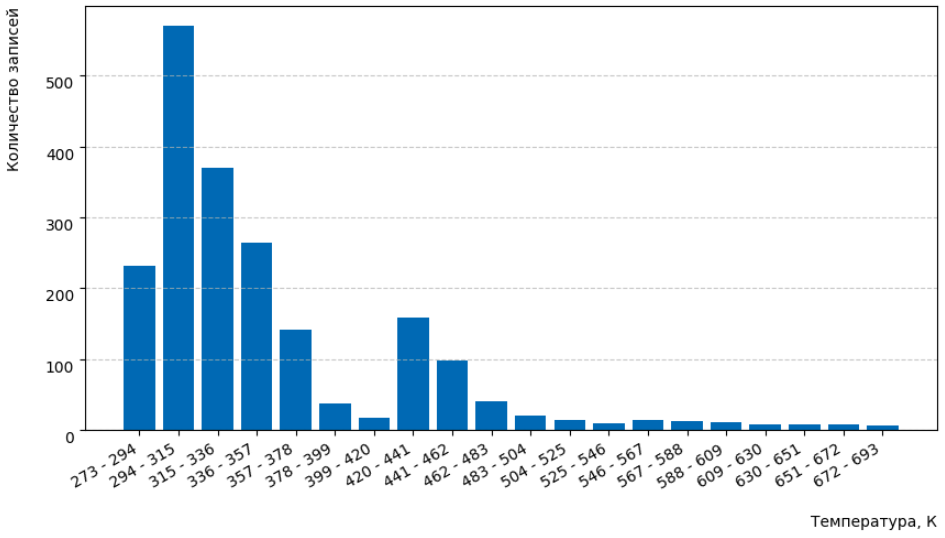
\includegraphics[width=0.8\textwidth]{data_distribution_temperature.png}
          \caption{Распределение температуры в экспериментальных данных}
          \label{fig:data_distribution_temperature}
      \end{figure}

    \subsubsection{Давление}
    Значения давления итоговых данных распределены следующим образом \autoref{fig:data_distribution_pressure}:

      \begin{itemize}
          \item \textbf{Минимальное давление}: \(57.183\) кПа
          \item \textbf{Максимальное давление}: \(245.16\) МПа
          \item \textbf{Среднее значение давления}: \(23\) МПа
          \item \textbf{Медианное значение давления}: \(6\) МПа
          \item \textbf{Резкий пик наблюдается в районе}: \(1\) атмосферы
      \end{itemize}

      Данные удобнее отображать в логарифмической шкале, так как в ней они относительно равномерно распределены.
      \begin{figure}[ht!]
        \centering
        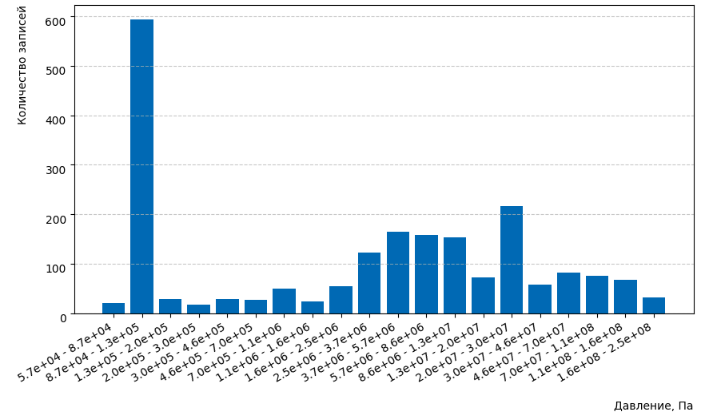
\includegraphics[width=0.8\textwidth]{data_distribution_pressure.png}
        \caption{Распределение давления в экспериментальных данных (логарифмическая шкала по горизонтали)}
        \label{fig:data_distribution_pressure}
      \end{figure}

    \subsubsection{Вязкость}
      Значения вязкости итоговых данных распределены следующим образом \autoref{fig:data_distribution_viscosity}:
      
      \begin{itemize}
          \item \textbf{Минимальная вязкость}: \(7.3\) мкПа\(\cdot\)с
          \item \textbf{Максимальная вязкость}: \(5.8\) мПа\(\cdot\)с
          \item \textbf{Среднее значение вязкости}: \(500\) мкПа\(\cdot\)с
          \item \textbf{Медианное значение вязкости}: \(385\) мкПа\(\cdot\)с
          \item \textbf{Небольшой пик наблюдается в районе}: \(10\) мкПа\(\cdot\)с (эксперименты с бутаном)
      \end{itemize}
      
      Распределение вязкости, аналогично распределению давления, удобнее отображать в логарифмическом масштабе.
      
      \begin{figure}[ht!]
          \centering
          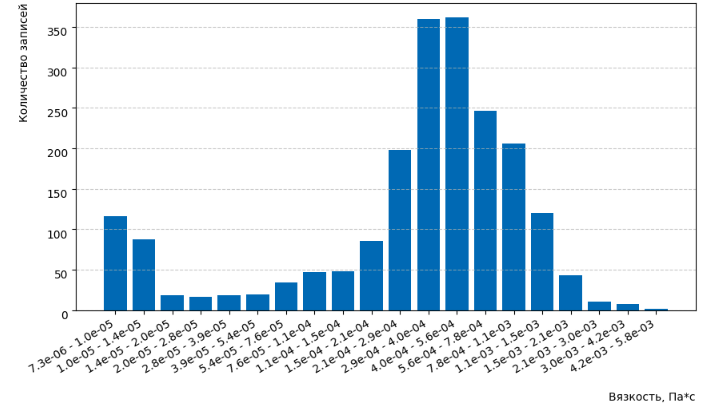
\includegraphics[width=0.8\textwidth]{data_distribution_viscosity.png}
          \caption{Распределение вязкости в экспериментальных данных (логарифмическая шкала по горизонтали)}
          \label{fig:data_distribution_viscosity}
      \end{figure}

  \subsection{Добавление параметров уравнения CP-PC-SAFT}
    Как уже было упомянуто выше, у каждого вещества есть единственный набор параметров для уравнения CP-PC-SAFT: $\sigma$, $\delta$, $\varepsilon/k_b$ и $m$. Для всех исследуемых веществ данные признаки были добавлены в датасет. Эти параметры представляют собой ключевые свойства каждого соединения, поскольку их можно точно определить, что позволяет назвать их основными характеристиками.
    \begin{table}[ht]
      \TableNumberRight

      \begin{center}
        \textbf{Основные характеристики компонентов}
        \vspace*{\fill}
      \end{center}

      \vspace{0.8ex}
      
      % Table aligned left + full width
      \noindent
      \begin{tabular}{|l|S|S|S|S|S|}
        \hline
        \textbf{Вещество} & \textbf{Молярная масса, (г/моль)} & \textbf{m} & \textbf{$\varepsilon/k_b$, K} & \textbf{\sigma, \si{\angstrom} } & \textbf{\delta} \\
        \hline
        бутан & 58.120 & 2.48262 & 209.446 & 3.65040 & 1.15976 \\
        пентан & 72.150 & 3.06424 & 212.528 & 3.62421 & 1.16385 \\
        гексан & 86.180 & 3.51081 & 218.238 & 3.65575 & 1.16091 \\
        гептан & 100.210 & 4.07032 & 220.494 & 3.63515 & 1.16631 \\
        октан & 114.230 & 4.45475 & 225.287 & 3.67868 & 1.17934 \\
        нонан & 128.257 & 4.85100 & 229.271 & 3.70469 & 1.18722 \\
        декан & 142.284 & 5.27013 & 232.262 & 3.72188 & 1.20260 \\
        додекан & 170.338 & 6.01209 & 238.240 & 3.76983 & 1.22522 \\
        \hline
      \end{tabular}
      \label{tab:components_data}
    \end{table}

  \subsection{Вычисление производных величин}
    В ходе работы возникала потребность в дополнении данных новыми величинами, которые можно вычислить используя уже известные величины. Это нужно как для увеличения количества признаков, которыми могли бы пользоваться модели машинного обучения, так и для возможности пользоваться некоторыми формулами.
    
    \subsubsection{Вязкость идеального газа}
      Вязкость идеального газа является одним из параметров уравнения MYS~\eqref{eq:mys}. Можно было бы опустить этот коэффициент и использовать вместо него ноль, и формально формула осталась бы вполне точной для жидкой фазы. Однако для газовой области именно этот коэффициент дает наибольший вклад. Пренебречь им -- значит закрыть глаза на половину картины. Поэтому было решено вычислить вязкость идеального газа для всех экспериментальных точек, чтобы обеспечить максимальную точность модели в целом. Поскольку уравнение MYS служит основным критерием точности, задача вычисления $\eta_0$ приобрела особую значимость.

      Для расчета вязкости идеального газа использовался классический подход на основе параметров Леннарда--Джонса -- $(\varepsilon/k)_{LJ}$ и $\sigma_{LJ}$, которые были определены по температуре плавления и мольному объему вещества. Этот подход, несмотря на свою простоту, оказывается весьма работоспособным при корректной выборке входных данных. Температура плавления ($T_m$) и плотность в жидком состоянии ($\rho$) использовались для расчета мольного объема $v$ по формуле:
      \[
      v = \frac{M}{\rho},
      \]
      где $M$ -- молярная масса.
      
      Далее параметры $\varepsilon/k$ и $\sigma$ определялись следующим образом:
      \[
        (\varepsilon/k)_{LJ} = 1.92 \cdot T_m, \quad 
        \sigma_{LJ} = \left( \frac{2.3 \cdot v}{\pi N_A \cdot 2/3} \right)^{1/3},
      \]
      где $N_A$ -- число Авогадро. Стоит отметить, что здесь $v$ переводился в кубические метры, а итоговое значение $\sigma$ -- в ангстремы.
     
      \begin{table}[ht]
        \TableNumberRight
      
        \begin{center}
          \textbf{Параметры Леннарда--Джонса для выбранных алканов}
          \vspace*{\fill}
        \end{center}
      
        \vspace{0.8ex}
      
        \noindent
        \begin{tabular}{|l
                |S[round-mode=places,round-precision=2]
                |S[round-mode=places,round-precision=4]|}

          \hline
          \textbf{Вещество} & {\textbf{$(\varepsilon/k_b)_{LJ}$, K}} & {\textbf{$\sigma_{LJ}$, \si{\angstrom}}} \\
          \hline
          бутан   & 410.00 & 4.9970 \\
          пентан  & 345.00 & 5.7690 \\
          гексан  & 413.00 & 5.9090 \\
          гептан  & 350.59 & 6.4406 \\
          октан   & 345.00 & 5.7690 \\
          нонан   & 413.00 & 5.9090 \\
          декан   & 467.52 & 7.0836 \\
          додекан & 506.11 & 7.4540 \\
          \hline
        \end{tabular}
        \label{tab:lj_params}
      \end{table}

      Параметры Леннард–Джонса для бутана, пентана, гексана, гептана, октана и нонана были взяты из справочника по вязкости газовых смесей \cite{голубев2013вязкость}. Параметры для декана и додекана были ввычисленны на основании температуры тройной точки и плотности при нормальных условиях с помощью формулы из той же книги. Коэффициенты для одного и того же вещества могут разниться в зависимости от интервала температур, в котором они были вычислены. При этом отмечается, что при расчетах ошибка, допущенная в определении величины $(\varepsilon/k_b)_{LJ}$, дает значительно меньшую ошибку в определении величины вязкости. 

      Указанные величины использовались для расчета вязкости идеального газа. Формула основана на кинетической теории газов и включает поправку на столкновения. Ее можно найти в продвинутой литературе по молекулярной динамике \cite{голубев2013вязкость}. Итоговое выражение имеет вид:
      \[
        \eta_0 = \frac{5}{16} \cdot \frac{\sqrt{MRT}}{\pi^{1/2} \cdot \sigma_{LJ}^2 \cdot \Omega(T^*) \cdot N_A},
      \]
      где $T^*$ -- приведенная температура, а $\Omega$ -- коэффициент столкновений, зависящий от $T^*$:
      \[
        T^* = \frac{RT}{(\varepsilon/k_b)_{LJ}}, \quad
      \Omega(T^*) = \frac{A}{(T^*)^B} + C e^{-D T^*} + E e^{-F T^*} + R T^{*B} \sin(S T^{*W} - P).
      \]
      Ниже приведены значения эмпирических коэффициентов, использованных в выражении для функции столкновений $\Omega(T^*)$. Эти значения были взяты из работы \cite{neufeld1972collision} и использованы без модификации.
      \begin{table}[ht]
        \TableNumberRight
        \begin{center}
          \textbf{Коэффициенты для расчета функции столкновений $\Omega(T^*)$}
          \vspace*{\fill}
        \end{center}
      
        \vspace{0.8ex}
        \noindent
        \begin{tabular}{|c|S|}
          \hline
          \textbf{Коэффициент} & {\textbf{Значение}} \\
          \hline
          $A$ & 1.16145 \\
          $B$ & 0.14874 \\
          $C$ & 0.52487 \\
          $D$ & 0.77320 \\
          $E$ & 2.16178 \\
          $F$ & 2.43787 \\
          $R$ & -0.0006435 \\
          $S$ & 18.0323 \\
          $W$ & -0.76830 \\
          $P$ & 7.27371 \\
          \hline
        \end{tabular}
        \label{tab:neufeld_coeffs}
      \end{table}
      
      Расчеты выполнялись для каждой строки из экспериментальной выборки с помощью функции `apply()` библиотеки `pandas`. Итоговая вязкость $\eta_0$ вносилась в результирующий CSV-файл, на основе которого строилось дальнейшее сравнение с экспериментальными и модельными данными.      
      
      Рапределение вычисленной вязкости имеет следующие свойства:

      \begin{itemize}
          \item \textbf{Минимальная вязкость}: \(4.913 \times 10^{-6}\) Па\(\cdot\)с
          \item \textbf{Максимальная вязкость}: \(1.653 \times 10^{-5}\) Па\(\cdot\)с
          \item \textbf{Среднее значение}: \(8.711 \times 10^{-6}\) Па\(\cdot\)с
          \item \textbf{Медианное значение}: \(8.602 \times 10^{-6}\) Па\(\cdot\)с
      \end{itemize}
      
      Распределение вязкости имеет максимальную частоту значений вокруг \(7.1 \times 10^{-6}\) Па\(\cdot\)с.
      Отмечаются пики около \(6.1 \times 10^{-6}\) Па\(\cdot\)с и \(1.2 \times 10^{-5}\) Па\(\cdot\)с, что указывает на неравномерное распределение вязкости.
      
      \begin{figure}[ht!]
          \centering
          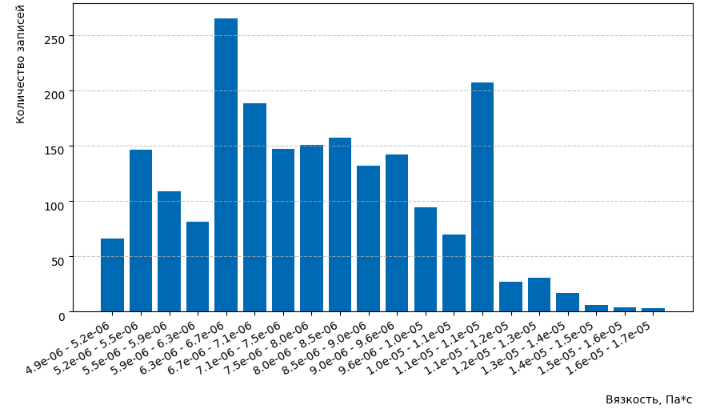
\includegraphics[width=0.8\textwidth]{data_distribution_viscosity_ideal_gas.png}
          \caption{Распределение вязкости идеального газа в экспериментальных данных (логарифмическая шкала по горизонтали)}
          \label{fig:data_distribution_viscosity_ideal_gas}
      \end{figure}

    \subsubsection{Мольный объем}
     
      Мольный объем \( v \) является одной из трех ключевых переменных уравнения состояния SAFT наряду с температурой \( T \) и давлением \( P \). Однако, чтобы получить энергию системы в явном виде, можно обойтись без давления. Тем не менее, в большинстве экспериментальных данных давление указано, а плотность -- нет, поэтому мольный объем приходится восстанавливать численно.
      
      Пусть задана точка с известными температурой \( T \) и давлением \( P \). Зная аналитическое выражение для энергии системы \( A(T, v) \), можно вычислить давление как производную:
      
      \[
      P = -\left( \frac{\partial A}{\partial v} \right)_T
      \]
      
      Тогда задача нахождения мольного объема \( v \) сводится к решению уравнения:
      
      \[
      P(v, T) = P_{\text{эксп}}
      \]
      
      Решение этой задачи проводится численно, например, методом половинного деления или методом Ньютона. При этом важно дополнительно проверить, что производная давления по объему отрицательна:
      
      \[
      \left( \frac{\partial P}{\partial v} \right)_T < 0
      \]
      
      Это необходимо для физической осмысленности и устойчивости найденного состояния.
      
      На практике был реализован алгоритм, основанный на бинарном поиске в заданном диапазоне объемов. Для каждой экспериментальной точки из базы данных была рассчитана пара: мольный объем \( v \) и производная давления по объему при данной температуре. Алгоритм корректно отработал на всех точках: он всегда находил первое значение объема, при котором давление совпадает с заданным и производная отрицательна.
      Для всех вычислений использовался язык программирования Julia и реализация уравнения состояния в библиотеке $CP\_PC\_SAFT$ \cite{cppcsaft2024}.
      Распределение вычисленного мольного объема имеет следующие свойства:

      \begin{itemize}
          \item \textbf{Минимальный мольный объем}: \(8.940 \times 10^{-5}\) м\(^3\)/моль
          \item \textbf{Максимальный мольный объем}: \(5.703 \times 10^{-2}\) м\(^3\)/моль
          \item \textbf{Среднее значение мольного объема}: \(4.700 \times 10^{-4}\) м\(^3\)/моль
          \item \textbf{Медианное значение мольного объема}: \(1.721 \times 10^{-4}\) м\(^3\)/моль
          \item \textbf{Главный пик наблюдается в районе медианного значения} 
      \end{itemize}
      
      На гистограмме распределение мольного объема представлено в логарифмическом масштабе \autoref{fig:data_distribution_molar_volume}.
      
      \begin{figure}[ht!]
          \centering
          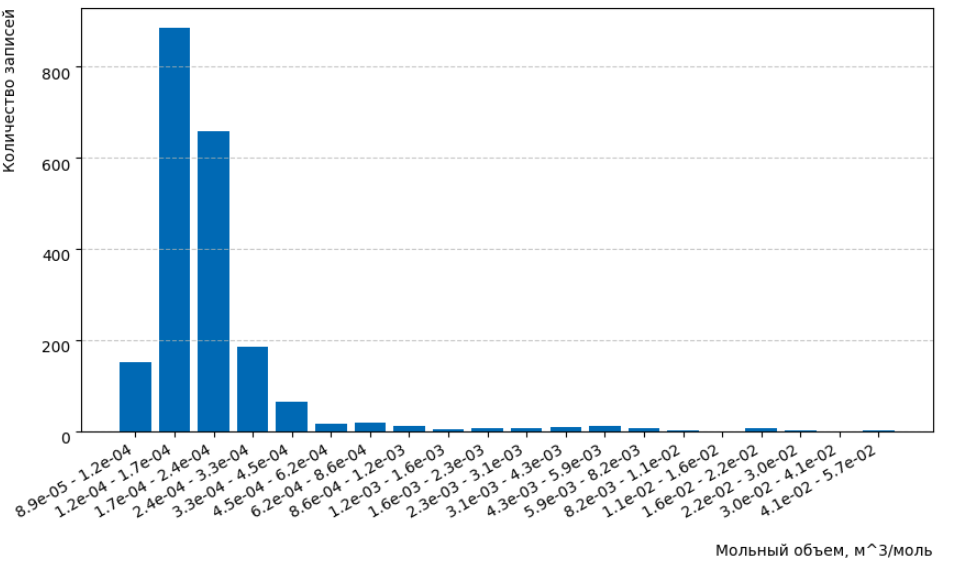
\includegraphics[width=0.8\textwidth]{data_distribution_molar_volume.png}
          \caption{Распределение мольного объема в экспериментальных данных (логарифмическая шкала)}
          \label{fig:data_distribution_molar_volume}
      \end{figure}

    \subsubsection{Избыточная энтропия}

      Избыточная энтропия -- важная термодинамическая характеристика, определяемая как производная избыточной свободной энергии Гельмгольца по температуре со знаком минус.

      Избыточная энергия представляется в виде полной энергии без вклада идеального газа $A^{\text{id}}$:
      
      \begin{equation}
      A^{\text{res}}(v, T) = A^{\text{hs}} + A^{\text{chain}} + A^{\text{disp}},
      \end{equation}
      
      Тогда избыточная мольная энтропия принимает вид:
      \begin{equation}
      s^{\text{res}}(v, T) = - \left( \frac{\partial A^{\text{res}}}{\partial T} \right)_v.
      \end{equation}
      
      В работе \cite{roknia2020entropy} было высказано предположение, согласно которому логарифм безразмерной вязкости жидкости можно аппроксимировать полиномом от нормированной избыточной энтропии:
      
      \begin{equation}
      \ln(\eta^*) = A + B s^* + C (s^*)^2 + D (s^*)^3,
      \end{equation}
      
      где нормированная избыточная энтропия определяется как:
      
      \begin{equation}
      s^* = \frac{s^{\text{res}}(v, T)}{m k_B}.
      \end{equation}
      
      Здесь:
      
      \begin{itemize}
        \item $A^{\text{res}}$ -- избыточная свободная энергия Гельмгольца (участвует в первых двух уравнениях);
        \item $\eta_0$ -- характеристическая (референсная) вязкость;
        \item $\eta^* = \eta / \eta_0$ -- безразмерная вязкость;
        \item $A$, $B$, $C$, $D$ -- эмпирические параметры, определяемые регрессией.
      \end{itemize}

      Основываясь на этом, можно сказать, что избыточная энтропия является важным признаком для предсказания вязкости. Разумно ожидать, что модели машинного обучения будут активно применять данные значения для улучшения результата.

      Для расчета избыточной энтропии использовалась библиотека \texttt{CP\_PC\_SAFT} на языке Julia для вычисления уравнения CP-PC-SAFT, а также другие библиотеки.

      Распределение вычисленной величины имеет следующие свойства:

      \begin{itemize}
          \item \textbf{Минимальное значение}: \(-1.295 \times 10^{2}\)
          \item \textbf{Максимальное значение}: \(-4.671 \times 10^{-2}\)
          \item \textbf{Среднее значение}: \(-6.291 \times 10^{1}\)
          \item \textbf{Медианное значение}: \(-6.740 \times 10^{1}\)
      \end{itemize}
      
      Распределение имеет максимальную частоту значений вокруг \(-5.8 \times 10^{1}\). Отмечаются пики около \(-7.1 \times 10^{1}\) и \(-4.5 \times 10^{1}\), что может указывать на неравномерное распределение величины.
      
      \begin{figure}[ht!]
          \centering
          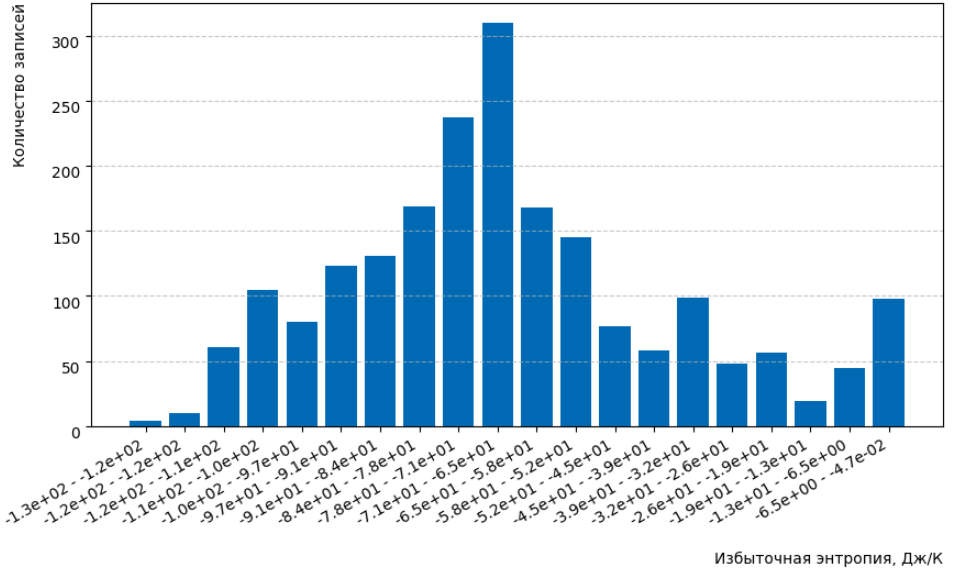
\includegraphics[width=0.8\textwidth]{data_distribution_excess_entropy.png}
          \caption{Распределение вычисленной избыточной энтропии}
          \label{fig:data_distribution_excess_entropy}
      \end{figure}
      
  \subsection{Выводы по главе}
    В данной главе был описан процесс сбора и предварительной обработки экспериментальных данных о вязкости для насыщенных углеводородов с использованием базы ThermoML и библиотеки ThermoPyL. Отбор и агрегация данных производились с учетом полноты необходимых параметров (температура, давление, вязкость). Основной акцент был сделан на чистые вещества, так как анализ данных систем проще, а количество экспериментов больше, чем для смесей.

    Анализ распределений показал, что явных выбросов, артефактов или дубликатов в собранных данных не наблюдается. Однако гораздо более существенную проблему представляет собой смещение распределения в сторону типичных условий, таких как область около 300 Кельвинов или 1 атмосферы. Это, вероятно, связано с предпочтениями экспериментаторов и ограничениями лабораторной аппаратуры. Подобные смещения могут повлиять на обобщающую способность моделей, особенно в предсказании вне хорошо охваченных областей параметров.

    Таким образом, несмотря на общее высокое качество данных и их стандартизированный формат, уже на этапе сбора можно отметить наличие неравномерности, которую важно учитывать при последующем анализе и обучении моделей.
\newpage

% Глава 3
\section{Интерпретируемые модели и генерация признаков}

  Одной из ключевых задач настоящей работы является не только получение точных предсказаний вязкости, но и выявление физически осмысленных закономерностей. Для этого был проведён анализ интерпретируемых моделей -- от теоретически обоснованной модели MYS до автоматически полученных выражений с помощью символьной регрессии. Наряду с этим была разработана система генерации новых признаков, направленная на улучшение точности моделей и выявление скрытых зависимостей в данных.

  \subsection{Модель MYS}

    Первой была проанализирована основная в данной работе модель для сравнения с новыми моделями — MYS (Modified Yarranton–Satyro).
    
    Для оценки точности ее предсказаний были использованы следующие метрики:
    
    \begin{itemize}
      \item \textbf{RMSE (корень из среднеквадратичной ошибки)}:
      \begin{equation}
        \mathrm{RMSE} = \sqrt{\frac{1}{n} \sum_{i=1}^{n} \left( \eta_i^{\text{model}} - \eta_i^{\text{exp}} \right)^2}
      \end{equation}
      где \( \eta_i^{\text{model}} \) — значение вязкости, предсказанное моделью, \( \eta_i^{\text{exp}} \) — экспериментальное значение, \( n \) — общее число точек.
    
      \item \textbf{Среднее относительное отклонение}:
      \begin{equation}
        \mathrm{MeanRelativeError} = \frac{1}{n} \sum_{i=1}^{n} \left| \frac{\eta_i^{\text{model}} - \eta_i^{\text{exp}}}{\eta_i^{\text{exp}}} \right|
      \end{equation}

      \item \textbf{Среднее абсолютное отклонение}:
      \begin{equation}
        \mathrm{MeanAbsoluteError} = \frac{1}{n} \sum_{i=1}^{n} \left| \eta_i^{\text{model}} - \eta_i^{\text{exp}} \right|
      \end{equation}
    \end{itemize}
    
    \medskip
    
   Для оценки эффективности модели использованы две метрики выше: среднее относительное отклонение и среднее абсолютное отклонение. Бутан представлен в основном точками газовой фазы, у которых значения вязкости занчительно ниже, чем у остальных данных и маленькая абсолютная ошибка порождает очень большую относительную. Поэтому бутан был исключен из рассмотрения, так как график относительной ошибки становится абсолютно неинформативным. На \autoref{fig:mys_rmse} и \autoref{fig:mys_relative_error} представлены графики этих двух метрик, иллюстрирующих поведение модели MYS на экспериментальных данныx:  

    \begin{figure}[ht!]
        \centering
        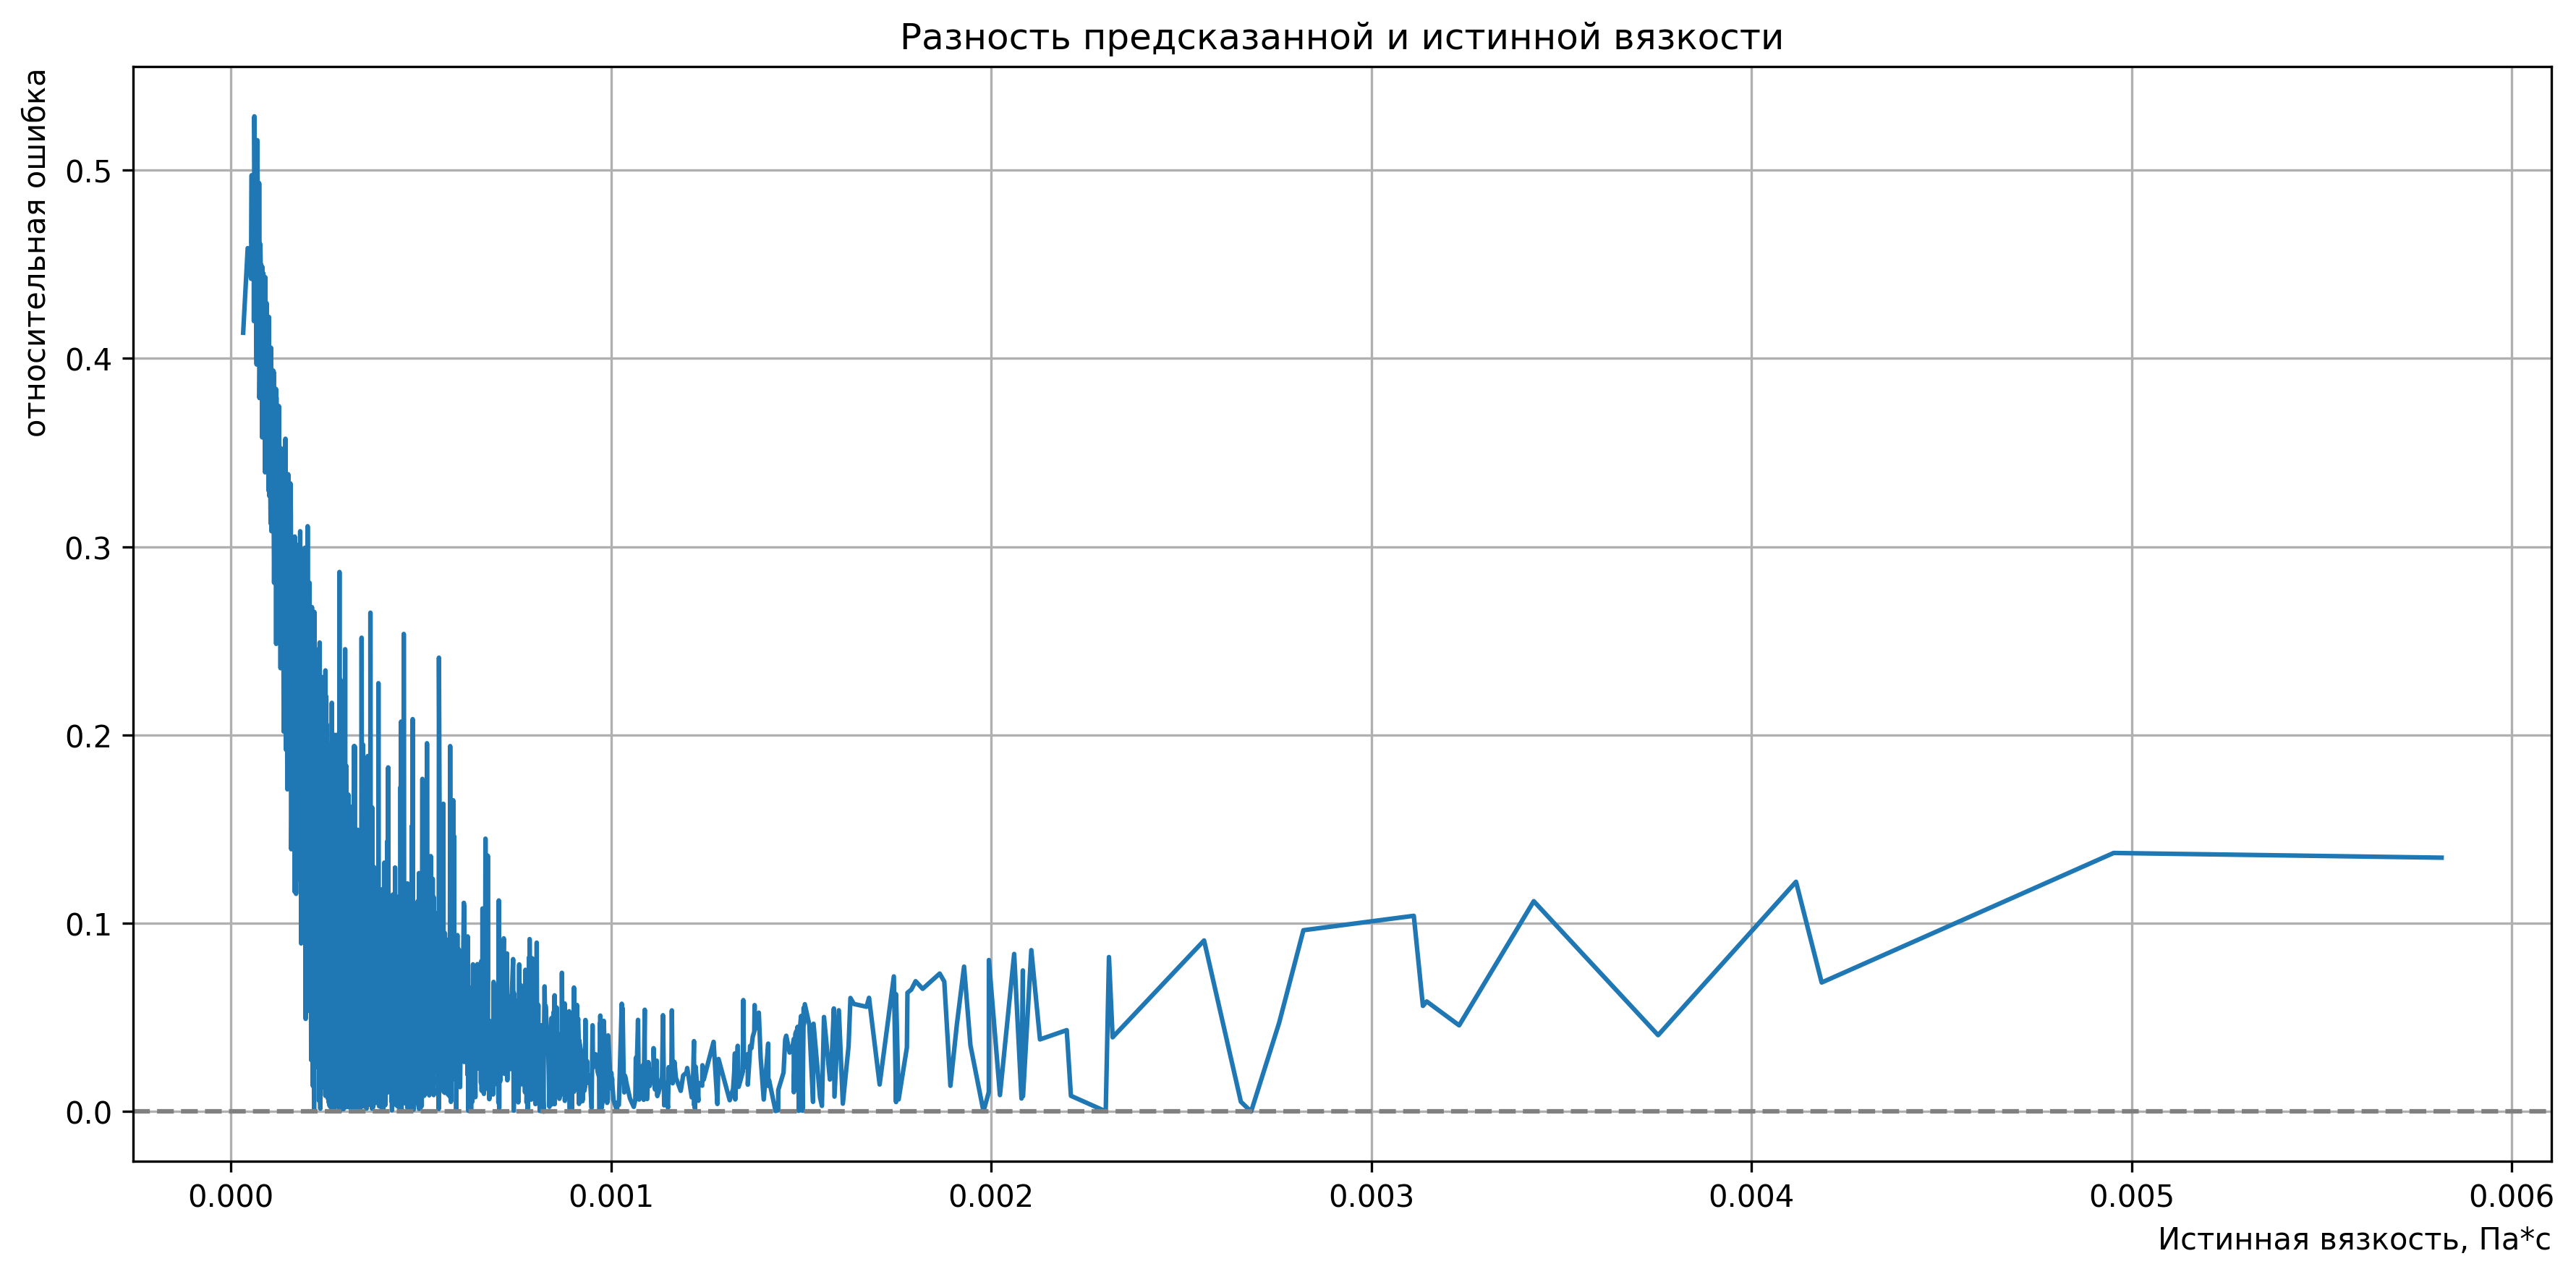
\includegraphics[width=0.8\textwidth]{MYS_percent.png}
        \caption{Зависимость относительной ошибки от истинного значения вязкости для модели MYS}
        \label{fig:mys_rmse}
    \end{figure}
    
    \begin{figure}[ht!]
        \centering
        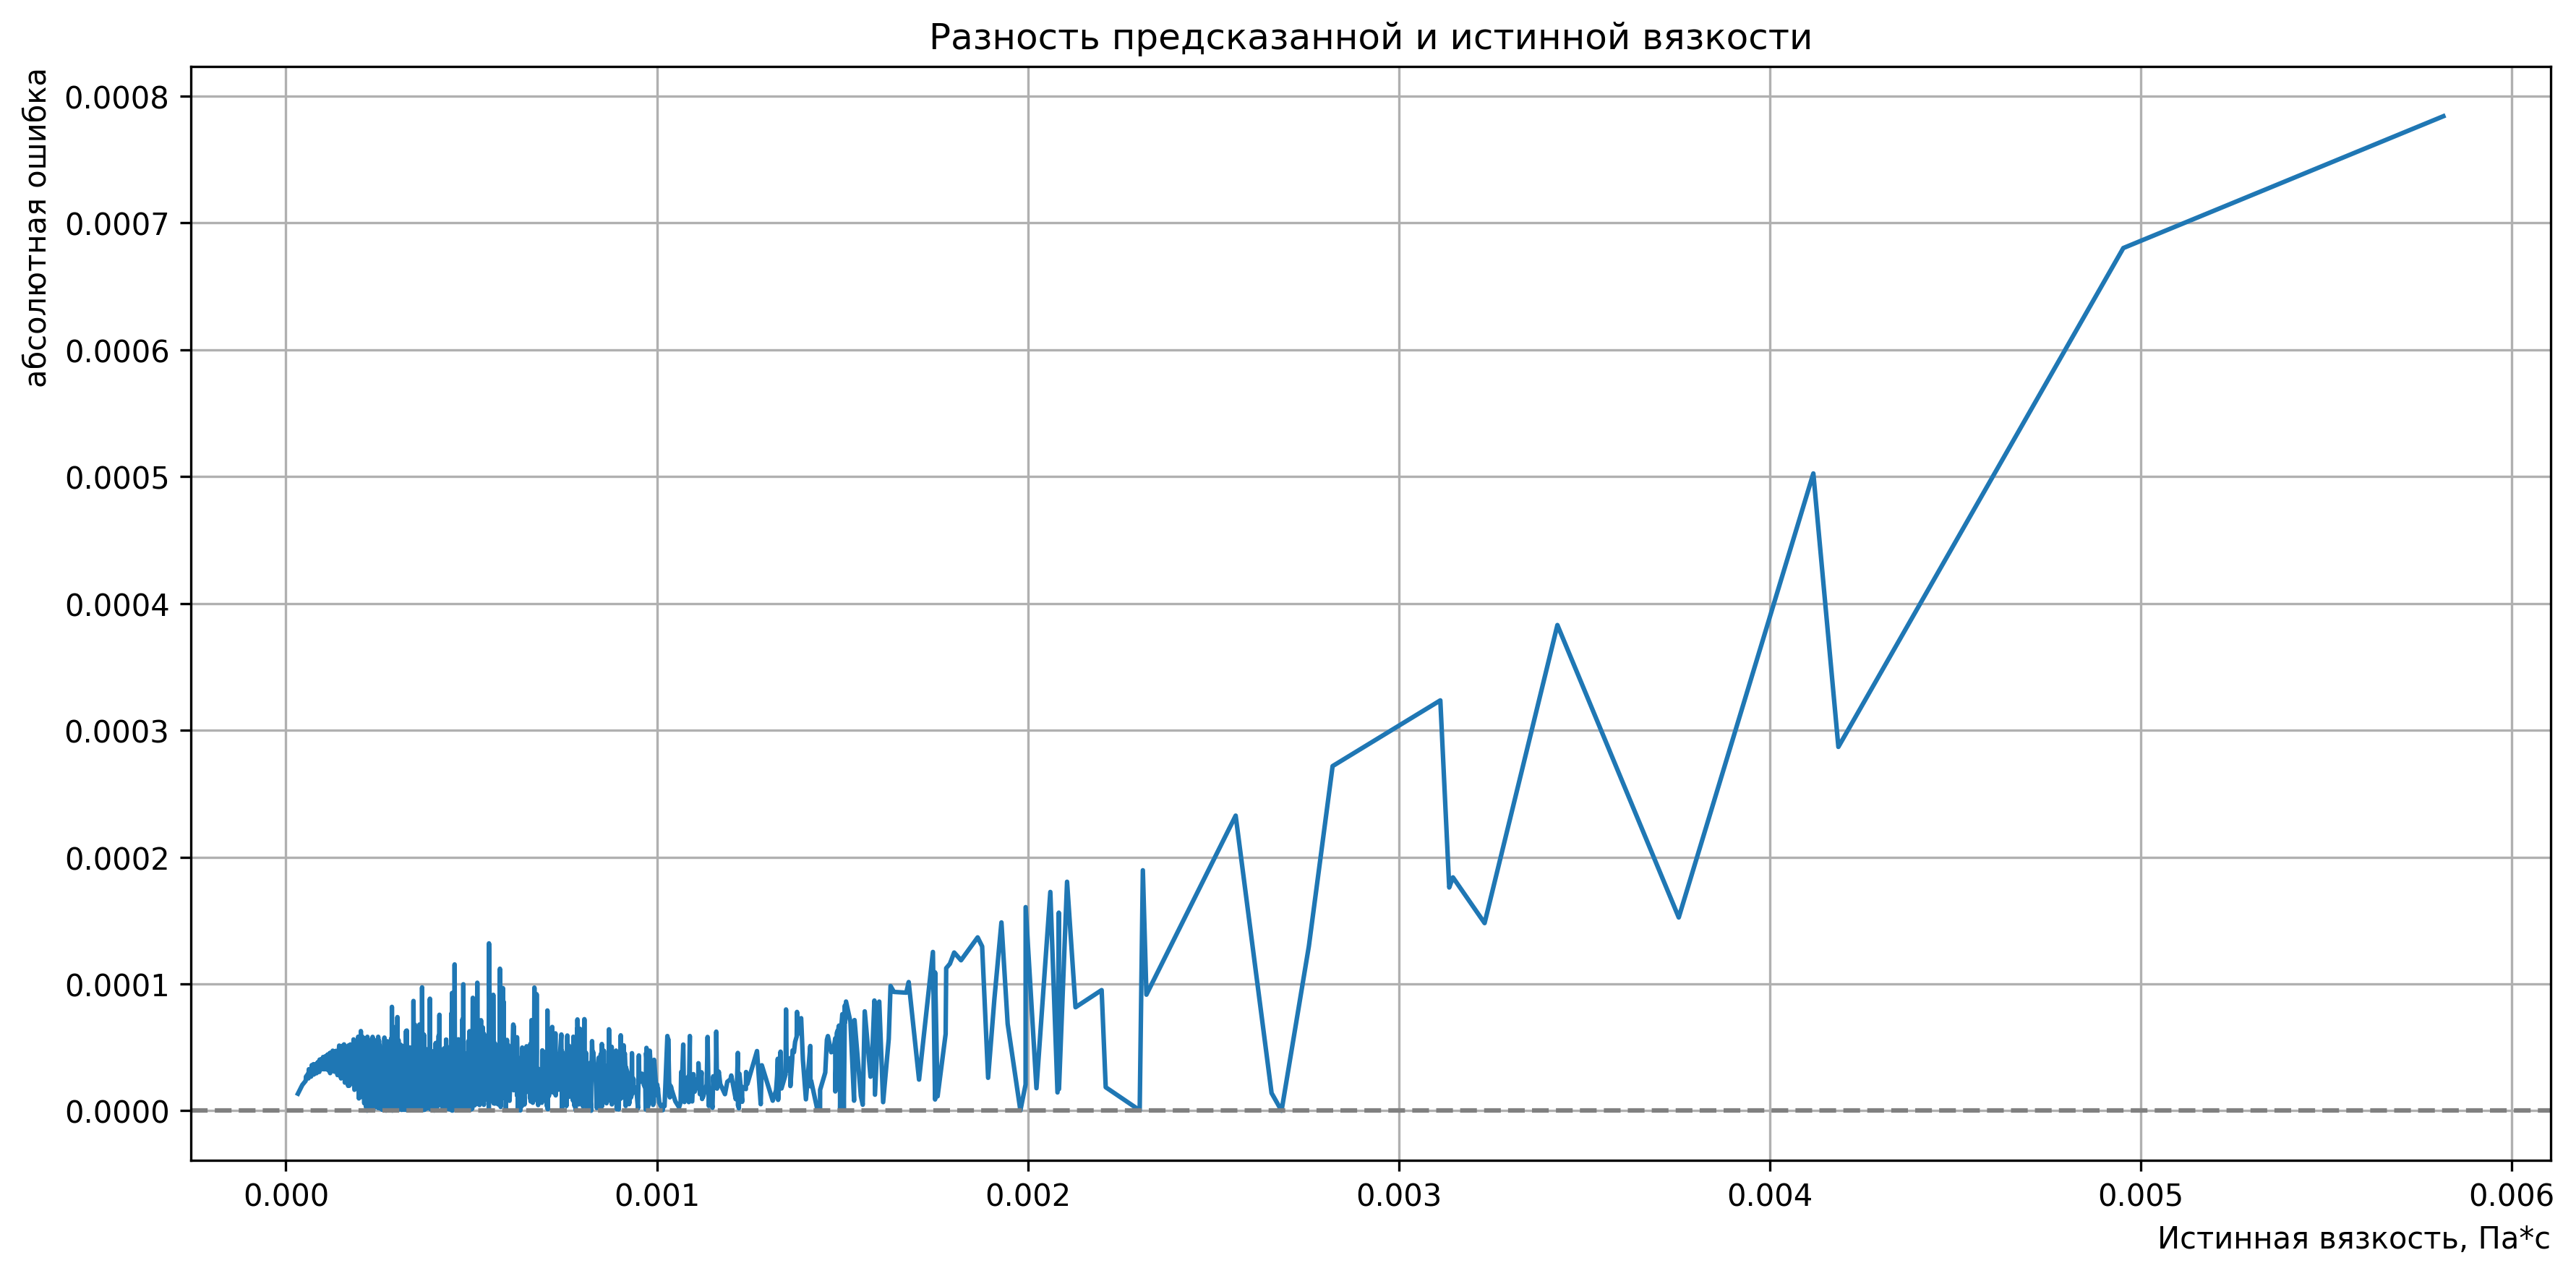
\includegraphics[width=0.8\textwidth]{MYS_rmse.png}
        \caption{Зависимость абсолютной ошибки от истинного значения вязкости для модели MYS}
        \label{fig:mys_relative_error}
    \end{figure}
    
    Для обобщения результатов были рассчитаны средние и медианные значения ошибок по каждому веществу. Данные представлены в таблице~\ref{tab:mys_stats}.
    \begin{table}[ht!]
      \TableNumberRight
      \begin{center}
        \textbf{Средние и медианные значения относительной и абсолютной ошибки модели MYS}
        \vspace*{\fill}
      \end{center}
      
      \vspace{0.8ex}
      \noindent
 
      \label{tab:mys_stats}
      \begin{tabular}{
        |l
        |S[table-format=1.3]
        |S[table-format=1.3]
        |S[table-format=1.2e-2]
        |S[table-format=1.2e-2]
        |}
        \hline
        \textbf{Вещество} & \textbf{Отн. ошибка, ср.} & \textbf{Отн. ошибка, мед.} & \textbf{Абс. ошибка, ср.} & \textbf{Абс. ошибка, мед.} \\
        \hline
        бутан     & 3.796 & 0.482 & 3.63e-05 & 2.45e-05 \\
        пентан    & 0.098 & 0.077 & 1.93e-05 & 1.98e-05 \\
        гексан    & 0.048 & 0.043 & 1.40e-05 & 1.22e-05 \\
        гептан    & 0.069 & 0.055 & 2.63e-05 & 2.25e-05 \\
        октан     & 0.086 & 0.069 & 3.05e-05 & 2.94e-05 \\
        нонан     & 0.040 & 0.044 & 2.65e-05 & 2.80e-05 \\
        декан     & 0.069 & 0.031 & 2.57e-05 & 2.26e-05 \\
        додекан   & 0.106 & 0.032 & 4.25e-05 & 3.04e-05 \\
        \hline
      \end{tabular}
    \end{table}
    
    Собранные данные позволяют наглядно оценить, в каких условиях модель MYS работает особенно хорошо или наоборот — начинает терять точность, что важно при дальнейшем сравнении с моделями машинного обучения. Можно сделать предположение, что ошибка моделей может оказаться выше на данных для бутана, додекана, октана и пентана по сравнению с остальными данными, так как для этих данных значения ошибок наиболее велики.

    Для данных без бутана значения основных трех метрик для модели MYS следующие:
    \begin{itemize}
      \item \textbf{RMSE}: \(4.85 \times 10^{-5} \) Па·с
      \item \textbf{Cредняя относительная ошибка}: \(7.88*10^-2\)
      \item \textbf{Средняя абсолютная ошибка}: \(2.99 \times 10^{-5} \) Па·с
    \end{itemize}

    Дополнительно можно оценить, насколько важным было вычисление коэффициента вязкости идеального газа. Если его занулить, то метрики модели становятся следующими:
    \begin{itemize}
      \item \textbf{RMSE}: \(5.03 \times 10^{-5} \) Па·с
      \item \textbf{Cредняя относительная ошибка}: \(9.11*10^-2\)
      \item \textbf{Средняя абсолютная ошибка}: \(3.14 \times 10^{-5} \) Па·с
    \end{itemize}

    Все метрики стали хуже, что и ожидалось. Особенно сильно увеличилась относительная ошибка. Это подтверждает то, что вязкость идеального газа дает наибольший вклад в случаях, когда итоговое значение вязкости мало.

  \subsection{Символьная регрессия}

    В качестве дополнительного подхода была протестирована символьная регрессия на базе библиотеки \texttt{PySR}. Метод направлен на построение компактных аналитических выражений, аппроксимирующих целевую функцию, строя математические выражения на основе признаков. В результате был получен аналитический вид зависимости вязкости от нескольких параметров вещества:

    Символьная регрессия была выполнена с использованием библиотеки \texttt{PySR}, основанной на генетическом поиске выражений с минимальной сложностью и максимальной точностью. В качестве признаков использовались параметры уравнения состояния CP-PC-SAFT, а в качестве целевой переменной — вязкость в Паскалях·секундах.

Для запуска модели использовались следующие параметры:

\begin{itemize}
  \item число итераций: \texttt{niterations = 1000};
  \item бинарные операторы: \( \{+, -, \times, \div \} \);
  \item унарные операторы: \( \{\exp, \log\} \);
  \item функция потерь: \( (x - y)^2 \);
  \item максимальная сложность выражения: \texttt{maxsize = 40};
  \item максимальная глубина дерева выражения: \texttt{maxdepth = 5};
  \item штраф за сложность (парсимония): \( \lambda = 0.001 \);
  \item оценка сложности операторов: \texttt{exp} и \texttt{log} — 3, остальные — 1.
\end{itemize}

Обучение модели проводилось на процессоре \texttt{11th Gen Intel\textsuperscript{\textregistered} Core\textsuperscript{TM} i7-1165G7} с использованием 8 потоков на 4 физических ядрах. Общая продолжительность вычислений составила около 30 минут. По завершении поиска модель автоматически выбрала наилучшее выражение по балансу между точностью и сложностью, которое приведено далее:
    
    \begin{equation}
    \hat{\eta} = \left( \frac{(v - 0.0003949) \cdot \sigma}{\dfrac{\epsilon / k_B}{s^{\text{res}}} + 1.7387} \right) - 0.0001168,
    \end{equation}
    
    где:
    \begin{itemize}
      \item \( \hat{\eta} \) — предсказанное значение вязкости [Па·с];
      \item \( v \) — мольный объём [м\(^3\)/моль];
      \item \( \sigma \) — диаметр сегмента для уравнения CP-PC-SAFT [\si{\angstrom}];
      \item \( \epsilon/k_B \) -- средняя энергия взаимодействия для уравнения CP-PC-SAFT [К];
      \item \( s^{\text{res}} \) — избыточная энтропия [Дж/(моль·К)].
    \end{itemize}

    Полученное выражение является достаточно компактным и легко интерпретируемым с точки зрения размерностей и физического смысла. Оно отражает функциональную зависимость вязкости от четырёх ключевых параметров: мольного объёма, размера сегмента, избыточной энтропии и глубины потенциальной ямы. При этом сложно дать однозначное объяснение данной формуле, что указывает на потенциальное наличие перекрёстных эффектов между ними. Например, числитель увеличивается с ростом мольного объёма и диаметра сегмента, что может быть связано с ростом внутреннего трения. Знаменатель, содержащий отношение энергии взаимодействия к энтропии, отражает сложную связь между термодинамической упорядоченностью и глубиной межмолекулярных взаимодействий. В целом, модель подчёркивает, что вязкость определяется не отдельным параметром, а их соотношением в конкретных условиях.

    \medskip
    
    На \autoref{fig:sr_rmse} и \autoref{fig:sr_percent} представлены графики абсолютной и относительной ошибки модели на основе символьной регрессии:
    
    \begin{figure}[ht!]
      \centering
      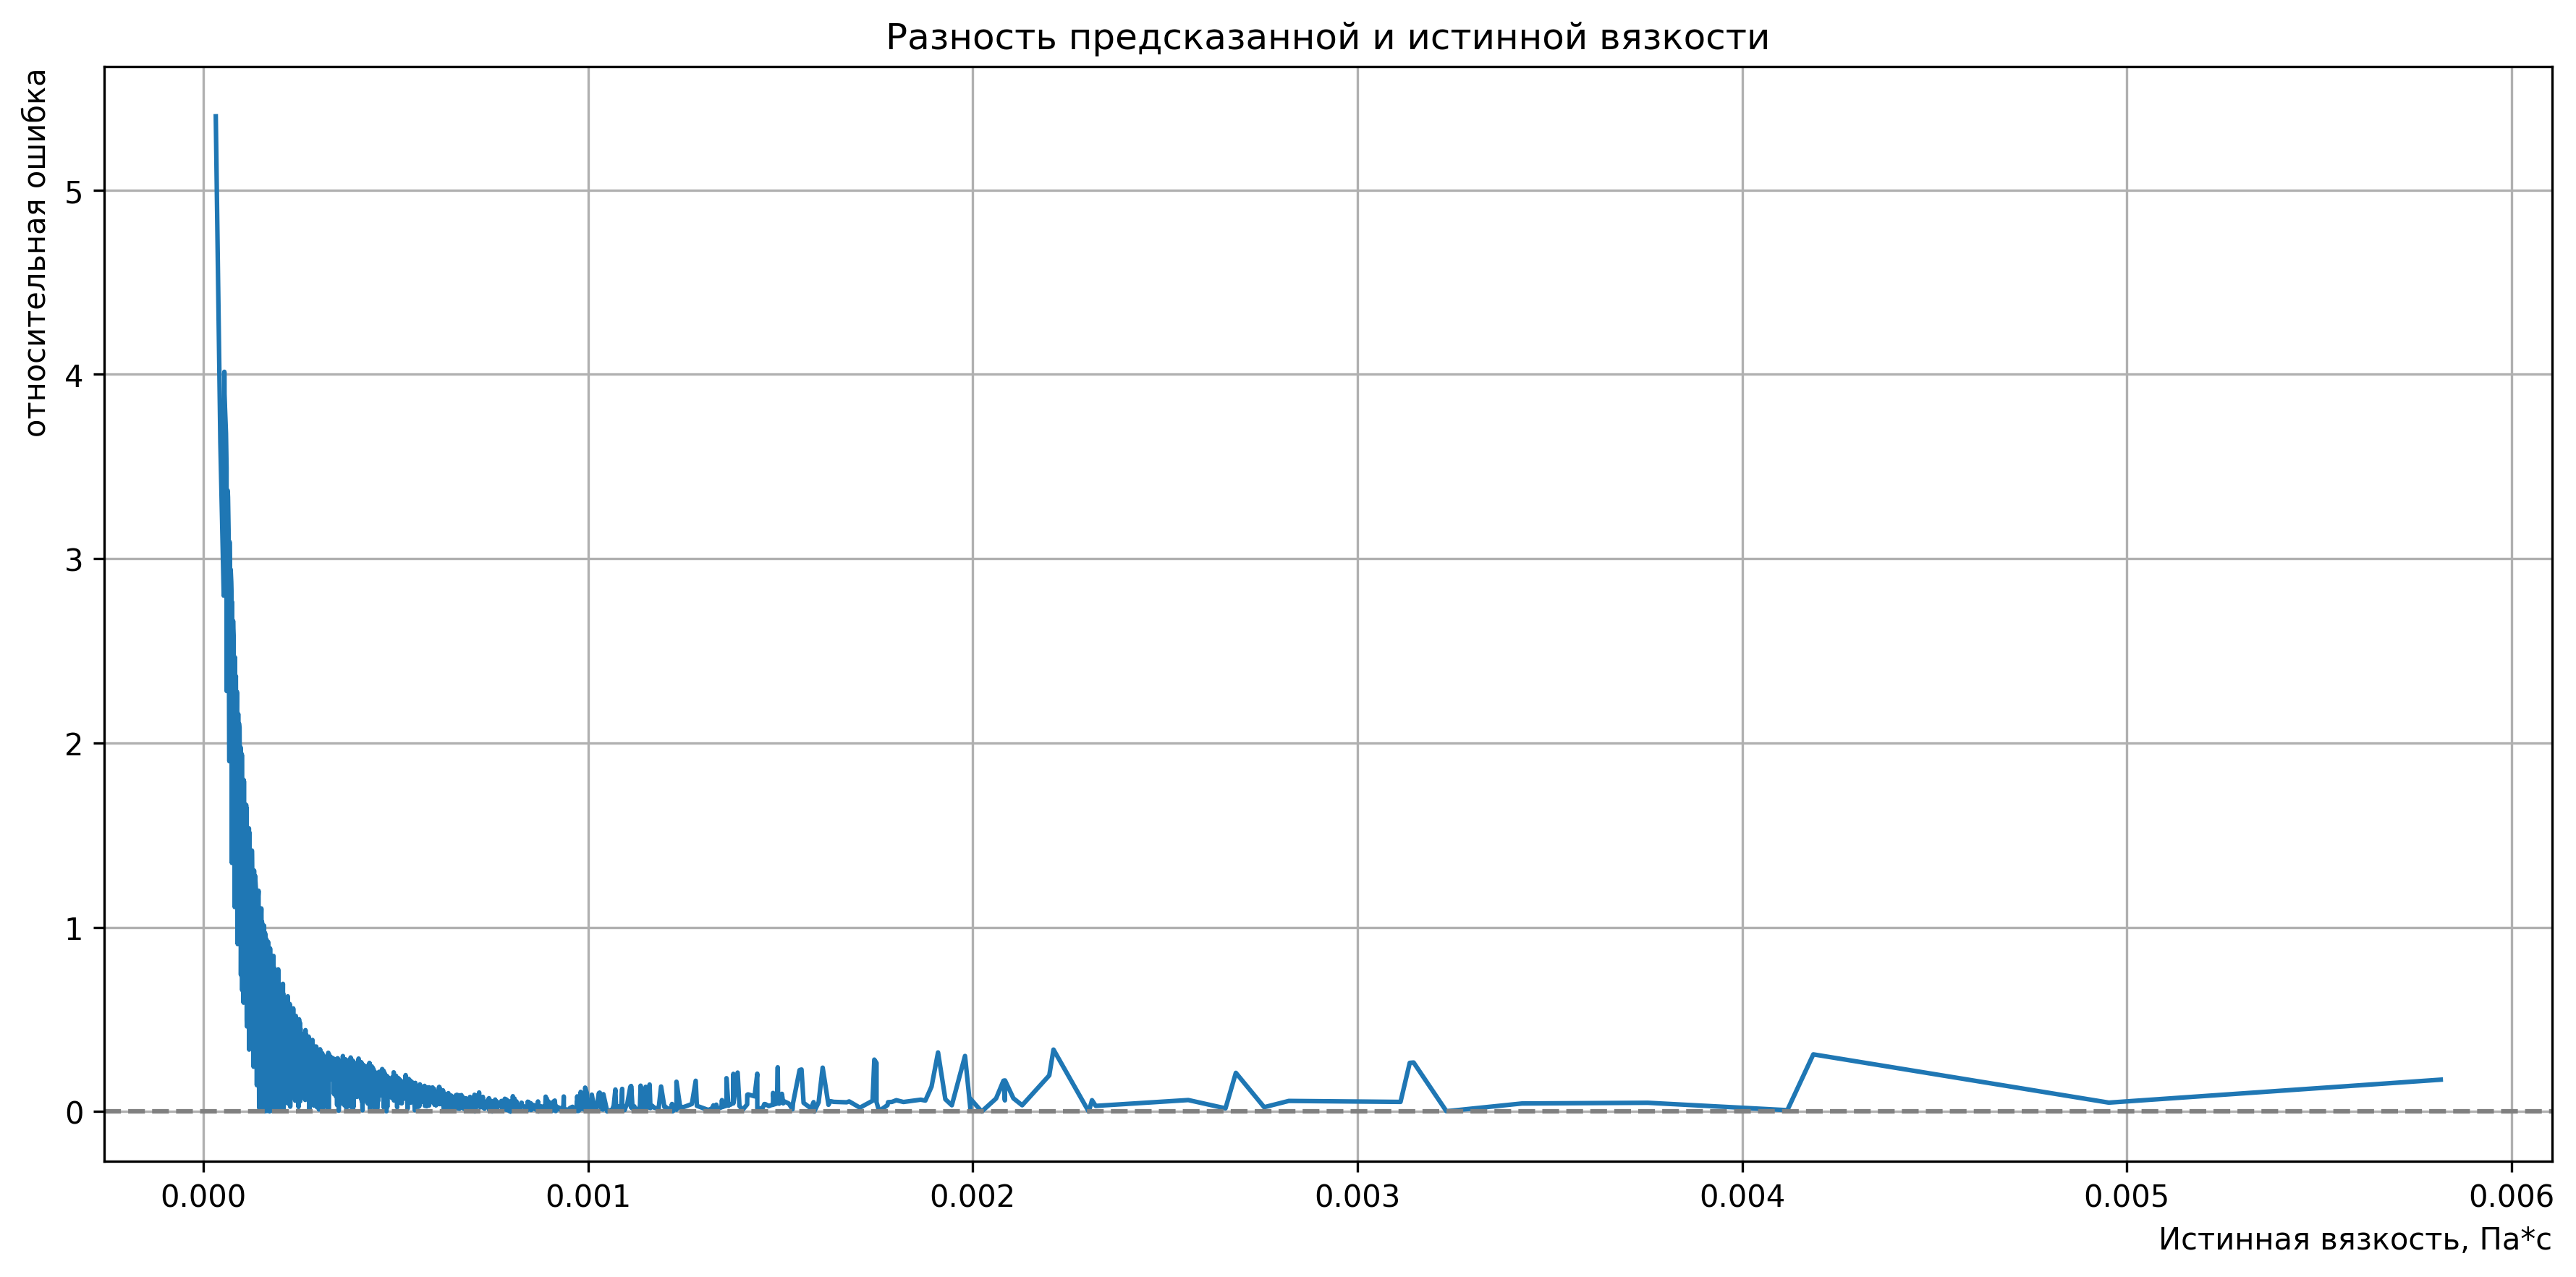
\includegraphics[width=0.8\textwidth]{SR_percent.png}
      \caption{Относительная ошибка символьной модели в зависимости от истинной вязкости}
      \label{fig:sr_percent}
    \end{figure}
    
    \begin{figure}[ht!]
      \centering
      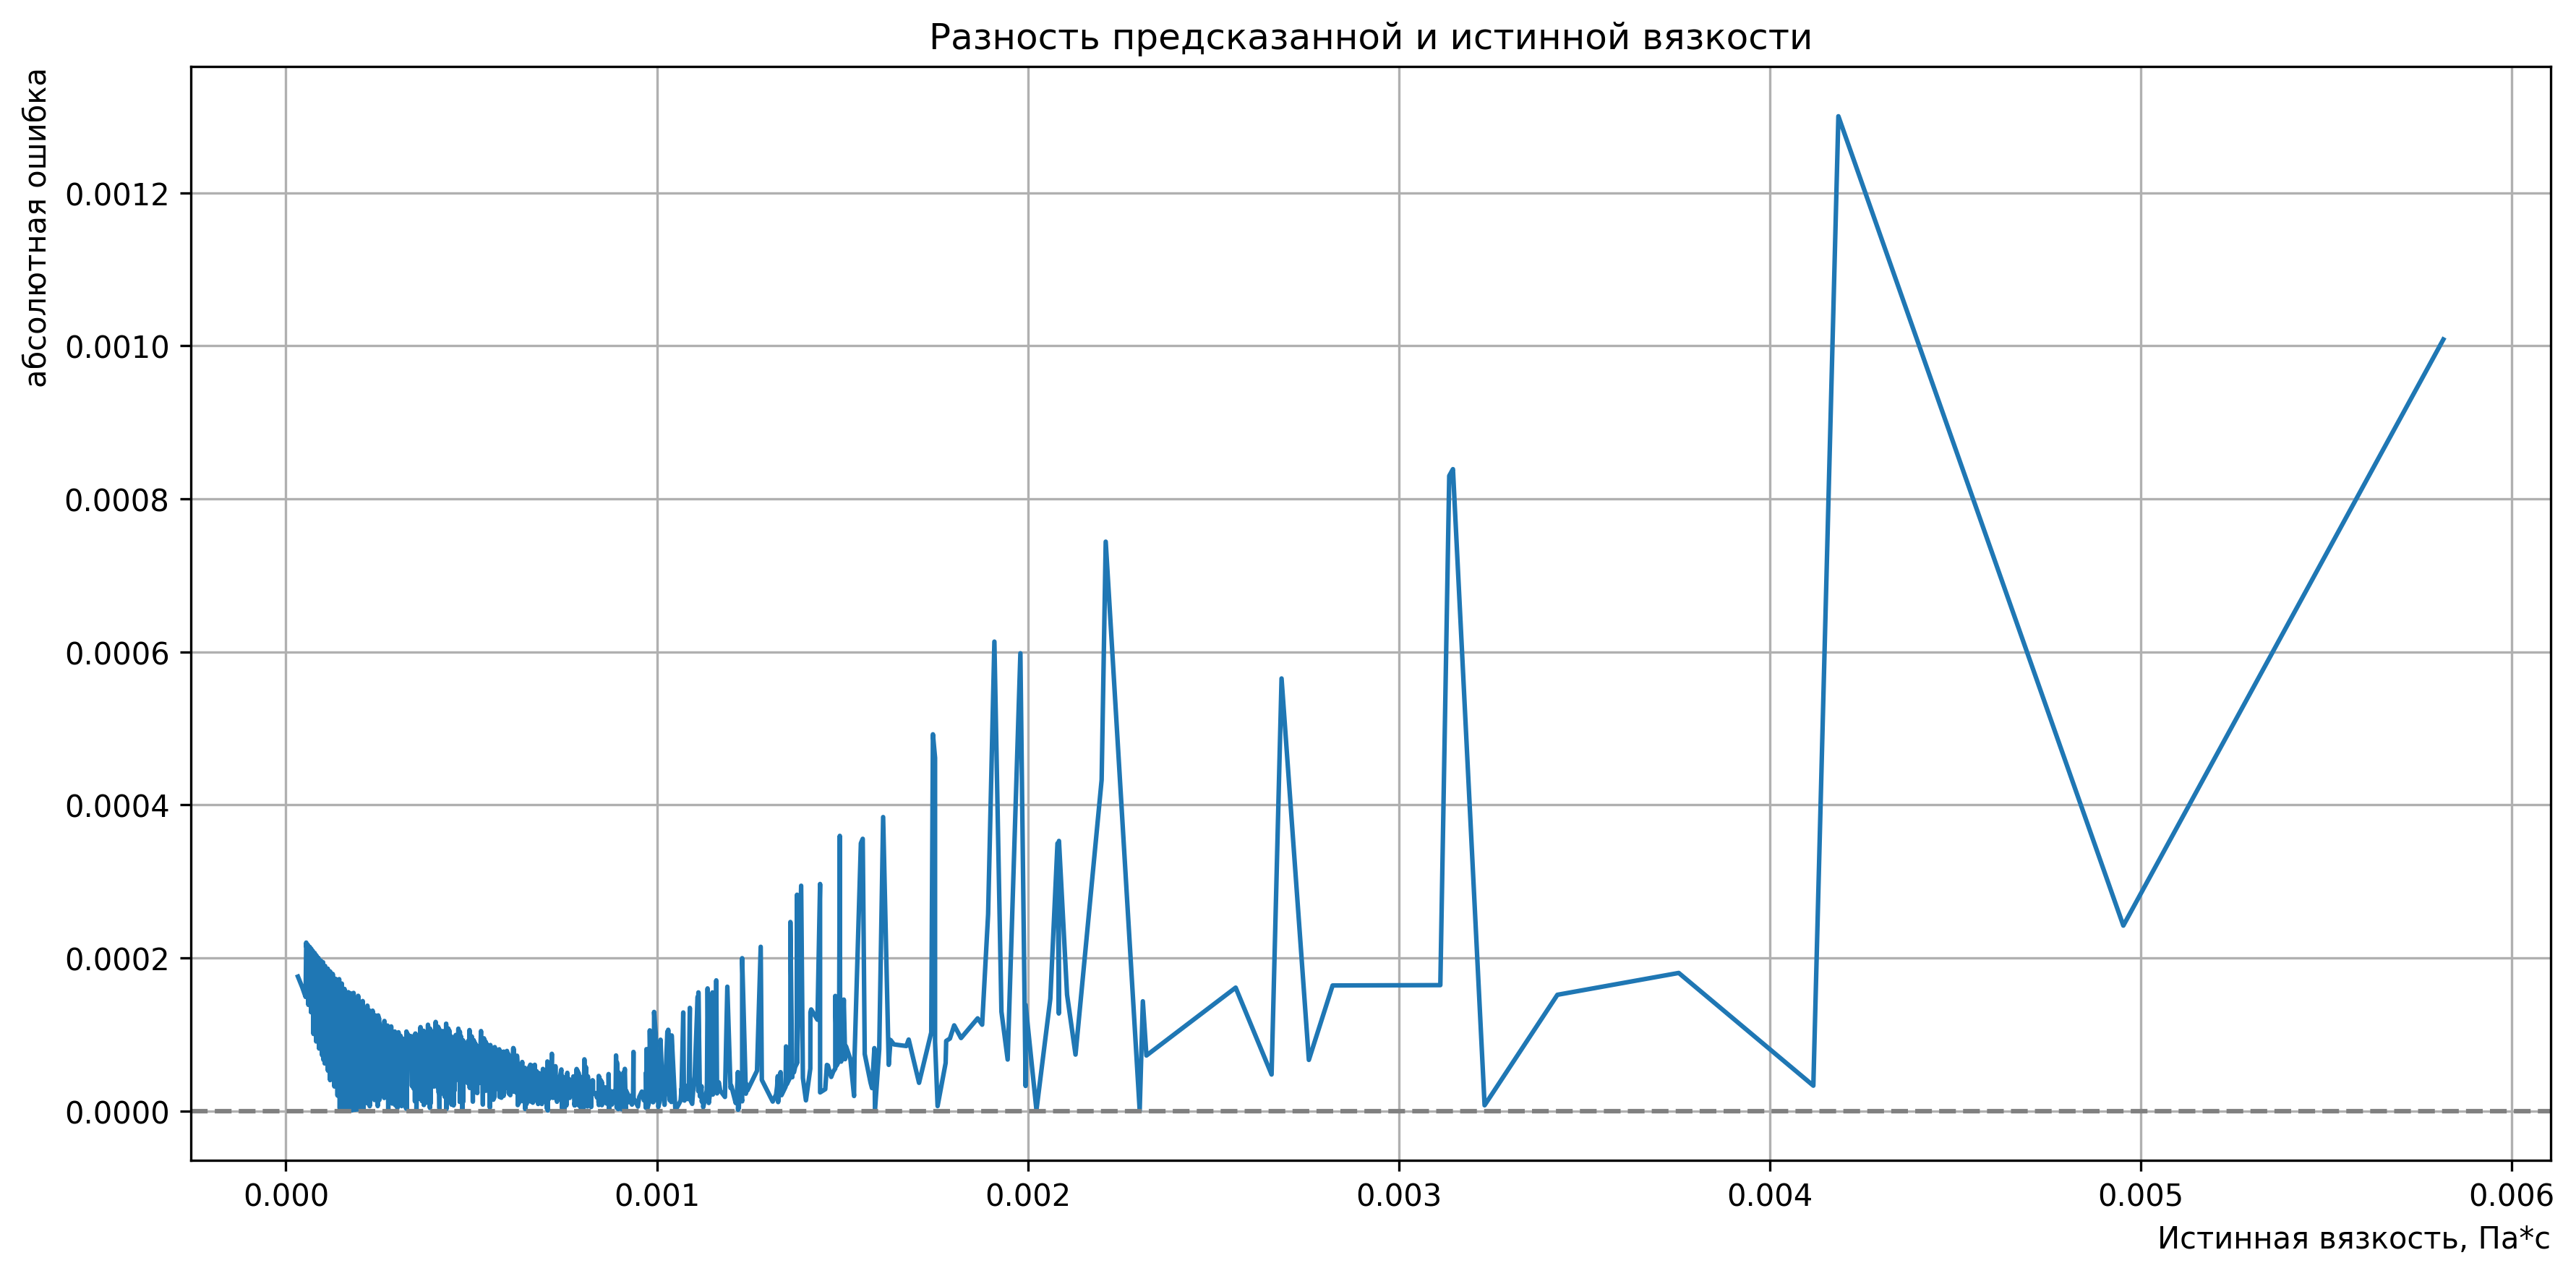
\includegraphics[width=0.8\textwidth]{SR_rmse.png}
      \caption{Абсолютная ошибка предсказания символьной модели}
      \label{fig:sr_rmse}
    \end{figure}
    
    \medskip
    
    Несмотря на простоту выражения, модель показала относительно приемлемую точность:
    
    \begin{itemize}
      \item RMSE: \( 9.87 \times 10^{-5} \) Па·с;
      \item Средняя абсолютная ошибка (MAE): \( 6.67 \times 10^{-5} \) Па·с;
      \item Средняя относительная ошибка (MRE): \( 0.231 \).
    \end{itemize}

    Также стоит отметить, что символьная регрессия тренировалась на полном наборе данных без разбиения на тестовую и тренировочную выборку. Вряд ли это сильно уменьшило значения ошибок ввиду сильной устойчивости к переобучению у данной модели, но результат мог бы быть потенциально хуже.
    
    Таким образом, символьная регрессия может быть полезным инструментом для построения простых аналитических аппроксимаций, особенно в условиях ограниченного количества данных или требований к интерпретируемости. Метод оказался полезным как дополнительный инструмент анализа, но не подошел в качестве основной модели. Отдельный интерс представляет оптимизация параметров запуска модели символьной регрессии или запуск алгоритма на более долгое время, так как генетические алгоритмы могут внезапно находить целые классы решений и улучшать свою точность на протяжении долгого времени без угрозы переобучения. 

 \subsection{Алгоритм автоматической генерации признаков}
 
    Начальные эксперименты с обучением простых моделей показали, что использование только исходных признаков приводит к значительно более низкой точности по сравнению с расширенным набором, включающим попарные произведения признаков. Краткий анализ продемонстрировал, что наибольший вклад в прирост точности дают лишь немногие из добавленных признаков. Это наблюдение мотивировало разработку алгоритма автоматической генерации признаков, направленного на отбор и итеративное улучшение наиболее информативных преобразований признаков.
  
    Алгоритм генерации новых признаков реализован в виде последовательности этапов:

    \begin{enumerate}
      \item \textbf{Генерация новых признаков с использованием элементарных операторов.}
      Унарные операторы (например, экспонента, логарифм, квадратный корень) применяются к каждому признаку индивидуально. Бинарные операторы ($+$, $-$, $*$, $/$) применяются ко всем возможным парам признаков.
      
      \item \textbf{Удаление некорректных или численно нестабильных признаков.}
      Исключаются признаки, нарушающие элементарные арифметические правила, например, ведущие к делению на ноль или взятию логарифма от отрицательных чисел. Также отбрасываются признаки с чрезмерно большими значениями, способные вызвать переполнение при хранении в формате \texttt{float32}.
      
      \item \textbf{Удаление избыточных признаков.}
      Исключаются признаки, обладающие высокой взаимной корреляцией или практически идентичные. В частности:
      \begin{itemize}
      \item Если векторная норма разности нормализованных признаков меньше порогового значения (например, $10^{-8}$).
      \item Если коэффициент корреляции Пирсона между признаками превышает заданный уровень (например, 0.998).
      \end{itemize}
      В случае дублирования предпочтение отдается более короткому признаку (с меньшим числом операций в формуле).
      
      \item \textbf{Снижение общего числа признаков.}
      Если число новых признаков превышает установленный лимит (в нашем случае --- не более $1/5$ от общего количества объектов в данных), выбирается подмножество наиболее компактных признаков.
      Отбор осуществляется с использованием функции \texttt{random.choices} из стандартной библиотеки Python, где каждому признаку присваивается вес, пропорциональный $1/(1 + \texttt{len})^3$, где \texttt{len} --- количество операций, необходимых для вычисления признака.
      
      \item \textbf{Обучение моделей на расширенном наборе признаков.}
      Данные делятся на обучающую и тестовую выборки (примерно 80\% и 20\% соответственно) с использованием \texttt{sklearn.model\_selection.train\_test\_split}, при этом значение \texttt{seed} фиксируется для воспроизводимости результатов. Тестовая выборка не участвует в обучении и используется исключительно для оценки качества моделей.
      
      \item \textbf{Оценка важности признаков.}
      Для каждой модели вычисляется список признаков, отсортированных по убыванию значимости. Требуется, чтобы каждая модель поддерживала метод оценки важности признаков. Методы расчёта будут рассмотрены далее в описании моделей.
      
      \item \textbf{Добавление информативных признаков.}
      В итоговый набор добавляются признаки, попавшие в число 10 наиболее важных хотя бы для одной из моделей (если они ещё не были добавлены ранее). Выбор размера этого списка балансирует между скоростью скоростью заполнения признакового пространства и устойчивостью моделей к переизбыточности.
      
      \item \textbf{Удаление неинформативных признаков.}
      Из признакового пространства исключаются признаки, оказавшиеся в числе 20 наименее значимых одновременно для всех моделей. Это достигается через пересечение списков слабейших признаков, сформированных для каждой модели. Выбор размера списка влияет на баланс между уменьшением шума и сохранением разнообразия признаков.
      
      \item \textbf{Сохранение текущего состояния.}
      Через фиксированные интервалы итераций полный список активных признаков сохраняется в CSV-файл, что позволяет продолжать генерацию признаков в дальнейшем с текущего состояния.
      
      \item \textbf{Итеративное повторение.}
      Описанный алгоритм повторяется заданное число раз, после чего проводится итоговая оценка качества моделей.

      \item \textbf{Строгий отсев.}
      По окончании итеративного улучшения производится строгий отсев коэффициентов. На этом этапе промежуточные параметры, которые могут быть важны, как составные части сложных признаков становятся не важны, поэтому их можно отбросить. Осталяется примерно 50 коэффициентов, которые будут использованы для итоговой валидации методов.
    \end{enumerate}
    
    Следует отметить, что все численные параметры, использованные в процессе — включая количество добавляемых и удаляемых признаков, пороговые значения для корреляции и различия признаков, ограничения на общее количество признаков и веса в функции выбора — были подобраны эмпирически на основе анализа поведения моделей в ходе десятков независимых запусков. Эти значения показали хорошую эффективность в контексте текущего исследования, однако не претендуют на универсальность и не являются строгими рекомендациями. Их настройка должна осуществляться с учётом специфики конкретной задачи и свойств исходных данных.

  \subsection{Выводы по главе}

    В данной главе были рассмотрены интерпретируемые подходы к моделированию вязкости и представлен алгоритм генерации новых признаков. Анализ модели MYS показал, что, несмотря на физическую обоснованность, её точность ограничена, особенно на участках с низкой вязкостью, где вклад идеального газа становится критичен. Полученное с помощью символьной регрессии аналитическое выражение продемонстрировало разумный баланс между точностью и компактностью, подтверждая потенциал метода для первичного анализа данных.
    
    Разработанный алгоритм автоматической генерации признаков позволил обогатить исходный набор параметров новыми комбинациями, значимость которых оценивалась с точки зрения влияния на точность моделей. Итеративная природа алгоритма, а также строгий отбор и удаление признаков, должны позволить сохранить интерпретируемость и устойчивость моделей. Полученные признаки и формулы станут основой для дальнейшего обучения моделей и сравнения с MYS друг другом.

\section{Обучение и сравнение ML моделей}

  На этапе построения моделей машинного обучения рассматривались различные алгоритмы: линейная регрессия, решающие деревья, метод случайных соседей, случайный лес, а также нейросети. Однако от нейросетей было решено отказаться — они показали избыточную сложность в тренировке и интерпретации результатов, не обеспечивая при этом существенного выигрыша в точности.
  
  Для повышения качества обучения и анализа обобщающей способности моделей были проведены несколько экспериментов с разным составом данных. В частности, в большинстве экспериментов бутан был исключён из обучающей выборки. Это объясняется тем, что он представлен в базе в основном в газовой фазе, и на таких точках относительная ошибка теряет смысл: даже небольшое абсолютное отклонение приводит к очень высокой относительной погрешности. Хоть удаление бутана приводило к увеличению RMSE и MAE, но делало результаты более интерпретируемыми и устойчивыми.
  
  \begin{minipage}{\textwidth}
    \textbf{Признаки:}
    \begin{itemize}
      \item Базовый набор -- температура, давление, параметры CP-PC-SAFT;
      \item Расширенный набор -- признаки, сгенерированные автоматически и отобранные по важности.
    \end{itemize}
  \end{minipage}
  
  \begin{minipage}{\textwidth}
    \textbf{Модели:}
    \begin{itemize}
      \item Метод ближайших соседей;
      \item Линейная регрессия;
      \item Случайный лес.
      % \item Комбинирующая модель (ансамбль лучших моделей).
    \end{itemize}
  \end{minipage}
  
  \begin{minipage}{\textwidth}
    \textbf{Варианты разбиения данных:}
    \begin{itemize}
      \item Классическое случайное разбиение 80\% / 20\% — для оценки максимальной точности на тестовой выборке;
      \item Обратное разбиение 20\% / 80\% — для оценки устойчивости и обобщающей способности.
      % \item Разбиение по веществам — обучение на части соединений и тестирование на других, что позволяет оценить способность модели обобщать на новые вещества.
    \end{itemize}
  \end{minipage}
  
  \begin{minipage}{\textwidth}
    \textbf{Метрики качества:}
    \begin{itemize}
      \item RMSE (среднеквадратичная ошибка);
      \item MAE (средняя абсолютная ошибка);
      \item MRE (средняя относительная ошибка).
    \end{itemize}
  \end{minipage}

  Для получения наиболее достоверных значений метрик качества было использовано усреднение по множеству итераций. Как правило проводилось по 20 независимых обучений/тестов. Ошибки были подсчитаны на совместных предсказаниях со всех итераций.

  \subsection{Метод ближайших соседей}

    Метод \(k\) ближайших соседей (KNN) является одним из самых простых и интерпретируемых методов машинного обучения. Он не требует явной фазы обучения: предсказание для новой точки основывается на значениях целевой переменной у \(k\) ближайших по признаковому пространству соседей. В данной работе этот метод использовался как базовая отправная точка, позволяющая оценить нижнюю границу точности, которой можно достичь даже без сложной внутренней структуры модели. Предполагалось, что обобщающая способность KNN будет крайне ограниченной.

    Для реализации метода была использована реализация \texttt{KNeighborsRegressor} из \texttt{sklearn.neighbors} на языке Python. Параметр количества ближайших соседей был выбран равным 3. Такой параметр давал лучшее значение RMSE во всех тестах далее. Данные были отнормированы перед использованием этого метода.

    \subsubsection{Оценка точности на большом обучающем наборе}

      На первом этапе метод был протестирован на базовом наборе признаков (температура, давление и параметры CP-PC-SAFT) при обучении на 80\% данных. В этом случае модель показала хорошие значения средней относительной ошибки, однако RMSE оказался сравнительно высоким. Это указывает на наличие небольшого числа точек с особенно высокой ошибкой предсказания.
      
      \begin{figure}[ht!]
        \centering
        \begin{subfigure}{0.48\textwidth}
            \centering
            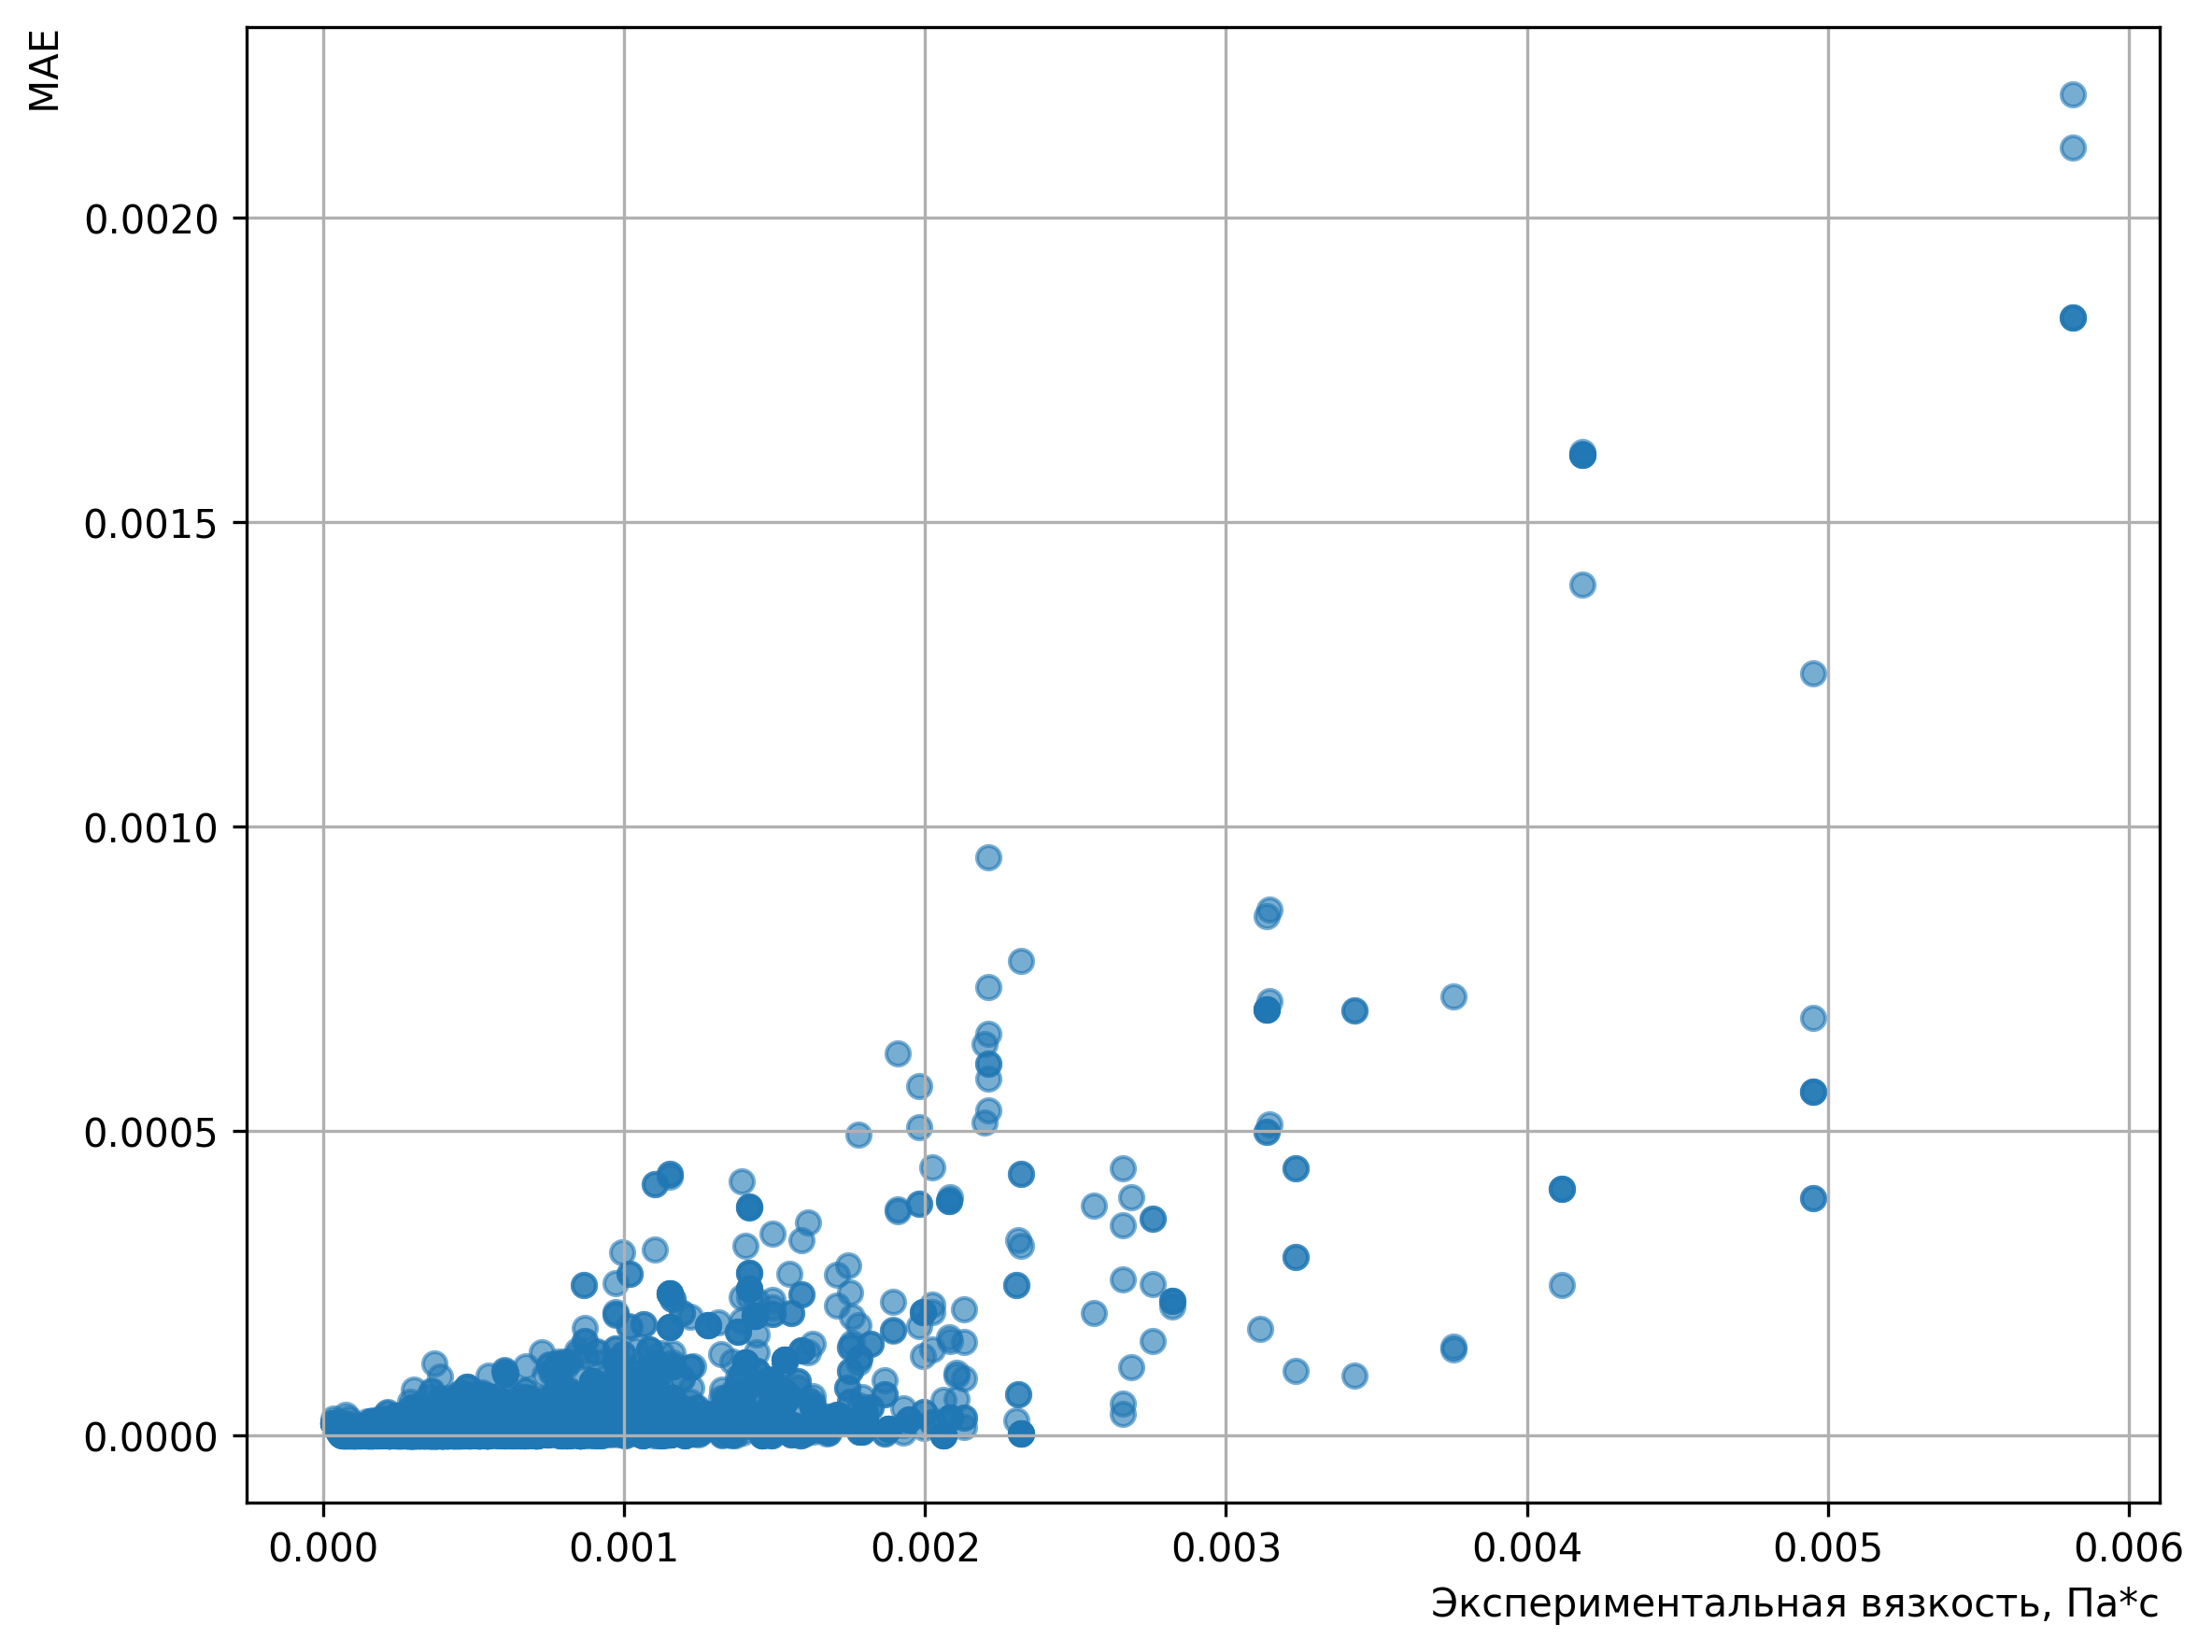
\includegraphics[width=\linewidth]{knn/MAE_KNN (k=3)_0.2_base.png}
            \caption{Абсолютная ошибка}
        \end{subfigure}
        \hfill
        \begin{subfigure}{0.48\textwidth}
            \centering
            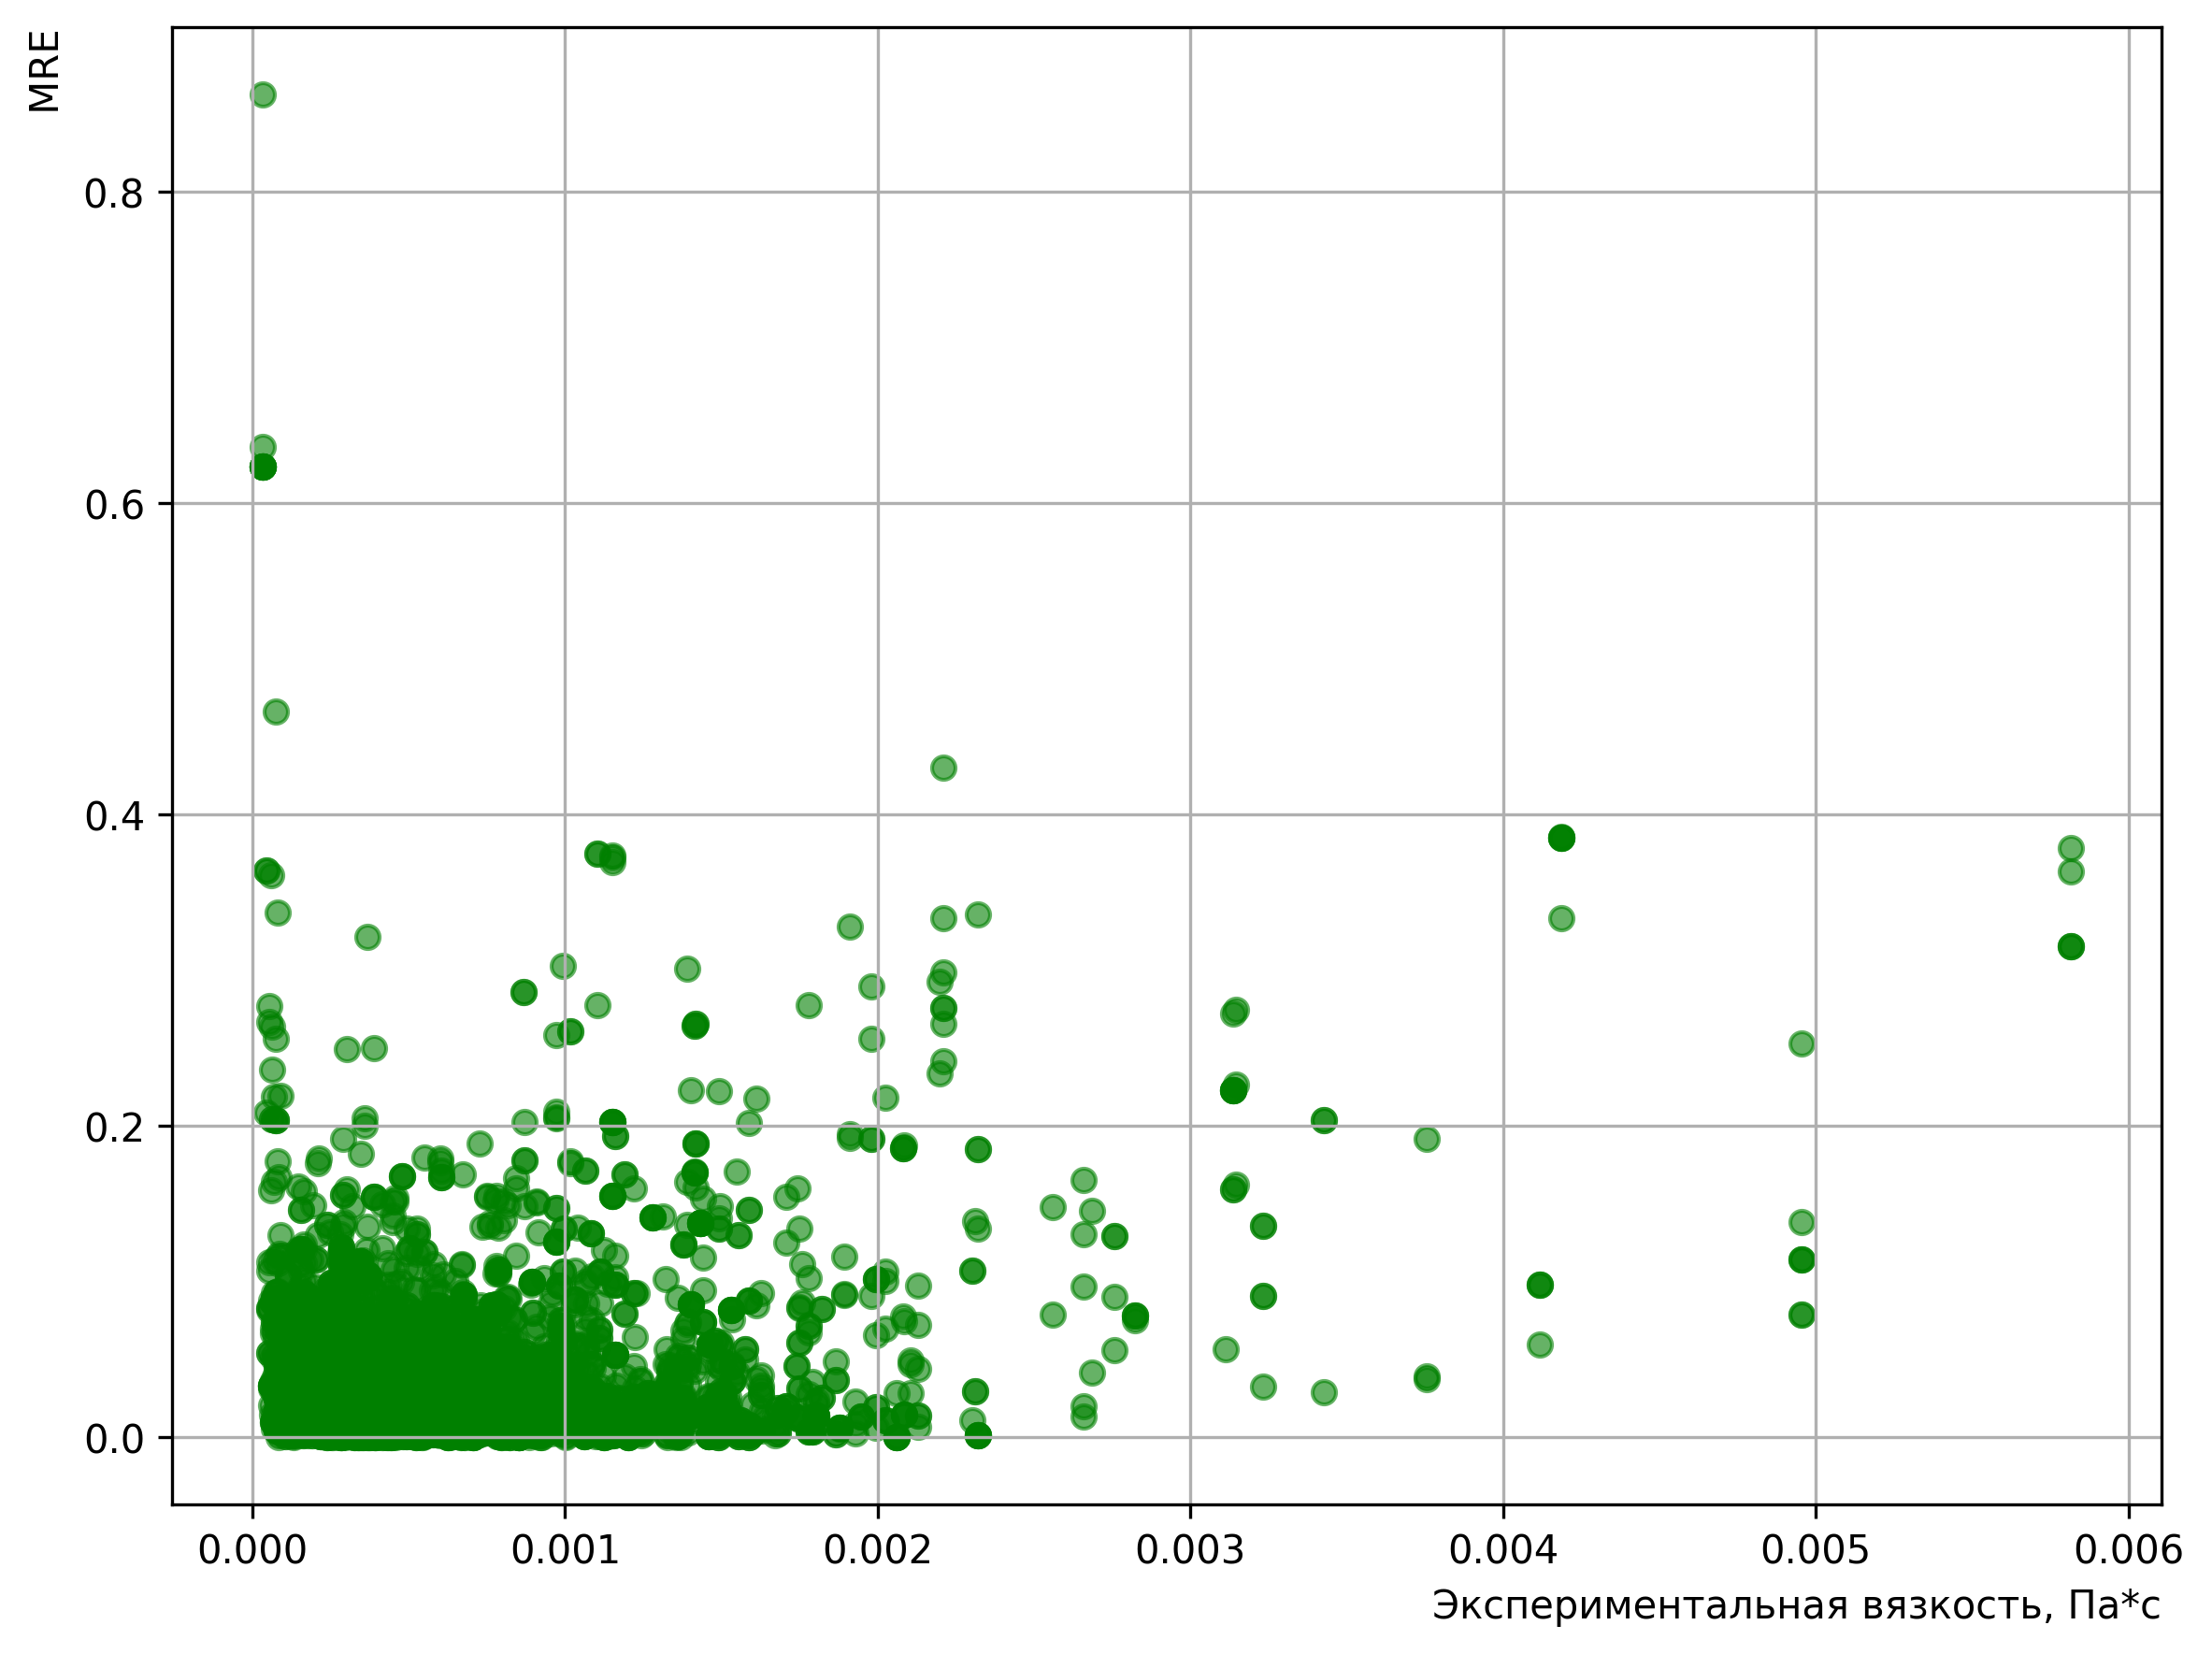
\includegraphics[width=\linewidth]{knn/MRE_KNN (k=3)_0.2_base.png}
            \caption{Относительная ошибка}
        \end{subfigure}
        \caption{Зависимость ошибки модели KNN от истинных значений вязкости. Базовый набор данных, большая обучающая выборка.}
        \label{fig:knn_errors_02_base}
      \end{figure}
      
      \begin{minipage}{\textwidth}
        \textbf{Метрики качества (базовые признаки, обучающая выборка 80\%):}
        \begin{itemize}
          \item RMSE: \( 9.09 \times 10^{-5} \) Па·с;
          \item MAE: \( 2.48 \times 10^{-5} \) Па·с;
          \item MRE: \( 0.0325 \).
        \end{itemize}
      \end{minipage}

    \subsubsection{Оценка на ограниченных данных}

      Чтобы оценить способность модели к обобщению, объёмы тренировочной и тестовой выборок были поменяны местами (20\% обучения, 80\% теста). Как и ожидалось, точность предсказаний существенно снизилась: модель стала хуже справляться с ранее не встречавшимися данными, уступая модели MYS по всем метрикам.
      
      \begin{figure}[ht!]
        \centering
        \begin{subfigure}{0.48\textwidth}
            \centering
            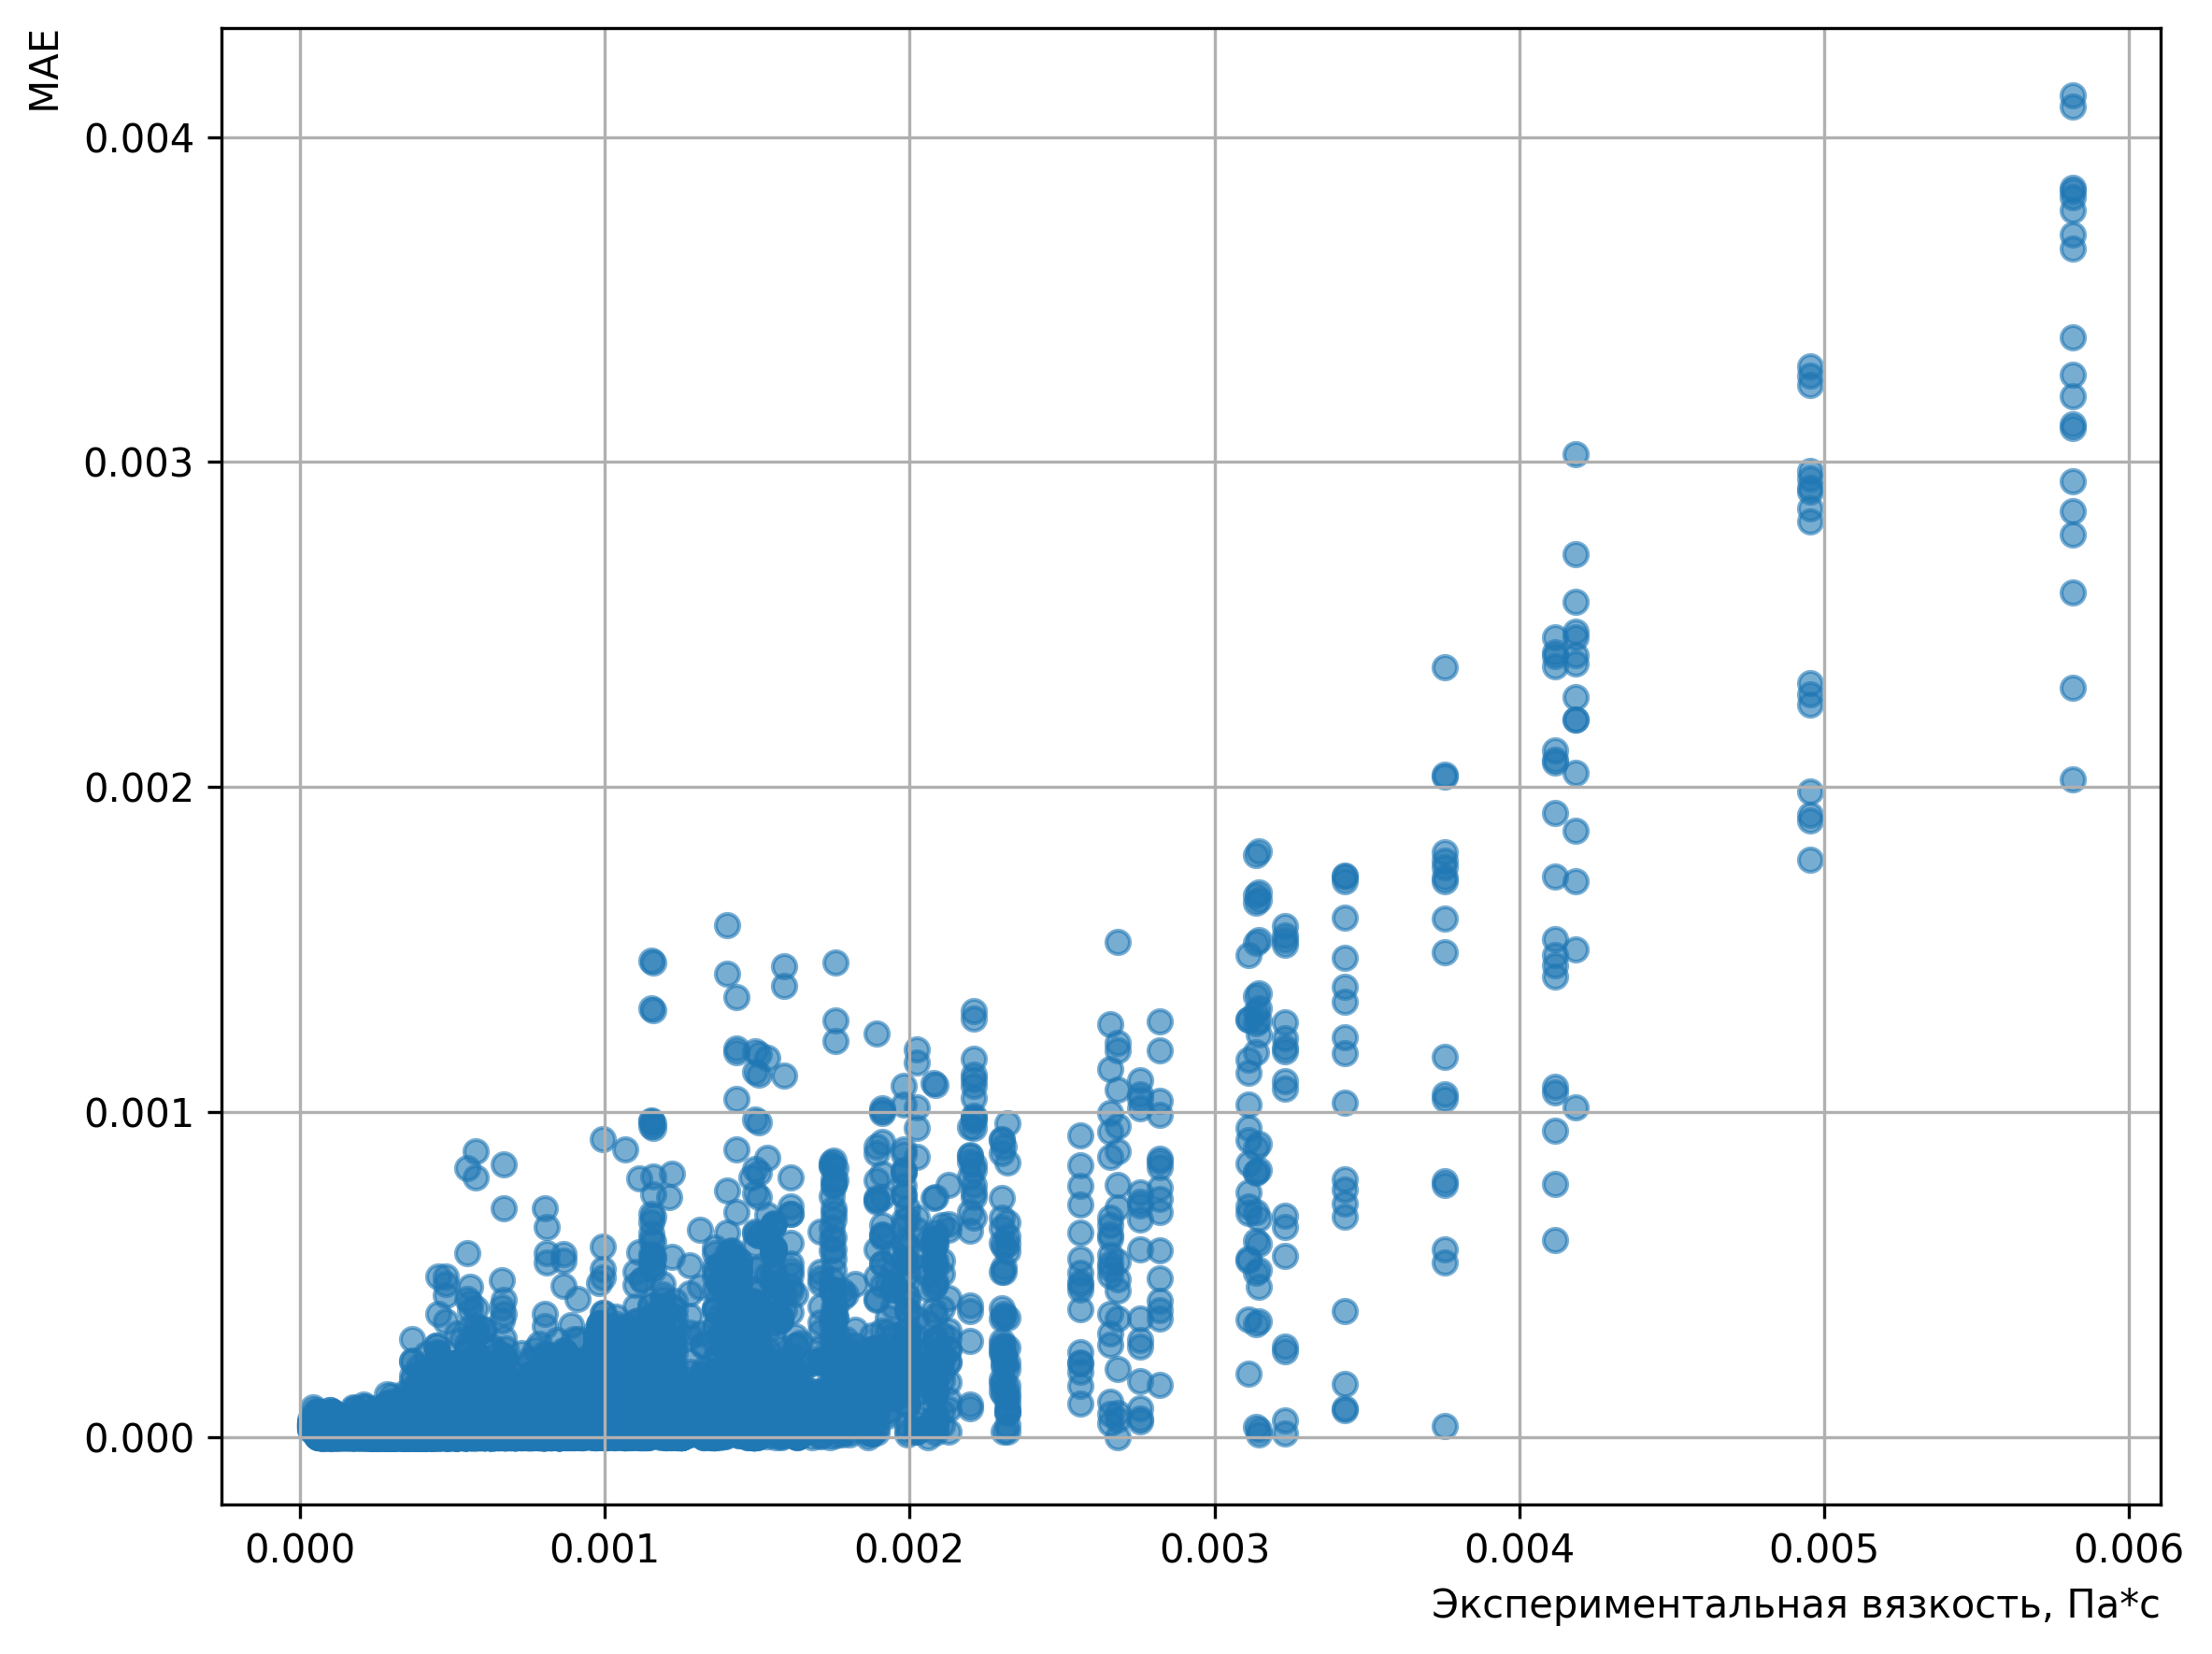
\includegraphics[width=\linewidth]{knn/MAE_KNN (k=3)_0.8_base.png}
            \caption{Абсолютная ошибка}
        \end{subfigure}
        \hfill
        \begin{subfigure}{0.48\textwidth}
            \centering
            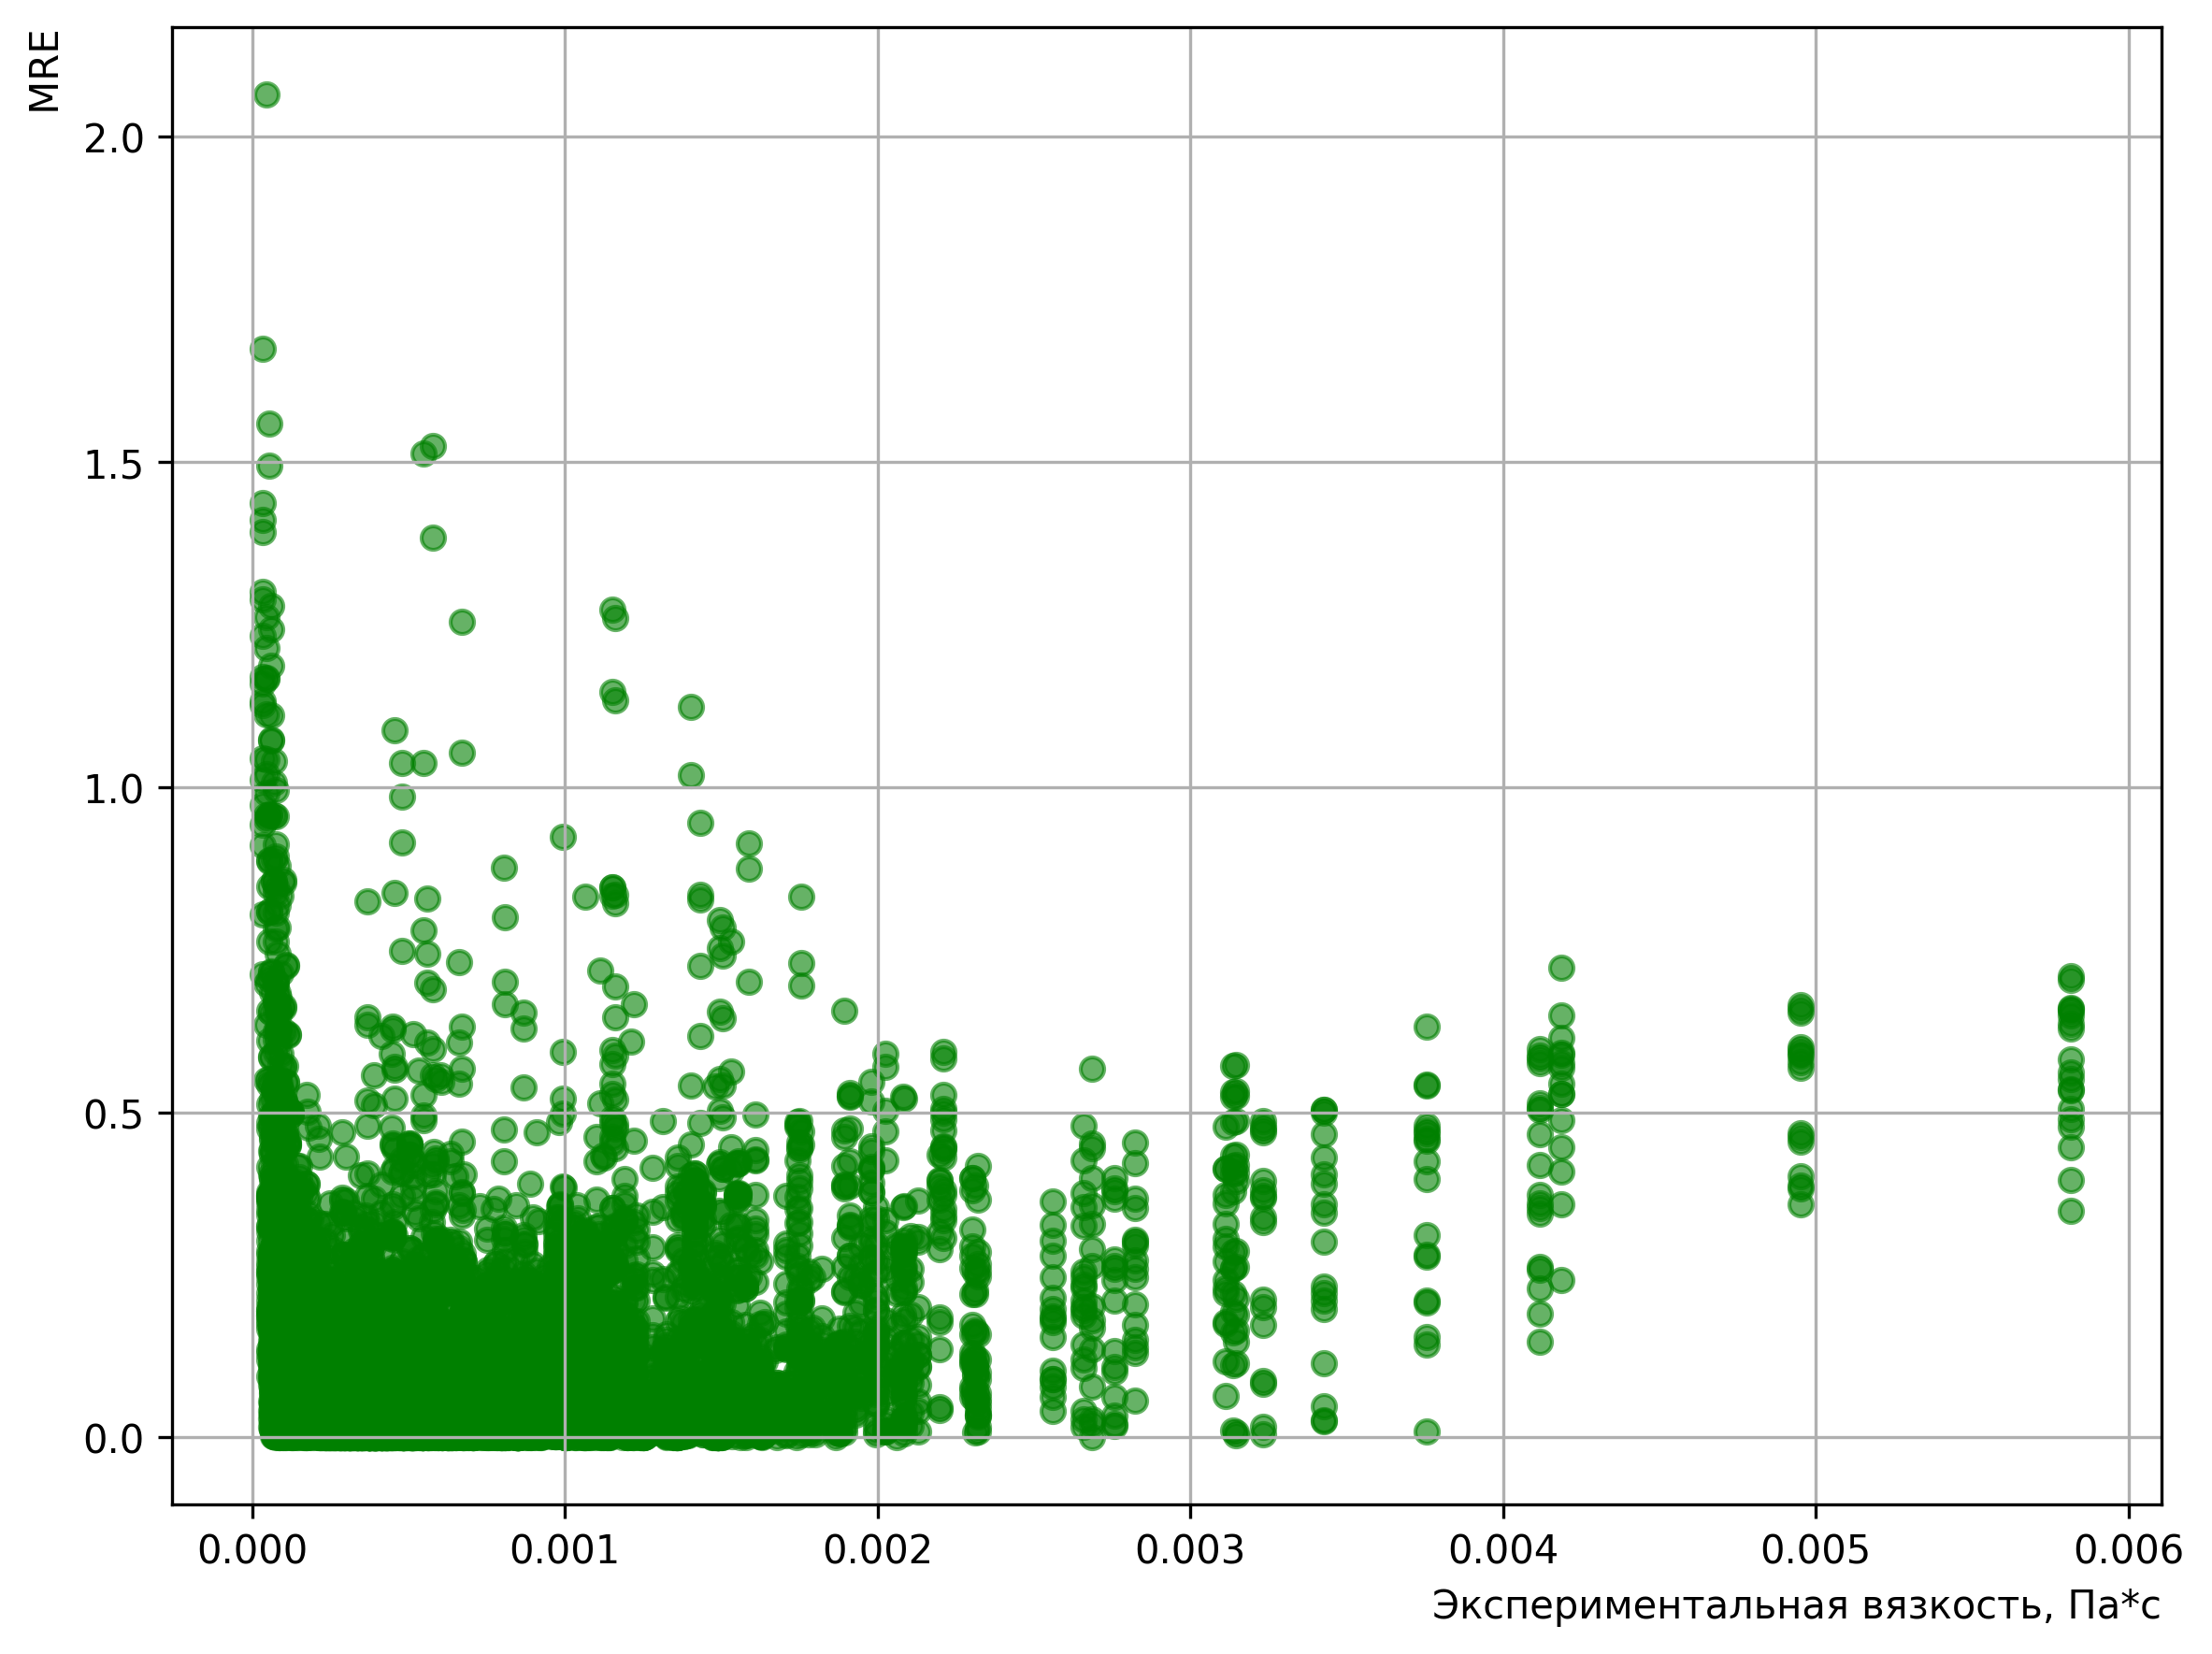
\includegraphics[width=\linewidth]{knn/MRE_KNN (k=3)_0.8_base.png}
            \caption{Относительная ошибка}
        \end{subfigure}
        \caption{Зависимость ошибки модели KNN от истинных значений вязкости. Базовый набор данных, малая обучающая выборка.}
        \label{fig:knn_errors_08_base}
      \end{figure}
      
      \begin{minipage}{\textwidth}
        \textbf{Метрики качества (базовые признаки, обучающая выборка 20\%):}
        \begin{itemize}
          \item RMSE: \( 1.78 \times 10^{-4} \) Па·с;
          \item MAE: \( 4.95 \times 10^{-5} \) Па·с;
          \item MRE: \( 0.0658 \).
        \end{itemize}
      \end{minipage}

    \subsubsection{Влияние расширенных признаков}

      Для проверки, может ли расширенный набор признаков (сгенерированные комбинации и трансформации) улучшить точность в условиях малого числа обучающих данных, модель была протестирована при тех же условиях, но с новым набором признаков. Качество предсказаний немного выросло, но всё ещё не достигло уровня, наблюдаемого при большом тренировочном наборе.
      
      \begin{figure}[ht!]
        \centering
        \begin{subfigure}{0.48\textwidth}
            \centering
            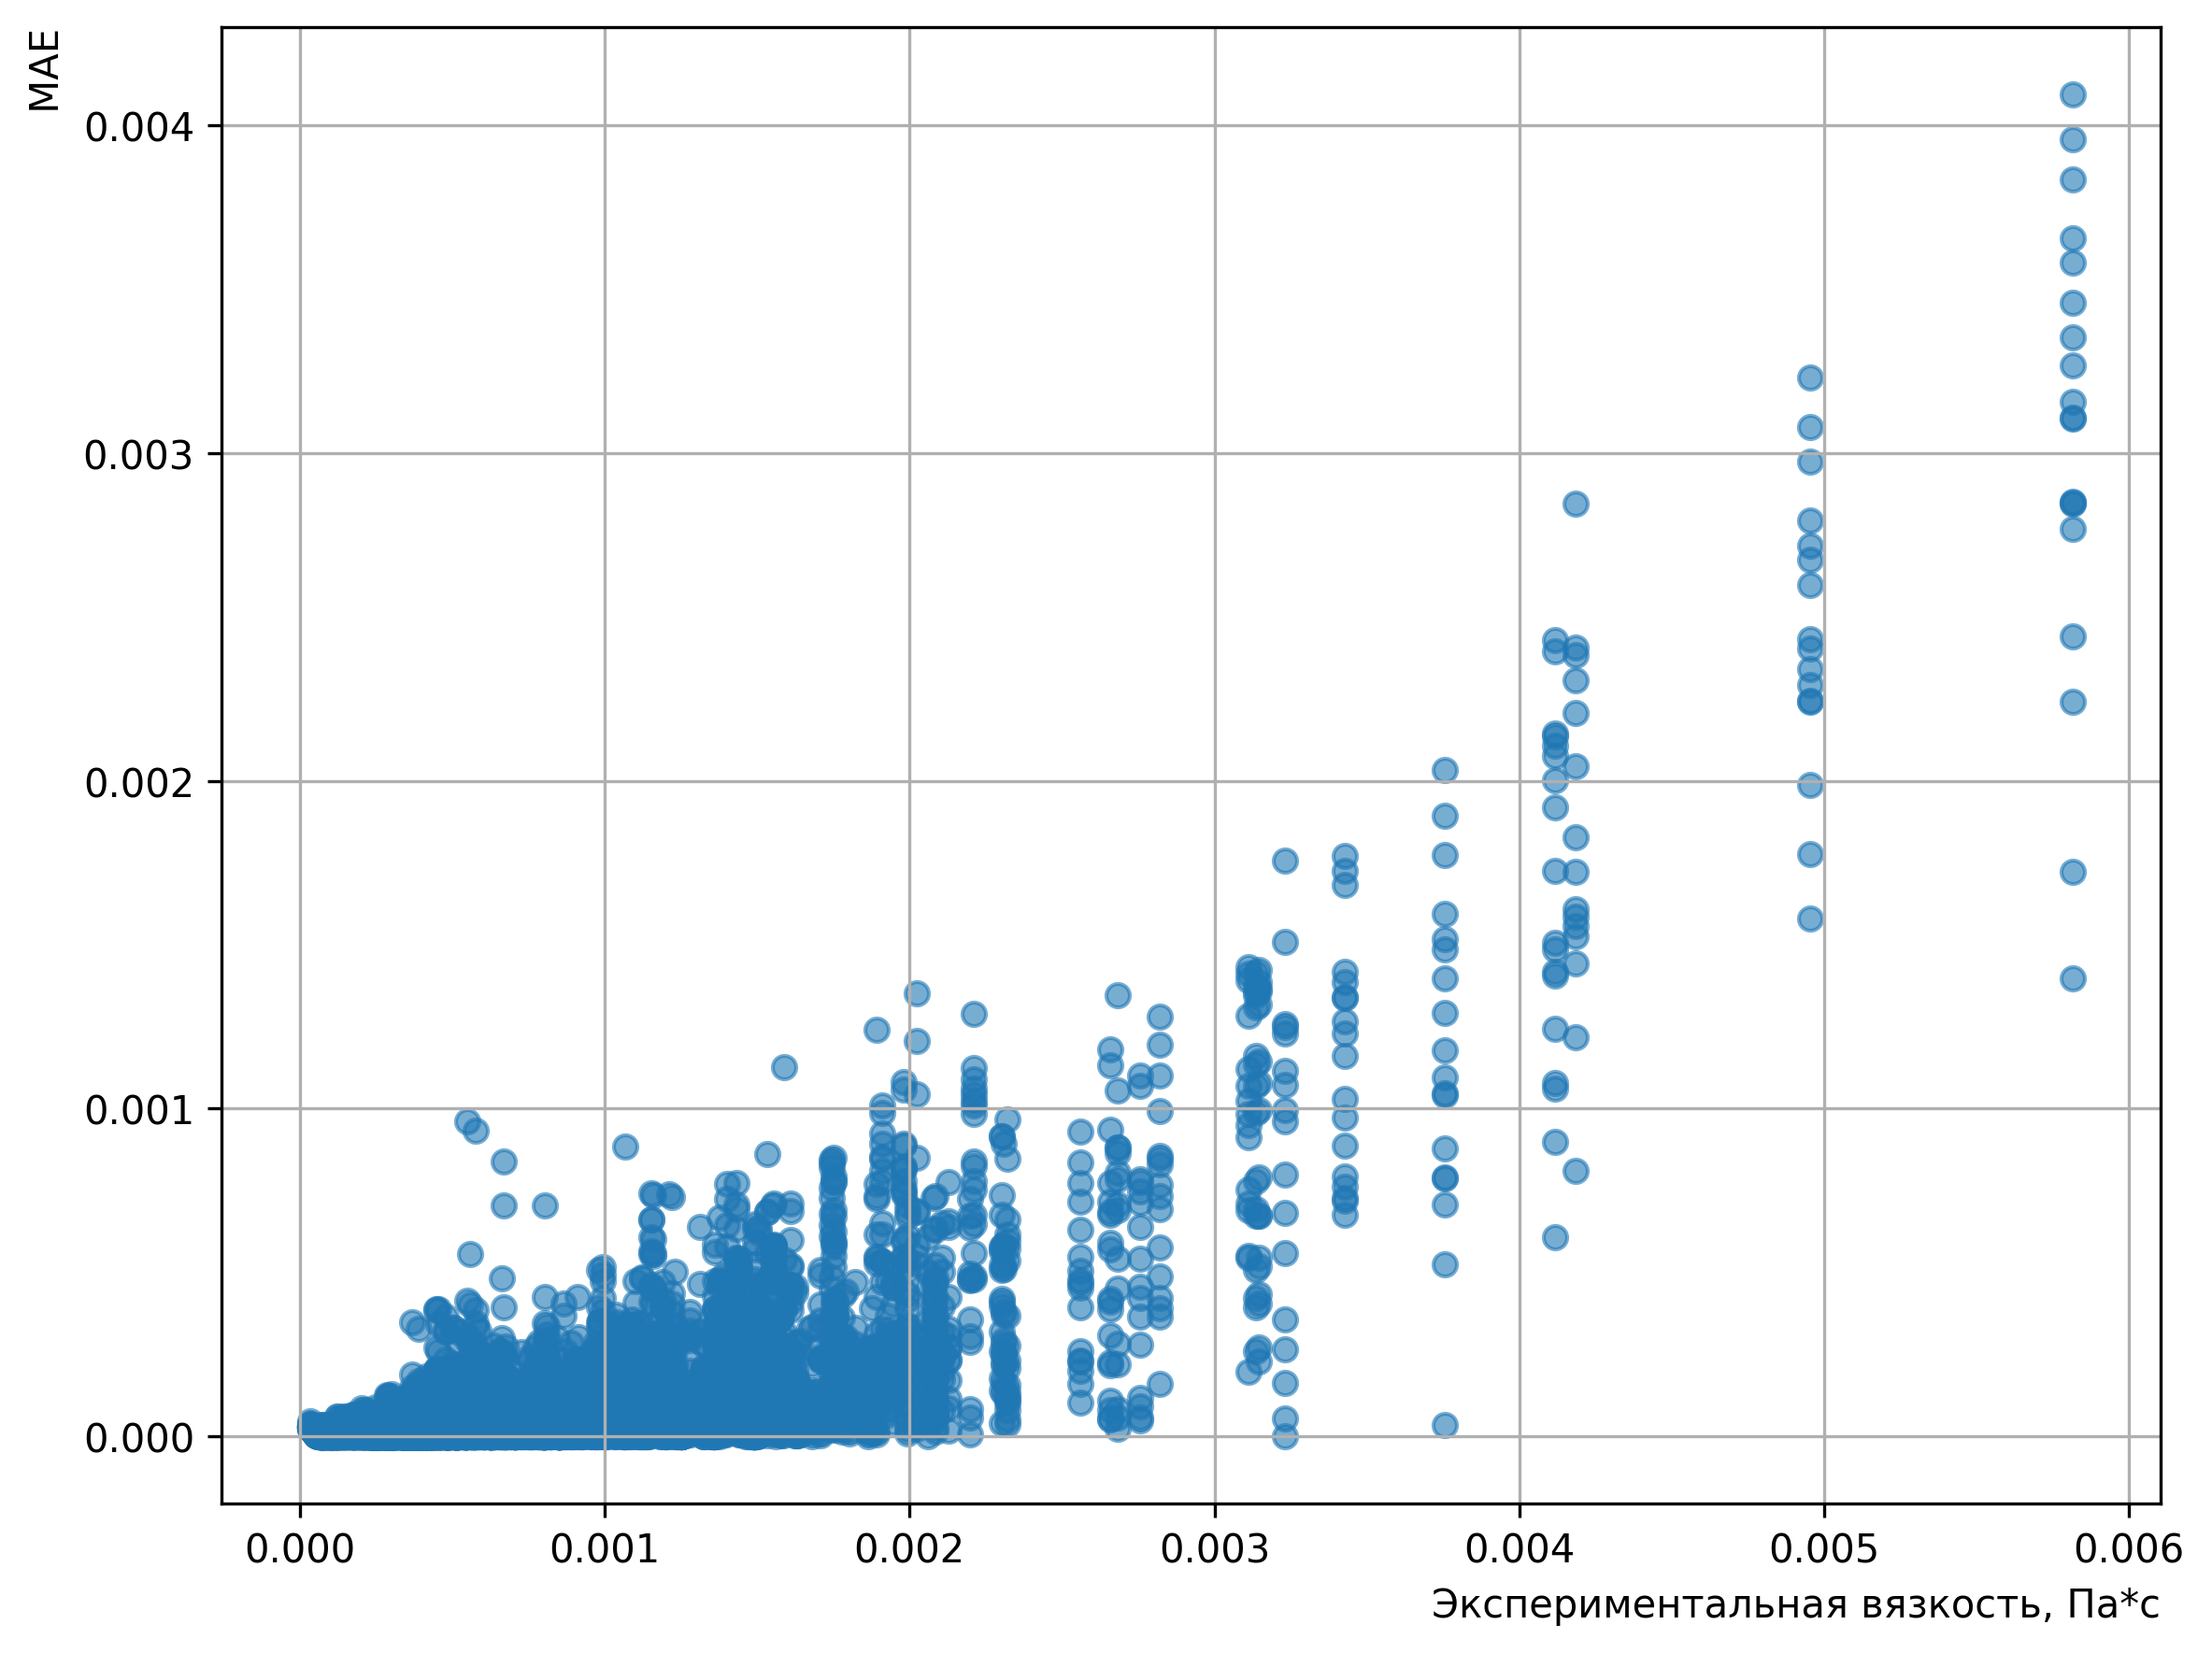
\includegraphics[width=\linewidth]{knn/MAE_KNN (k=3)_0.8_rules.png}
            \caption{Абсолютная ошибка}
        \end{subfigure}
        \hfill
        \begin{subfigure}{0.48\textwidth}
            \centering
            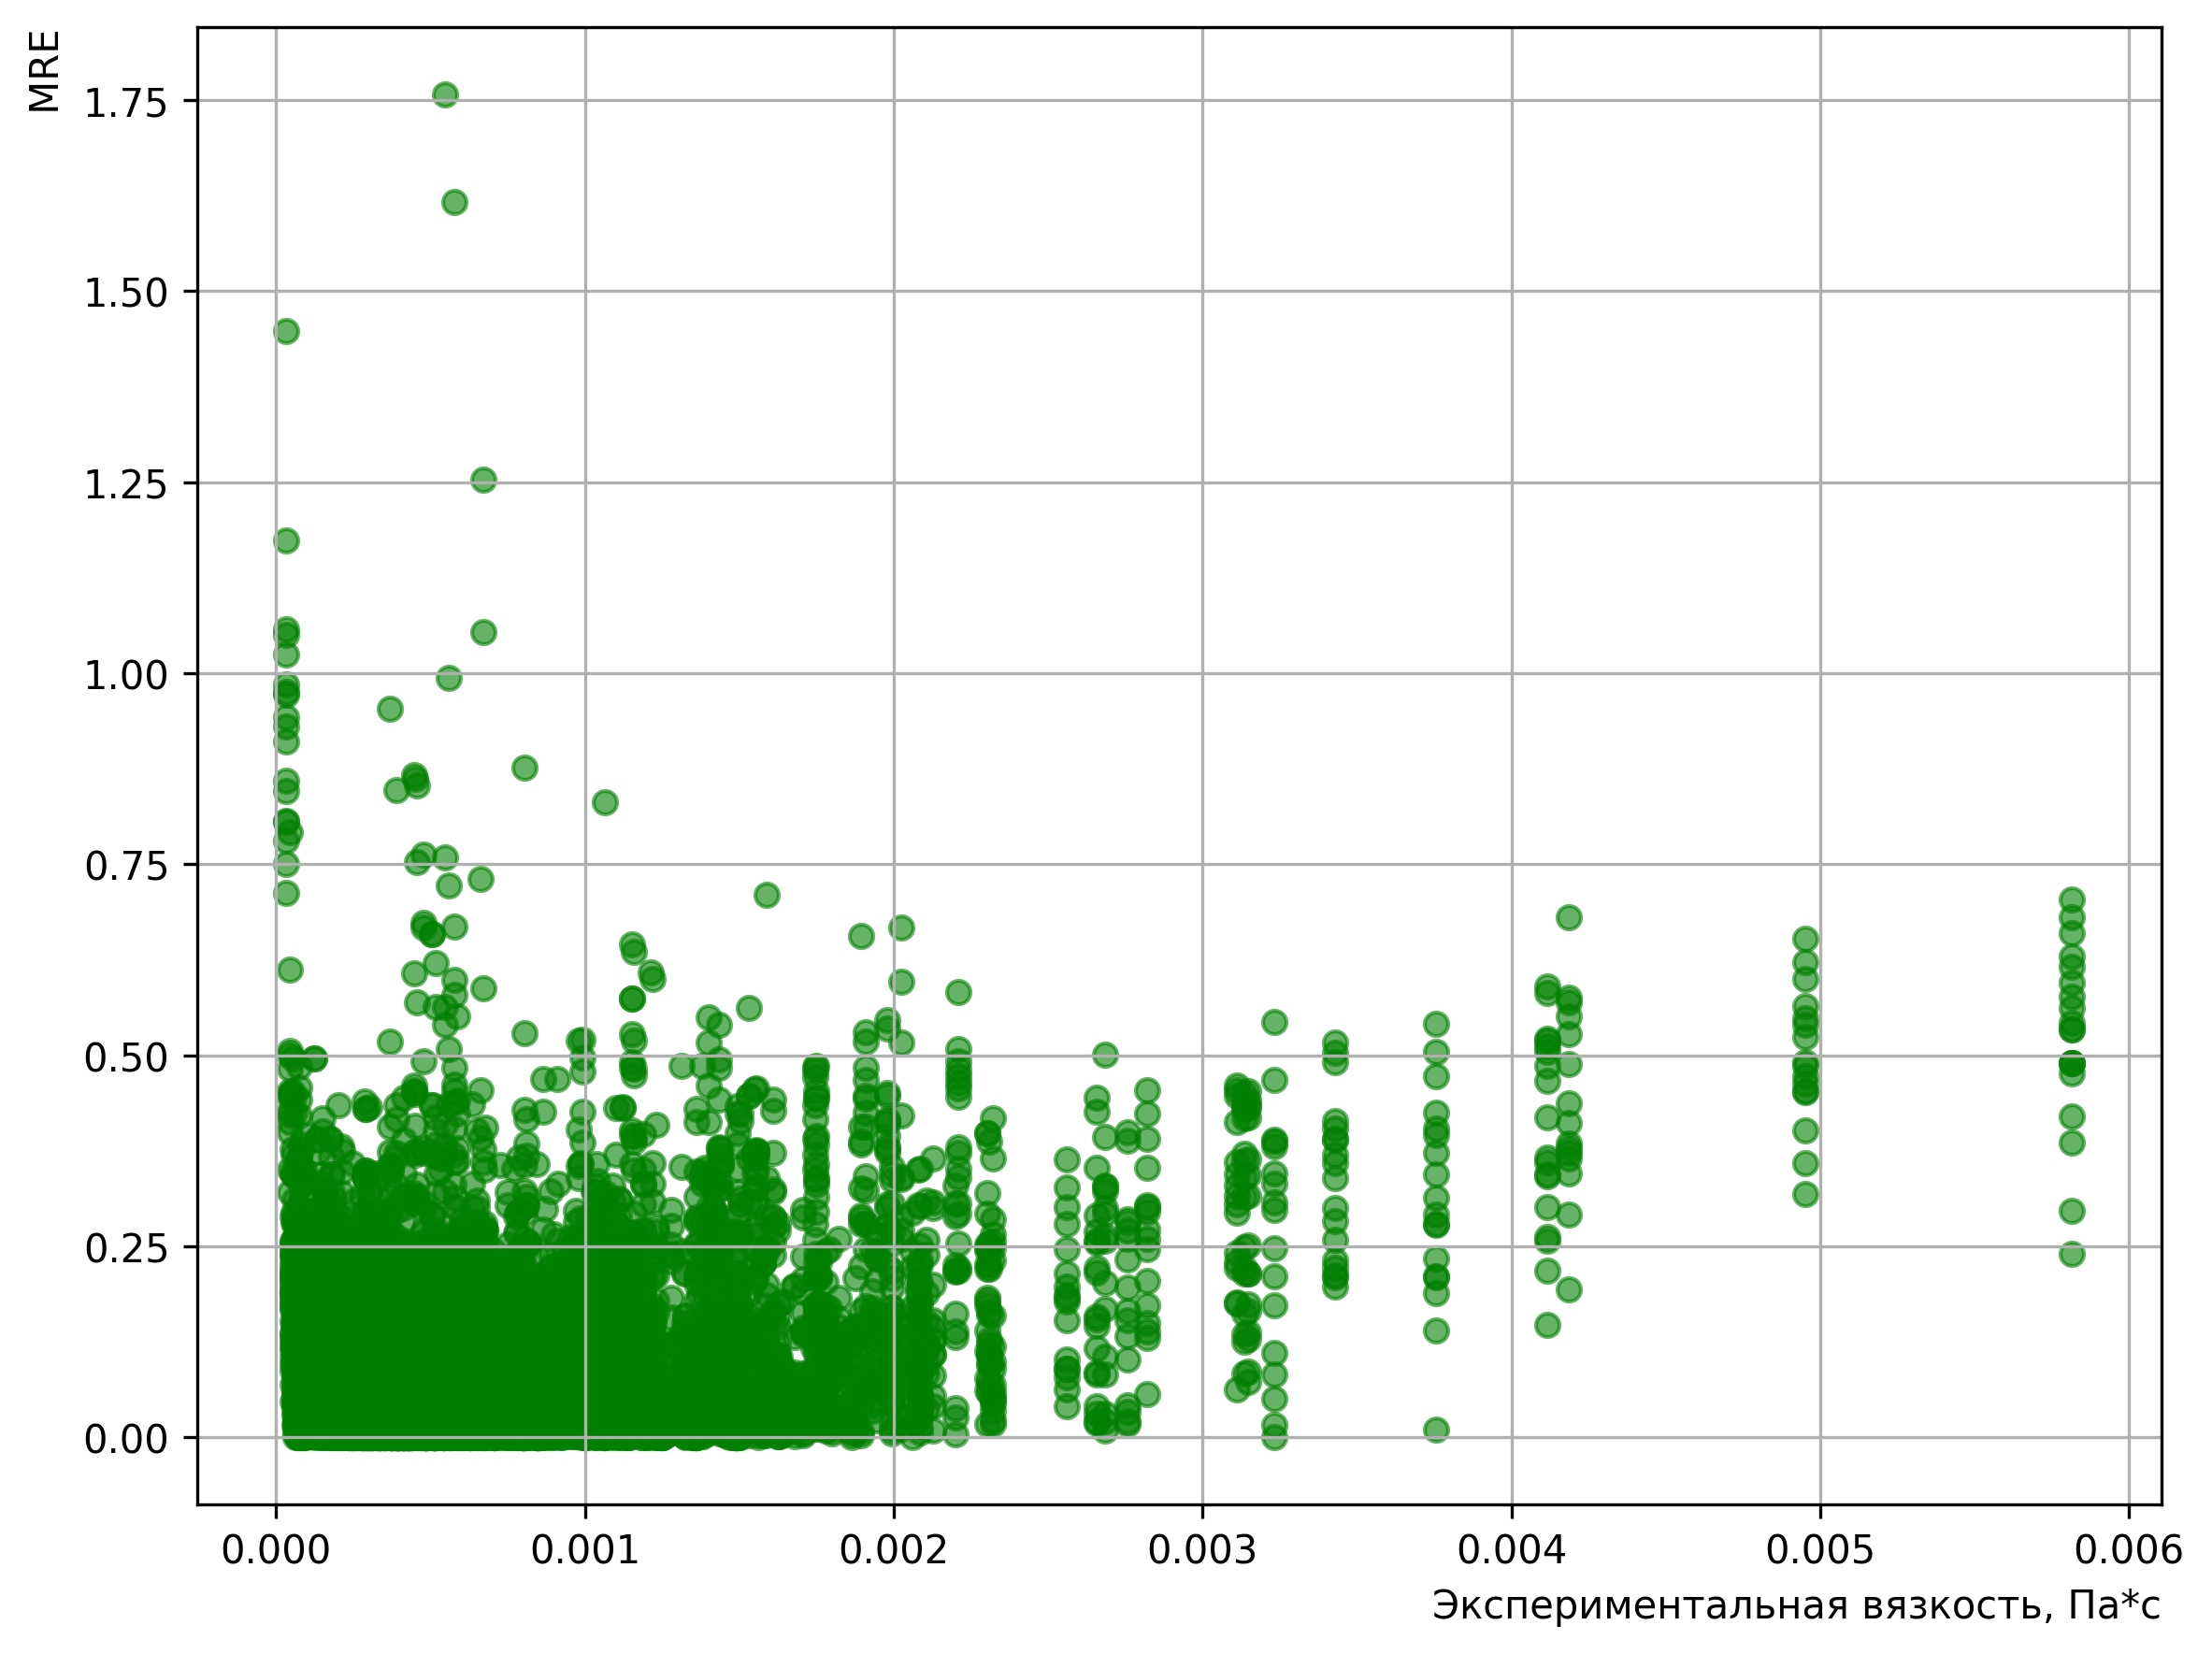
\includegraphics[width=\linewidth]{knn/MRE_KNN (k=3)_0.8_rules.png}
            \caption{Относительная ошибка}
        \end{subfigure}
        \caption{Зависимость ошибки модели KNN от истинных значений вязкости. Расширенный набор данных, малая обучающая выборка.}
        \label{fig:knn_errors_08_rules}
      \end{figure}

      \begin{minipage}{\textwidth}
        \textbf{Метрики качества (расширенные признаки, обучающая выборка 20\%):}
        \begin{itemize}
          \item RMSE: \( 1.62 \times 10^{-4} \) Па·с;
          \item MAE: \( 4.65 \times 10^{-5} \) Па·с;
          \item MRE: \( 0.0594 \).
        \end{itemize}
      \end{minipage}

    \subsubsection{Вывод по методу KNN}

      Модель KNN ожидаемо показала хорошую точность на обучающих данных и слабую обобщающую способность. Это подтверждает предположение, что метод плохо переносится на новые области пространства признаков. Использование расширенных признаков позволило немного улучшить результаты, но не устранило фундаментальные ограничения метода. KNN может использоваться как базовая оценка и для валидации корректности данных, но не подходит в качестве основной модели для задач обобщения и предсказания вязкости по параметрам вещества.


  \subsection{Случайный лес}

    Модель случайного леса относится к ансамблевым методам машинного обучения и строится на объединении большого количества решающих деревьев. В отличие от метода ближайших соседей, который делает предсказания, опираясь исключительно на локальные участки пространства признаков, случайный лес формирует обобщённые предсказания, агрегируя решения деревьев, обученных на разных подмножествах данных. Благодаря этому, модель хорошо справляется с задачами регрессии в условиях сложных нелинейных зависимостей между признаками.
    
    В данной работе использовалась реализация \texttt{RandomForestRegressor} из библиотеки \texttt{sklearn.ensemble}. Модель тестировалась с базовыми параметрами по умолчанию (\( n\_estimators = 100 \) и др.), так как изменение настроек не приводило к устойчивому улучшению качества, а в отдельных случаях даже снижало точность.
    
    \subsubsection{Оценка точности на большом обучающем наборе}
    
    При обучении модели на 80\% данных и использовании только базовых признаков случайный лес показал хорошие результаты. По сравнению с методом ближайших соседей, была достигнута существенно более высокая точность, особенно по RMSE и MAE, хотя значения относительной ошибки оставались сравнимыми. Результаты представлены на рисунке~\autoref{fig:random_forest_errors_02_base}.
    
    \begin{figure}[ht!]
      \centering
      \begin{subfigure}{0.48\textwidth}
          \centering
          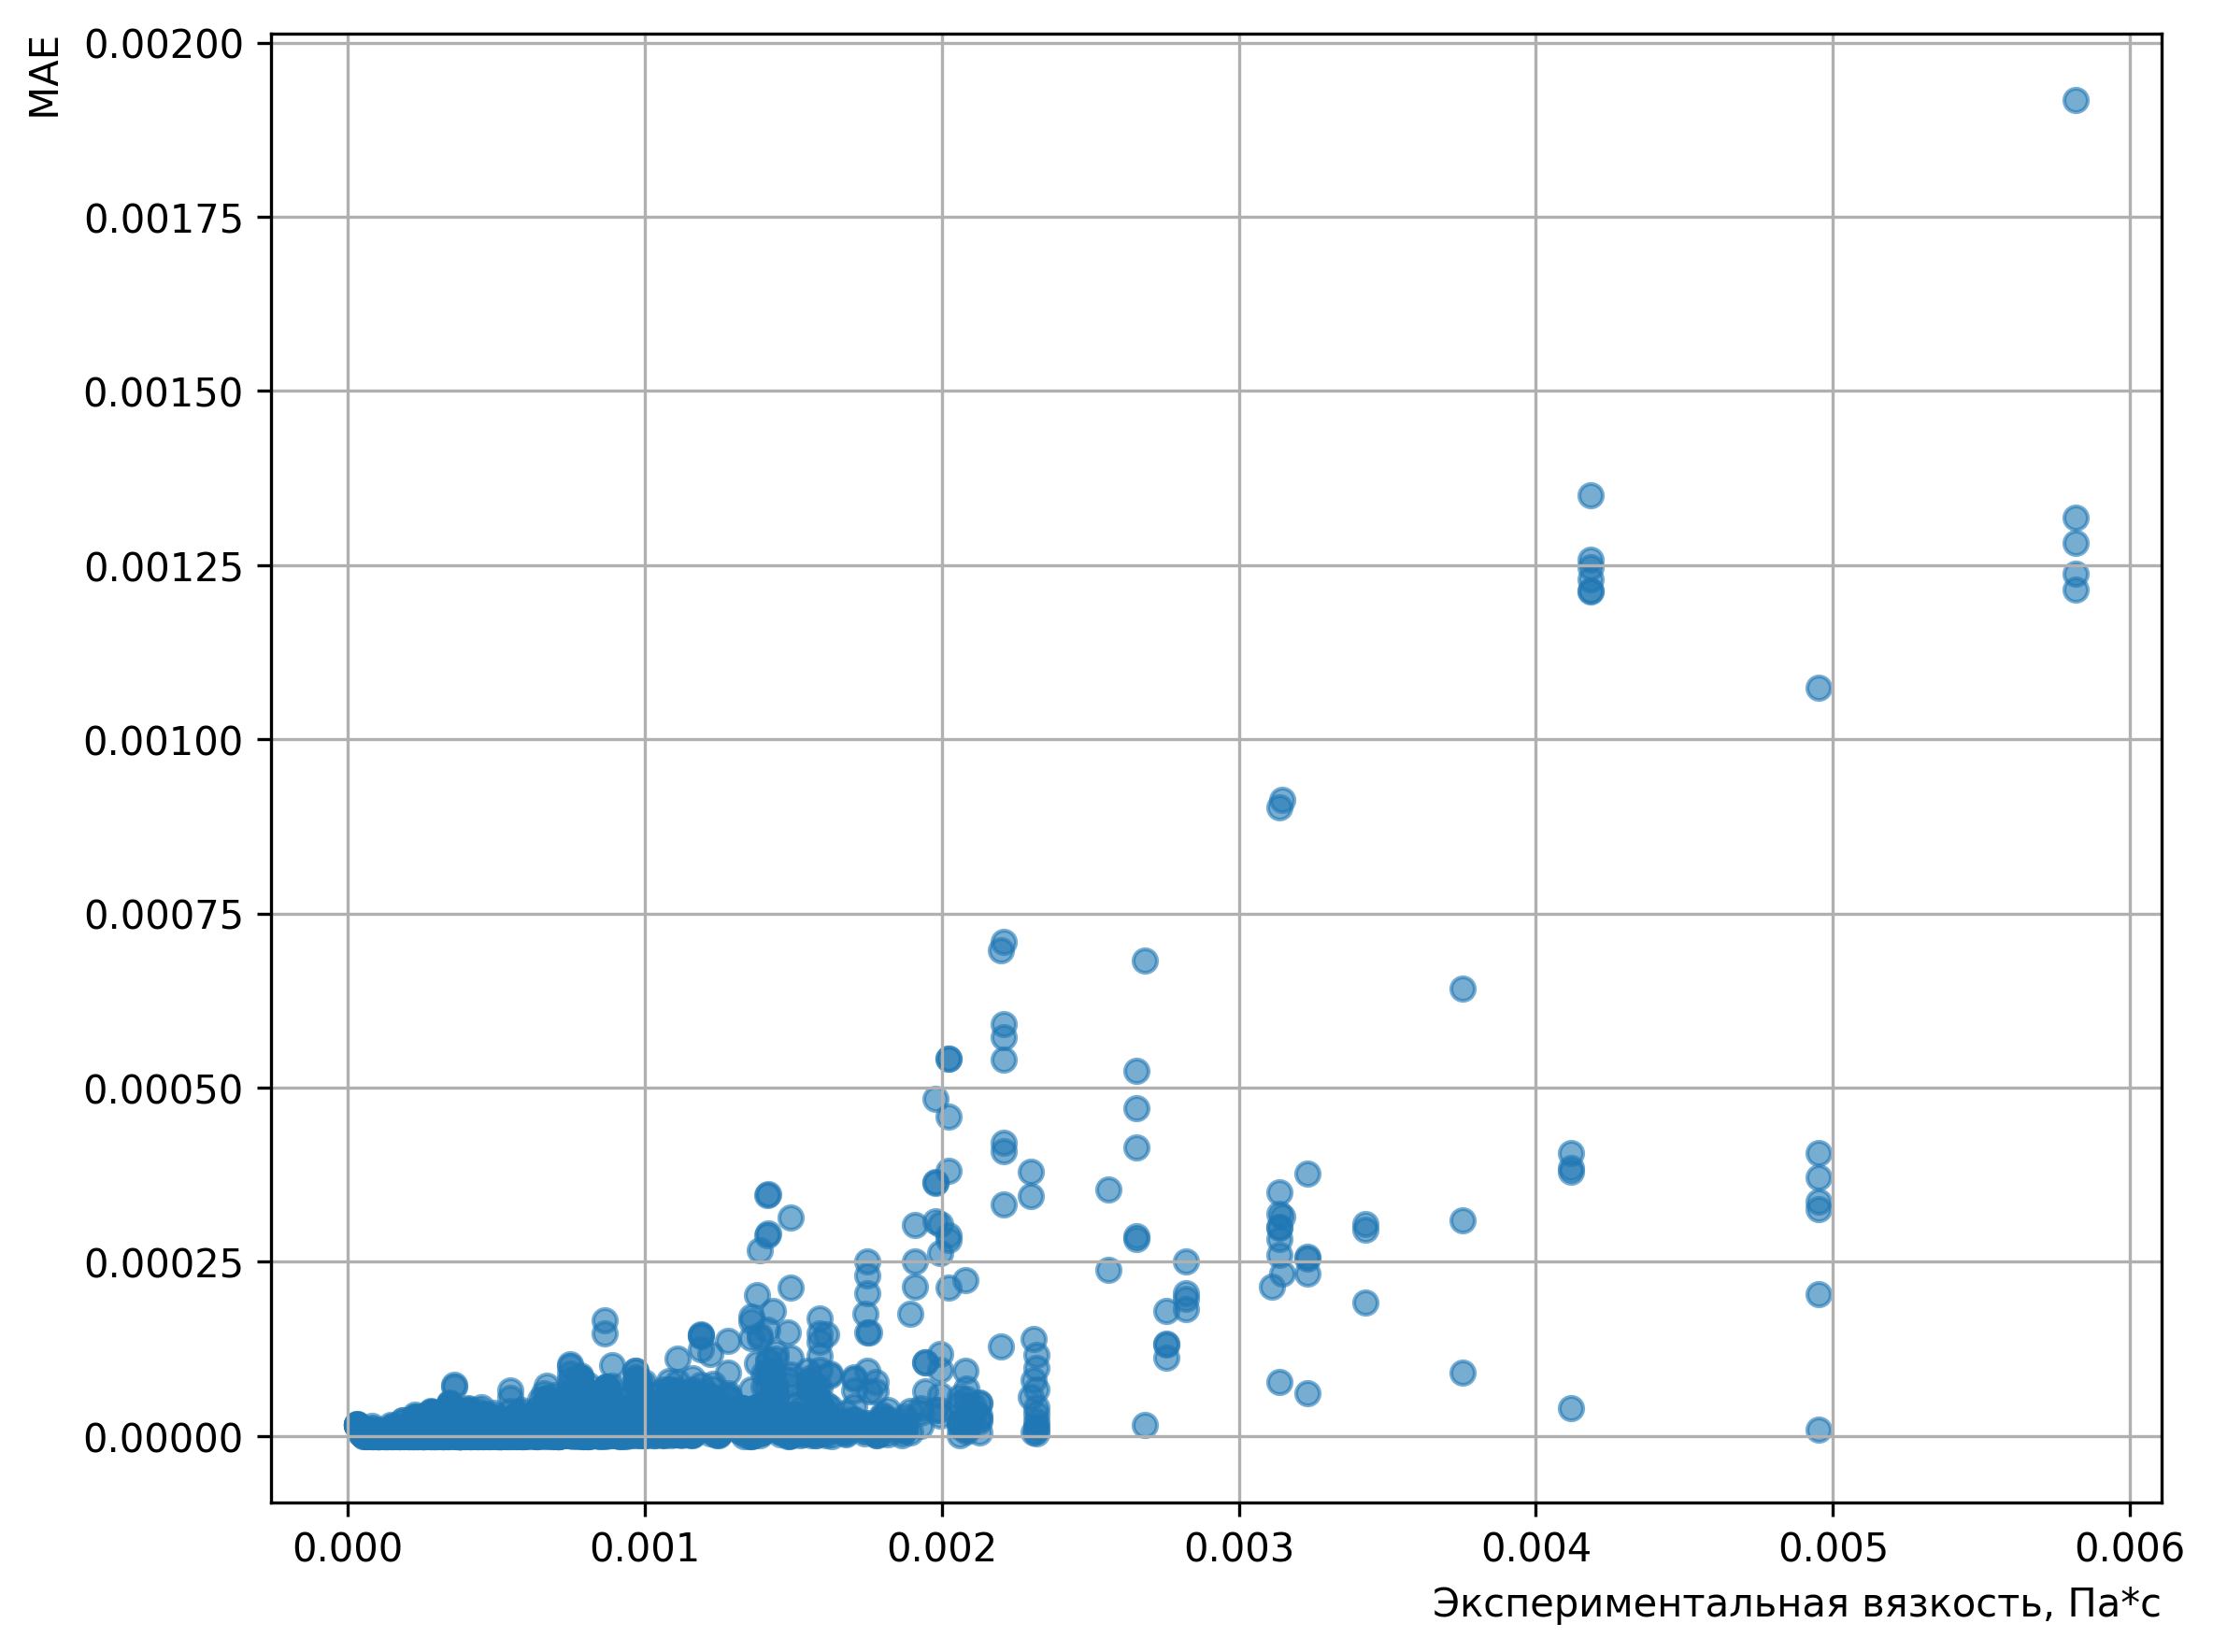
\includegraphics[width=\linewidth]{random_forest/MAE_Random Forest Model_0.2_base.png}
          \caption{Абсолютная ошибка}
      \end{subfigure}
      \hfill
      \begin{subfigure}{0.48\textwidth}
          \centering
          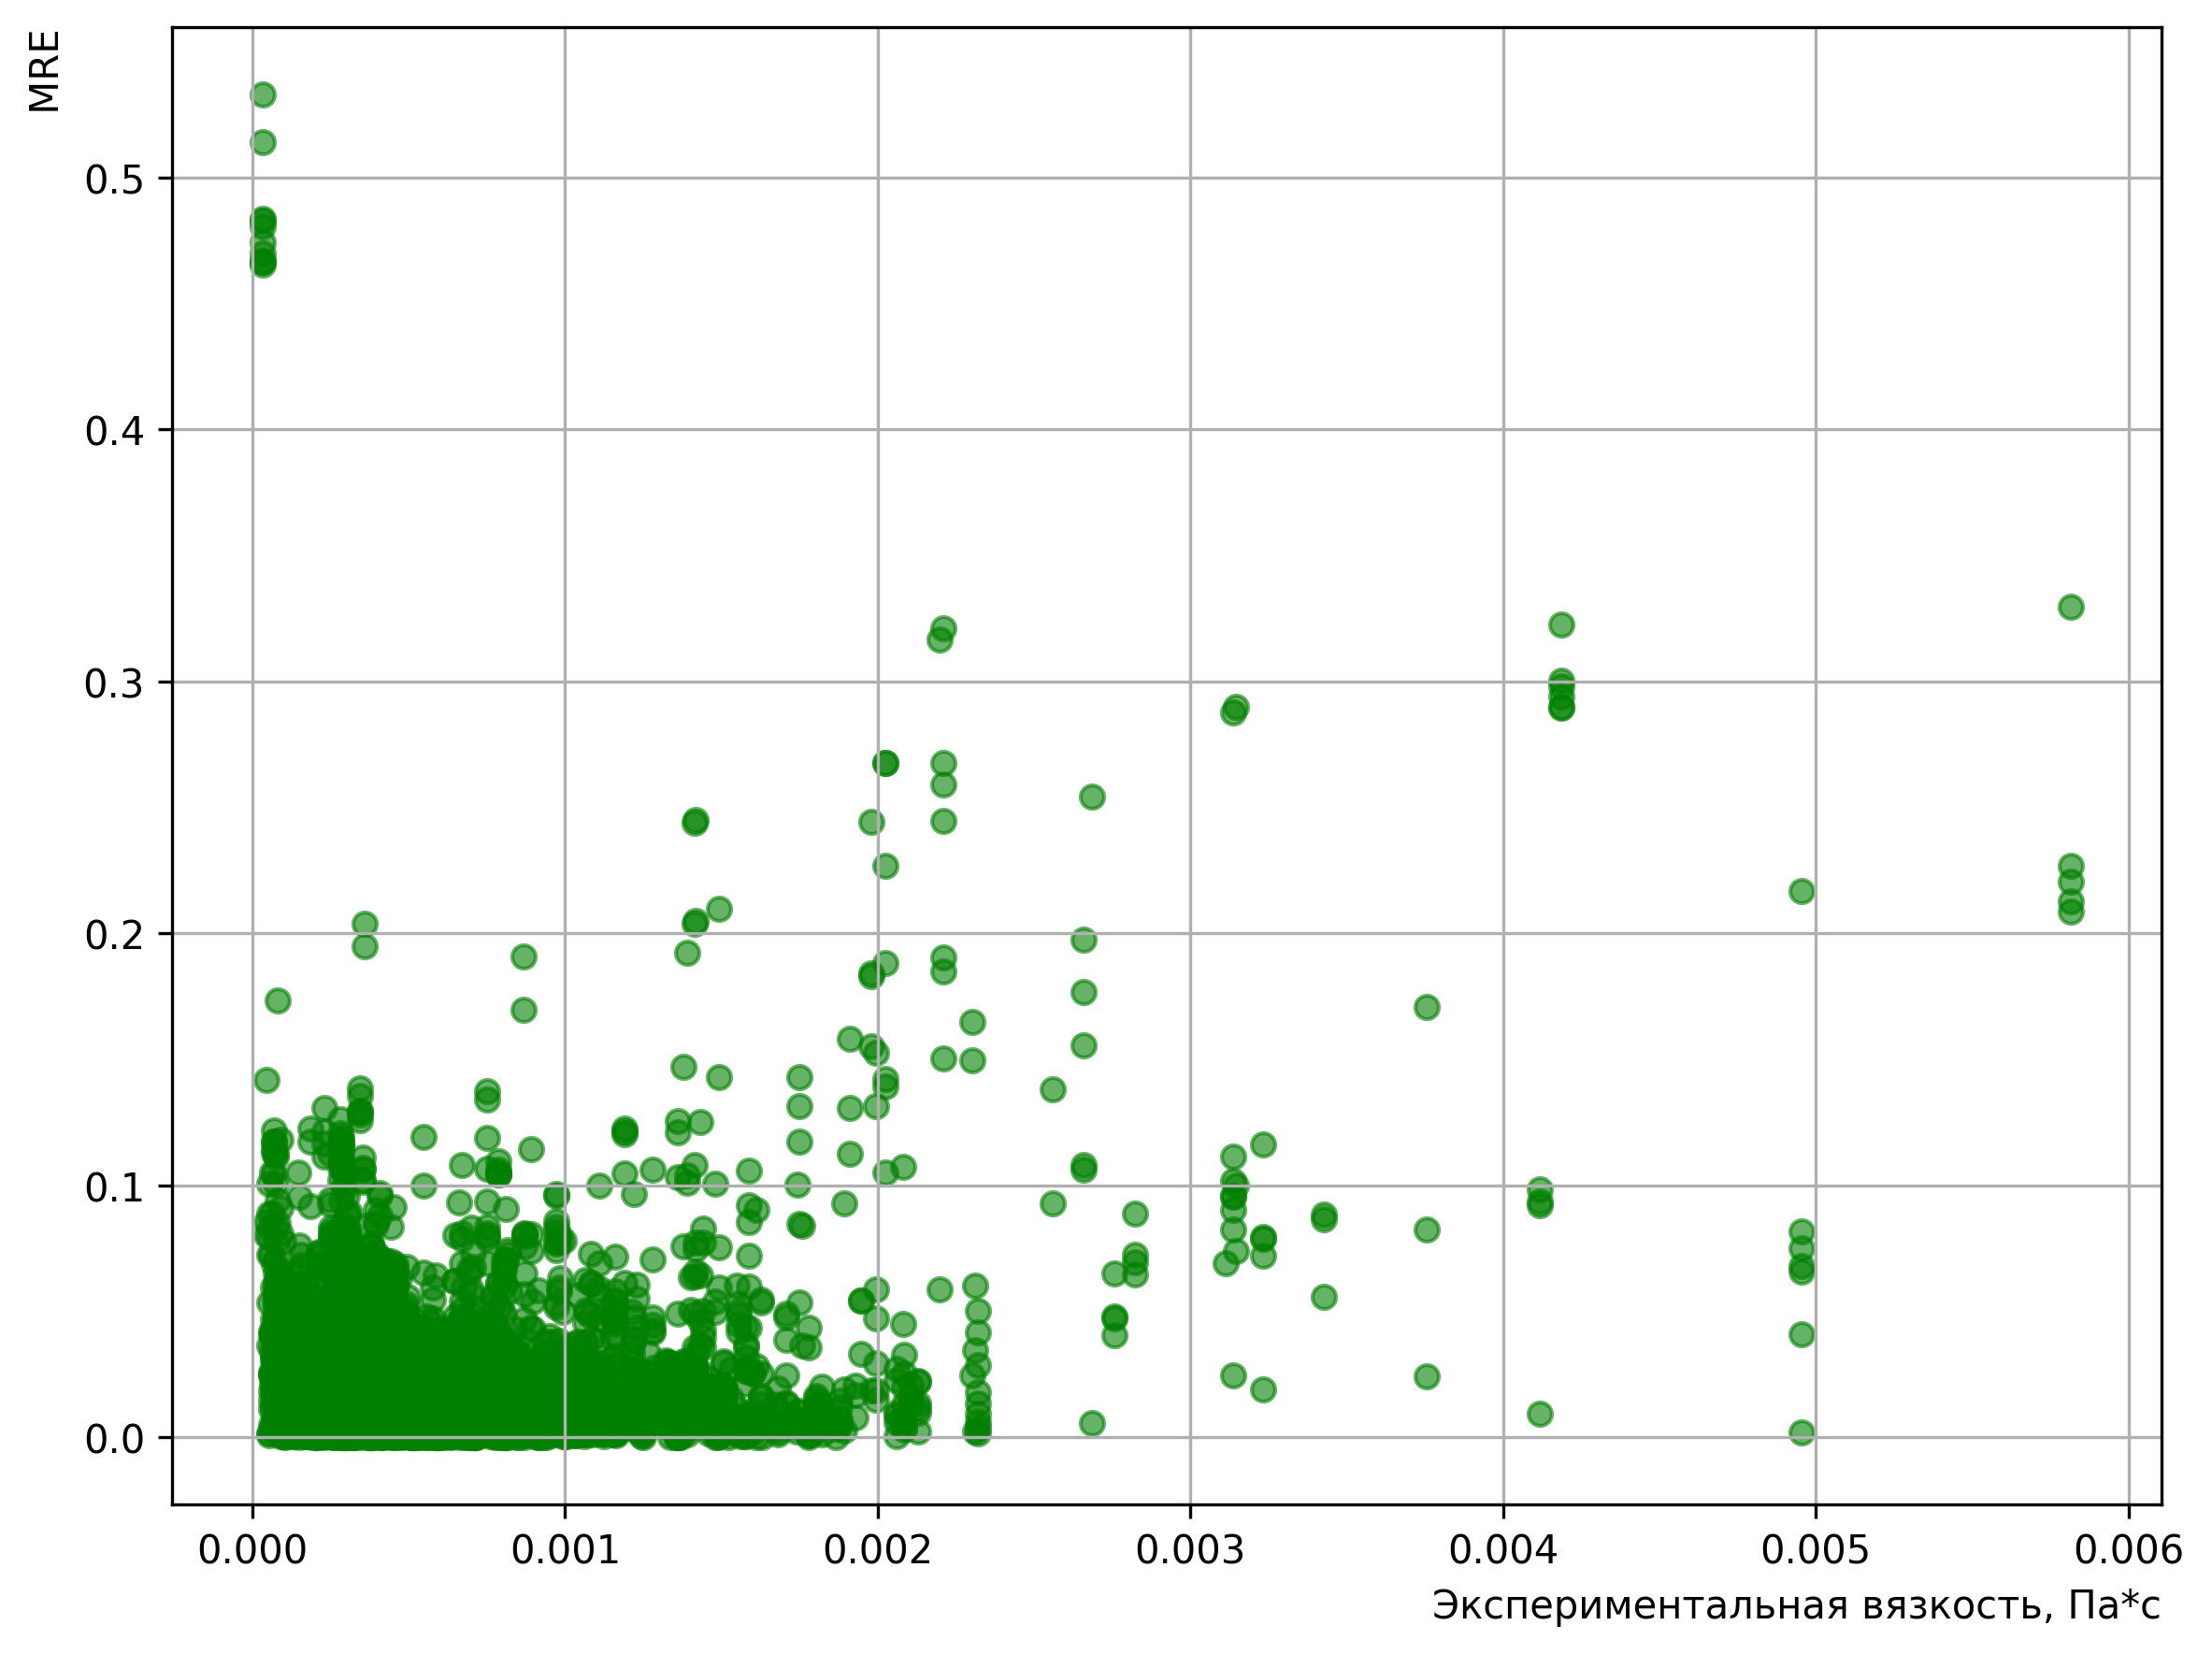
\includegraphics[width=\linewidth]{random_forest/MRE_Random Forest Model_0.2_base.png}
          \caption{Относительная ошибка}
      \end{subfigure}
      \caption{Зависимость ошибки модели случайного леса от истинных значений вязкости. Базовый набор признаков, большая обучающая выборка.}
      \label{fig:random_forest_errors_02_base}
    \end{figure}
    
    \begin{minipage}{\textwidth}
      \textbf{Метрики качества (базовые признаки, обучающая выборка 80\%):}
      \begin{itemize}
          \item RMSE: \( 6.40 \times 10^{-5} \) Па·с;
          \item MAE: \( 1.63 \times 10^{-5} \) Па·с;
          \item MRE: \( 0.0212 \).
      \end{itemize}
    \end{minipage}
    
    \subsubsection{Оценка на ограниченных данных}
    
    Для оценки способности модели обобщать данные была проведена обратная процедура: обучение на 20\% выборки и тестирование на оставшихся 80\%. При этом значения ошибок возросли, как и ожидалось, однако модель сохраняла уверенную точность. Относительная ошибка по-прежнему оставалась ниже 5\%, что свидетельствует о приемлемой обобщающей способности \autoref{fig:random_forest_errors_08_base}.
    
    \begin{figure}[ht!]
      \centering
      \begin{subfigure}{0.48\textwidth}
          \centering
          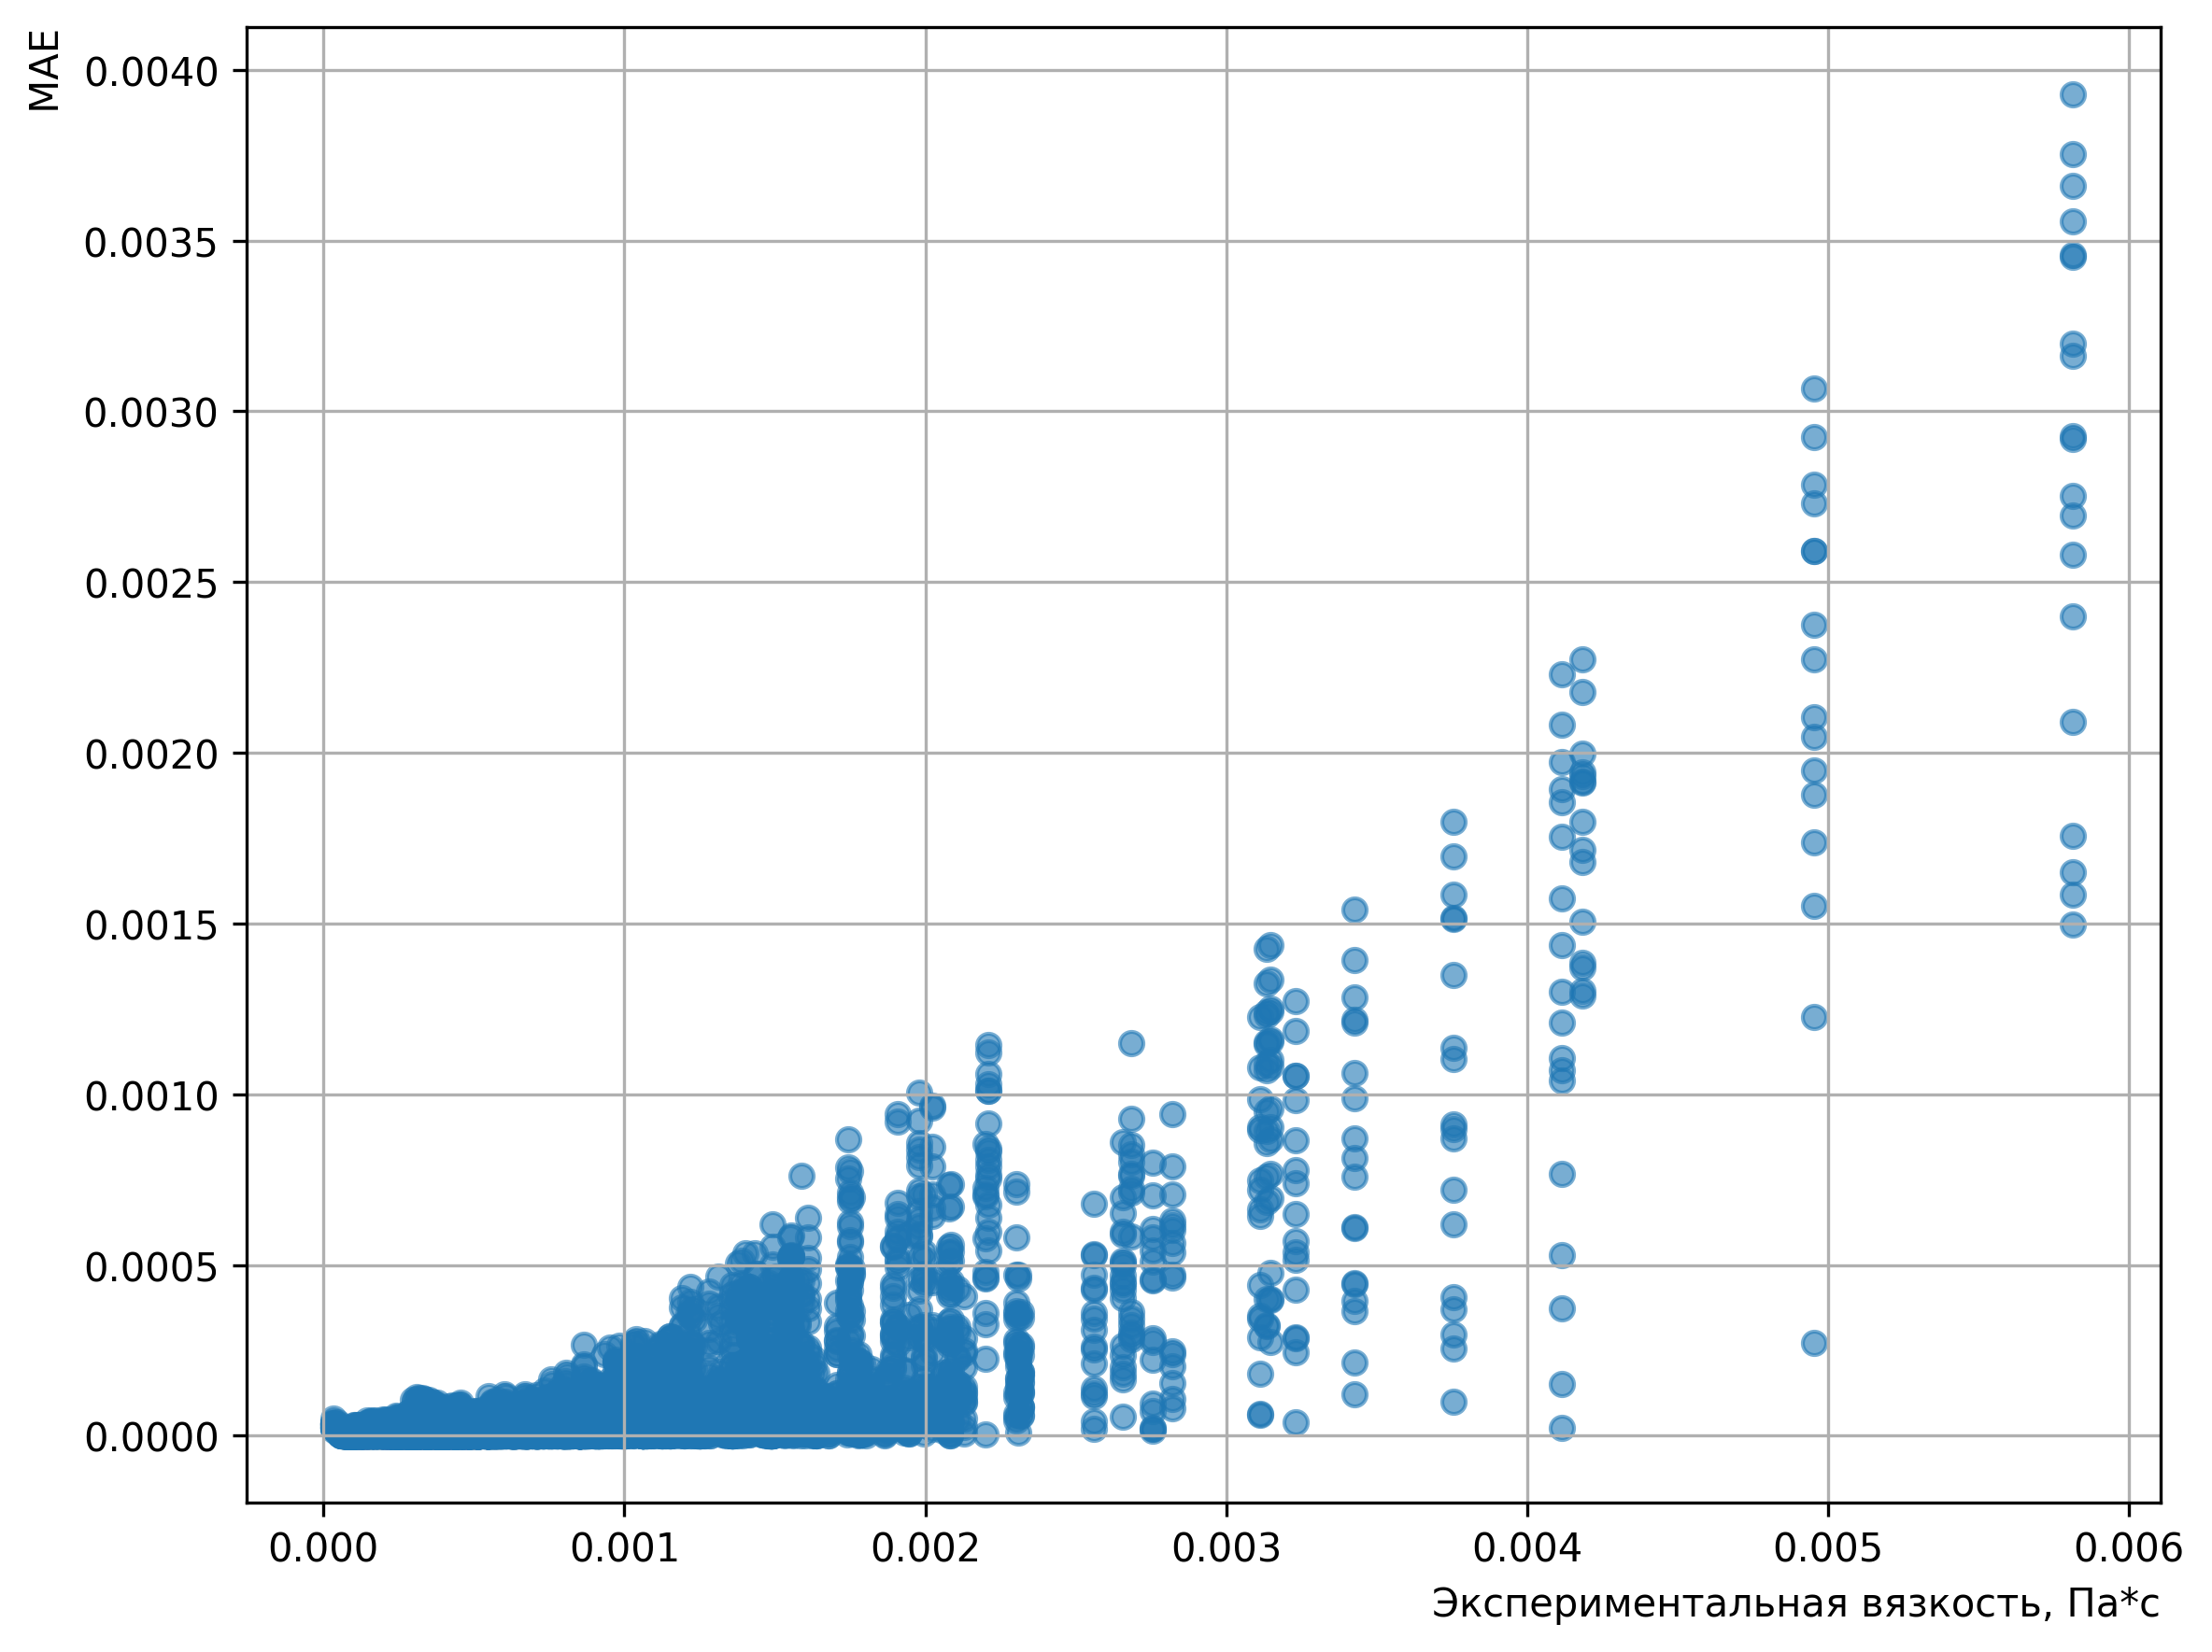
\includegraphics[width=\linewidth]{random_forest/MAE_Random Forest Model_0.8_base.png}
          \caption{Абсолютная ошибка}
      \end{subfigure}
      \hfill
      \begin{subfigure}{0.48\textwidth}
          \centering
          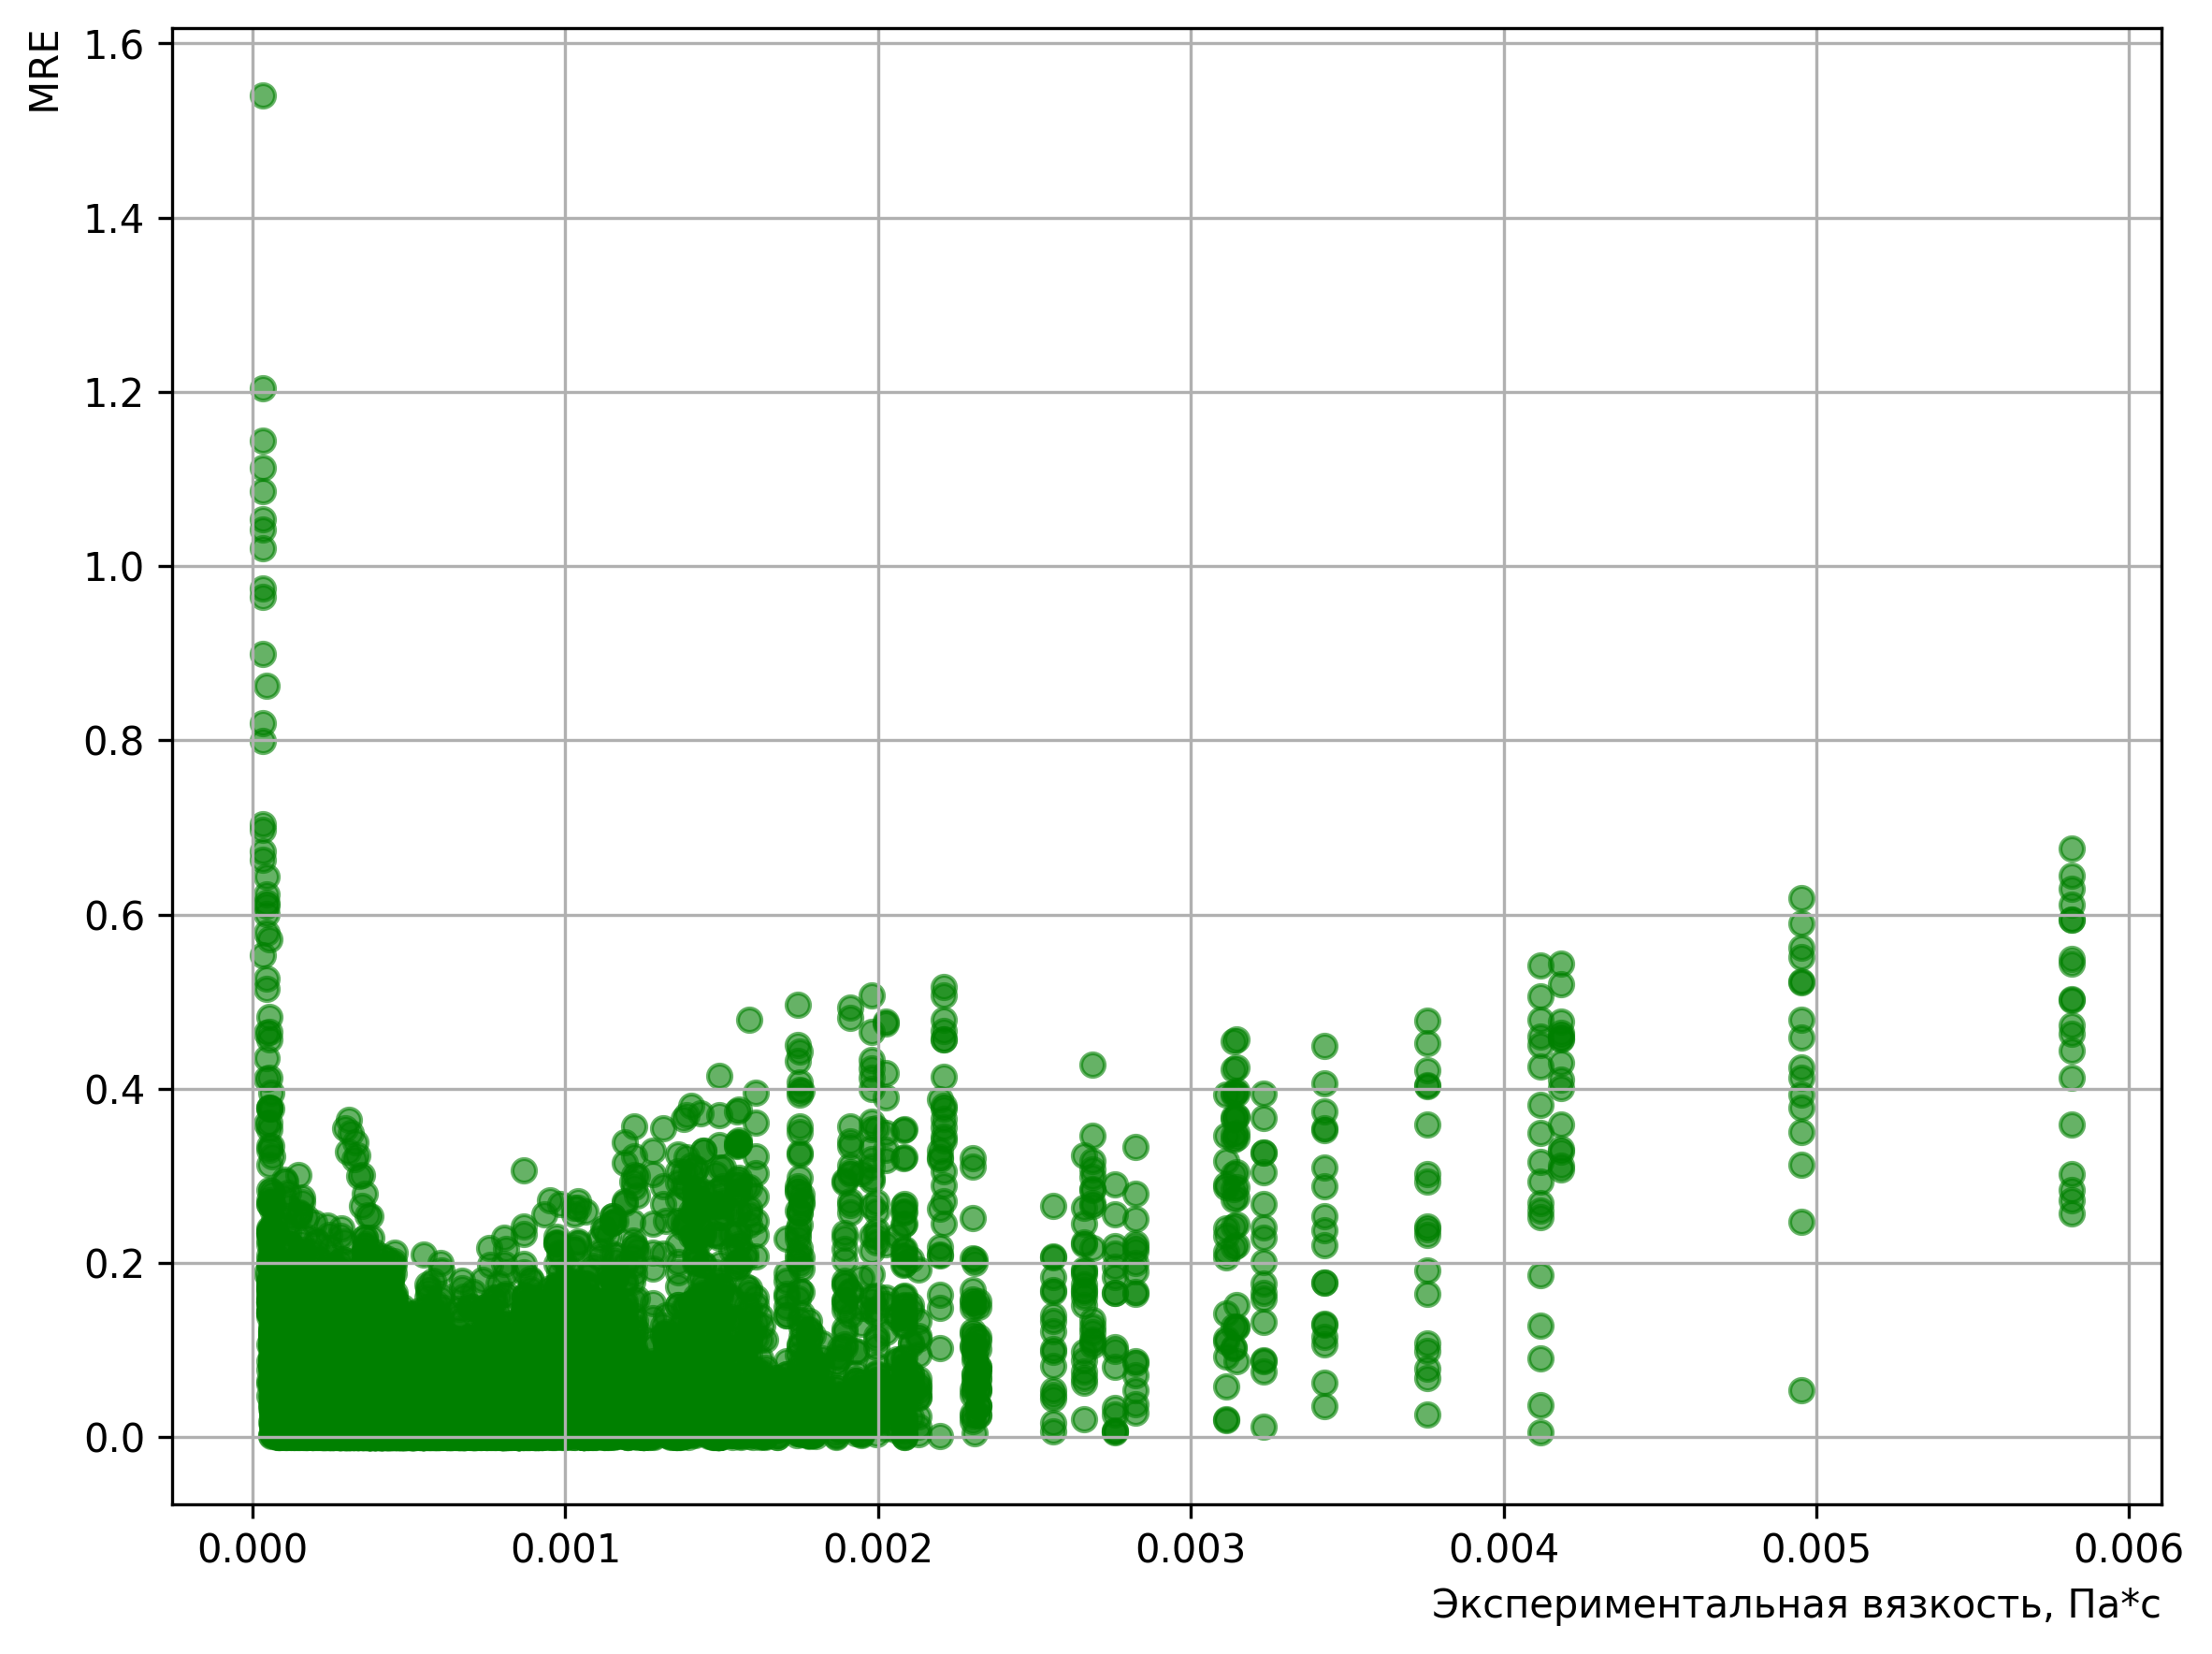
\includegraphics[width=\linewidth]{random_forest/MRE_Random Forest Model_0.8_base.png}
          \caption{Относительная ошибка}
      \end{subfigure}
      \caption{Зависимость ошибки модели случайного леса от истинных значений вязкости. Базовый набор признаков, малая обучающая выборка.}
      \label{fig:random_forest_errors_08_base}
    \end{figure}
    
    \begin{minipage}{\textwidth}
    \textbf{Метрики качества (базовые признаки, обучающая выборка 20\%):}
      \begin{itemize}
          \item RMSE: \( 1.36 \times 10^{-4} \) Па·с;
          \item MAE: \( 3.22 \times 10^{-5} \) Па·с;
          \item MRE: \( 0.0390 \).
      \end{itemize}
    \end{minipage}
    
    \subsubsection{Влияние расширенных признаков}
    
    Далее была проверена эффективность модели на расширенном наборе признаков, включающем автоматически сгенерированные комбинации и преобразования. Обучение вновь проводилось на 20\% выборки. Результаты показали, что такие признаки действительно улучшают качество предсказания: значения всех ошибок снизились по сравнению с базовым вариантом \autoref{fig:random_forest_errors_08_rules}.
    
    \begin{figure}[ht!]
      \centering
      \begin{subfigure}{0.48\textwidth}
          \centering
          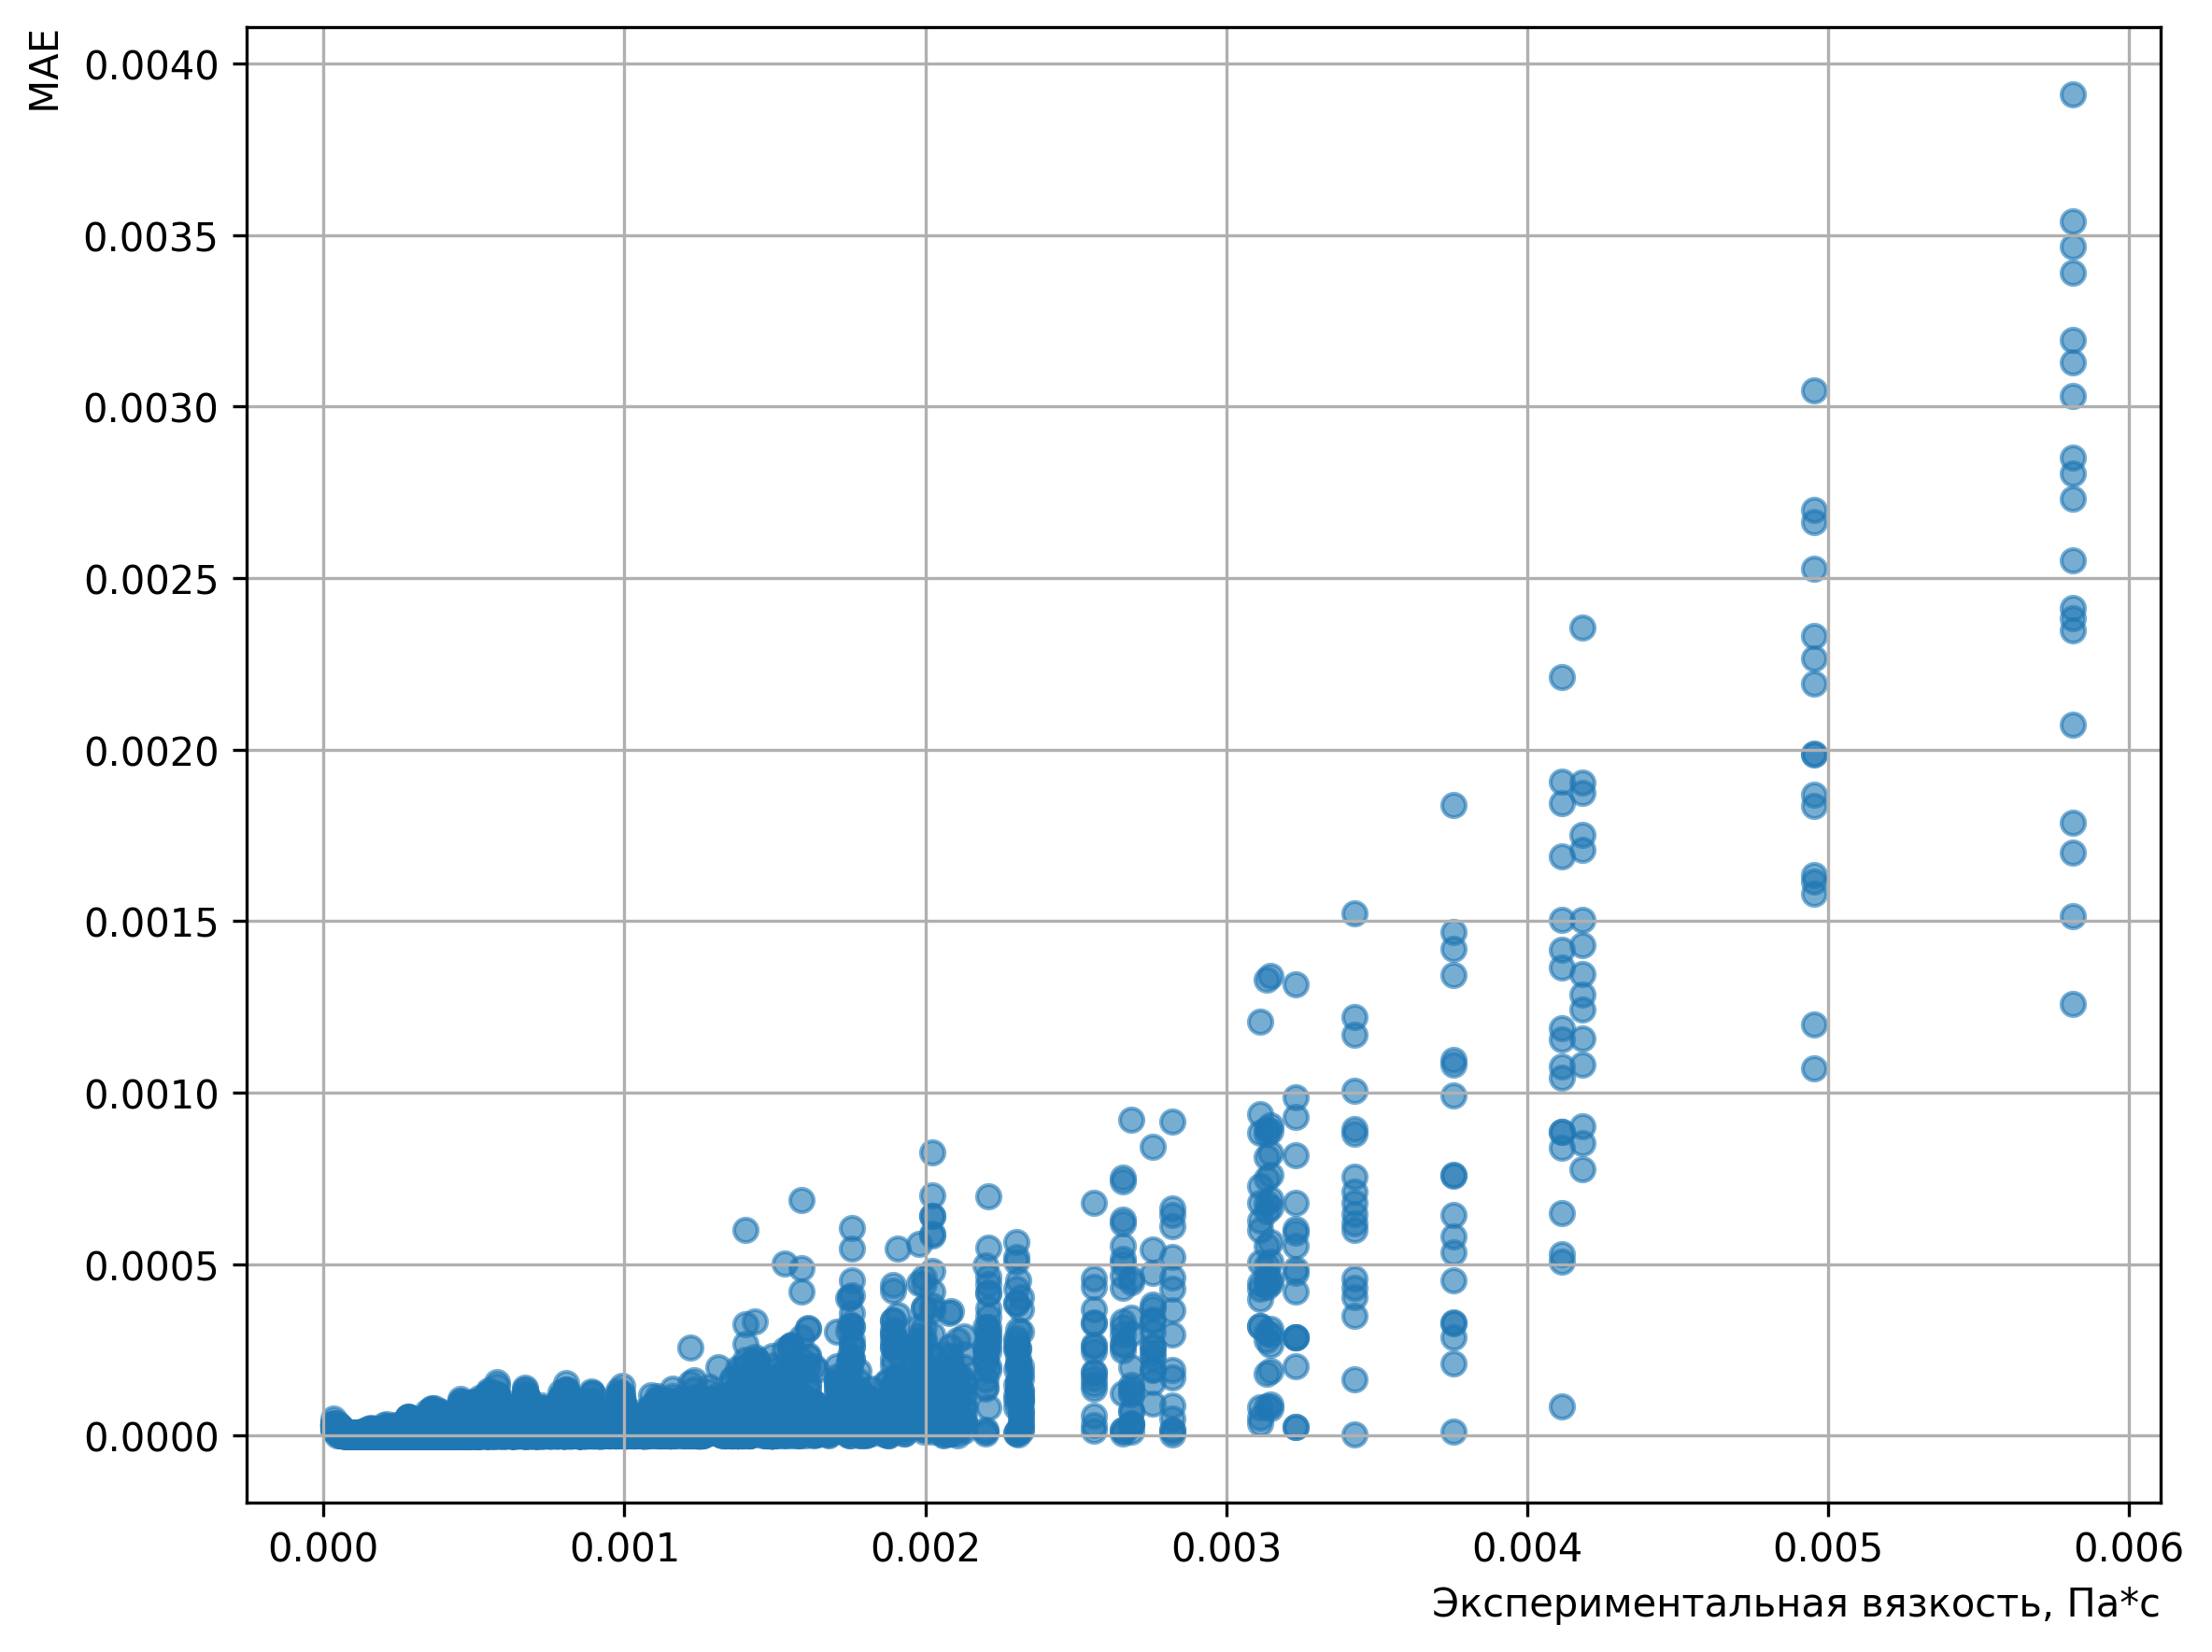
\includegraphics[width=\linewidth]{random_forest/MAE_Random Forest Model_0.8_rules.png}
          \caption{Абсолютная ошибка}
      \end{subfigure}
      \hfill
      \begin{subfigure}{0.48\textwidth}
          \centering
          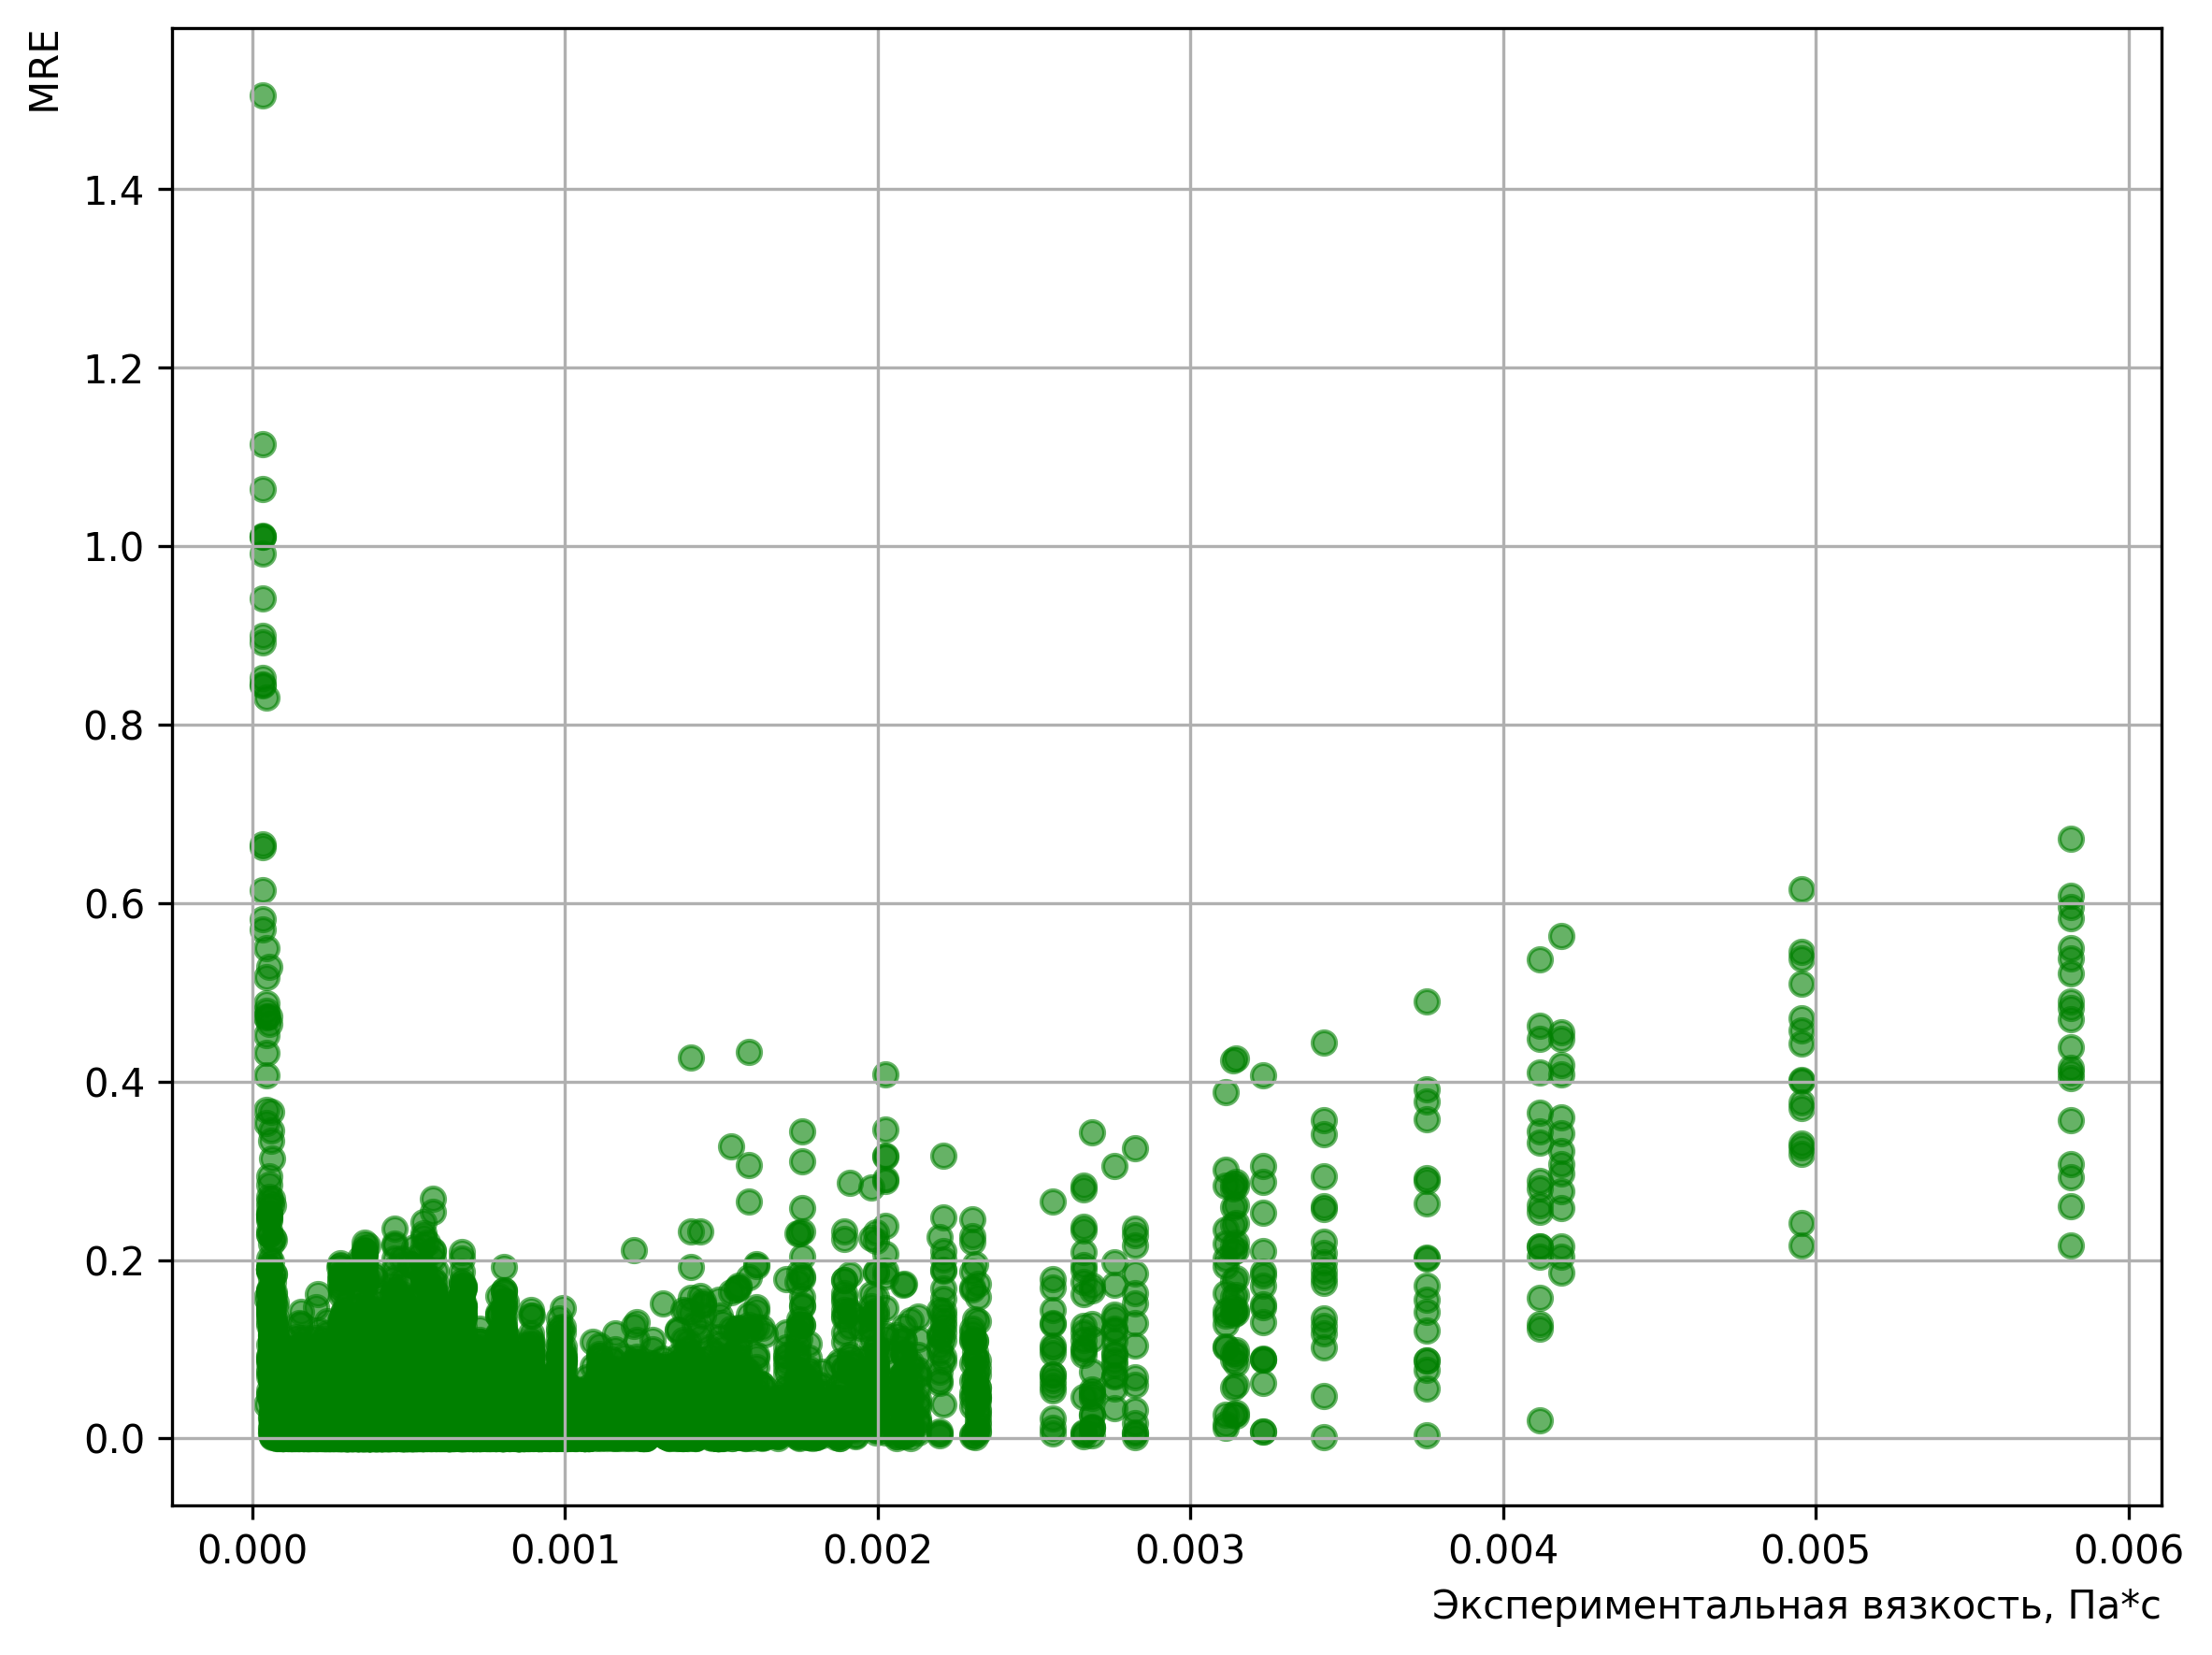
\includegraphics[width=\linewidth]{random_forest/MRE_Random Forest Model_0.8_rules.png}
          \caption{Относительная ошибка}
      \end{subfigure}
      \caption{Зависимость ошибки модели случайного леса от истинных значений вязкости. Расширенный набор признаков, малая обучающая выборка.}
      \label{fig:random_forest_errors_08_rules}
    \end{figure}
    
    \begin{minipage}{\textwidth}
      \textbf{Метрики качества (расширенные признаки, обучающая выборка 20\%):}
      \begin{itemize}
          \item RMSE: \( 1.10 \times 10^{-4} \) Па·с;
          \item MAE: \( 2.26 \times 10^{-5} \) Па·с;
          \item MRE: \( 0.0282 \).
      \end{itemize}
    \end{minipage}
    
    \subsubsection{Вывод по методу случайного леса}
    
    Модель случайного леса показала высокую точность и хорошую устойчивость к переобучению. Даже при сокращении обучающей выборки в четыре раза, она сохранила приемлемый уровень ошибок, что делает её надёжным инструментом для регрессии в условиях ограниченных данных. Использование расширенных признаков дополнительно повысило точность, особенно по метрике MAE. Как и в случае с методом ближайших соседей, RMSE оказался сравнительно выше, что свидетельствует о наличии отдельных точек с крупной ошибкой предсказания. Однако общее поведение модели позволяет считать случайный лес одной из самых надёжных и интерпретируемых моделей в рамках данного исследования.

  \subsection{Линейная регрессия}

    Линейная регрессия является одной из наиболее простых и интерпретируемых моделей машинного обучения. Её основное преимущество заключается в прозрачной структуре: каждое значение признака вносит линейный вклад в итоговое предсказание, а коэффициенты модели легко интерпретируются как меры влияния соответствующих признаков.

    В данной работе использовалась реализация \texttt{Ridge} из библиотеки \texttt{sklearn.linear\_model}. Модель c параметром регуляризации \( alpha = 0.003 \) показала наибольшую устойчивость. Остальные параметры остались без изменений. Перед использованием модели входные данные проходили нормализацию.
    
    \subsubsection{Оценка точности на большом обучающем наборе}
    
    При обучении модели на 80\% данных и использовании только базовых признаков линейная модель показала очень слабый результат. Оба предыдущих метода значительно превзошли линейную регрессию в данном случае. Результаты представлены на рисунке~\autoref{fig:linear_regression_errors_02_base}.
    
    \begin{figure}[ht!]
      \centering
      \begin{subfigure}{0.48\textwidth}
          \centering
          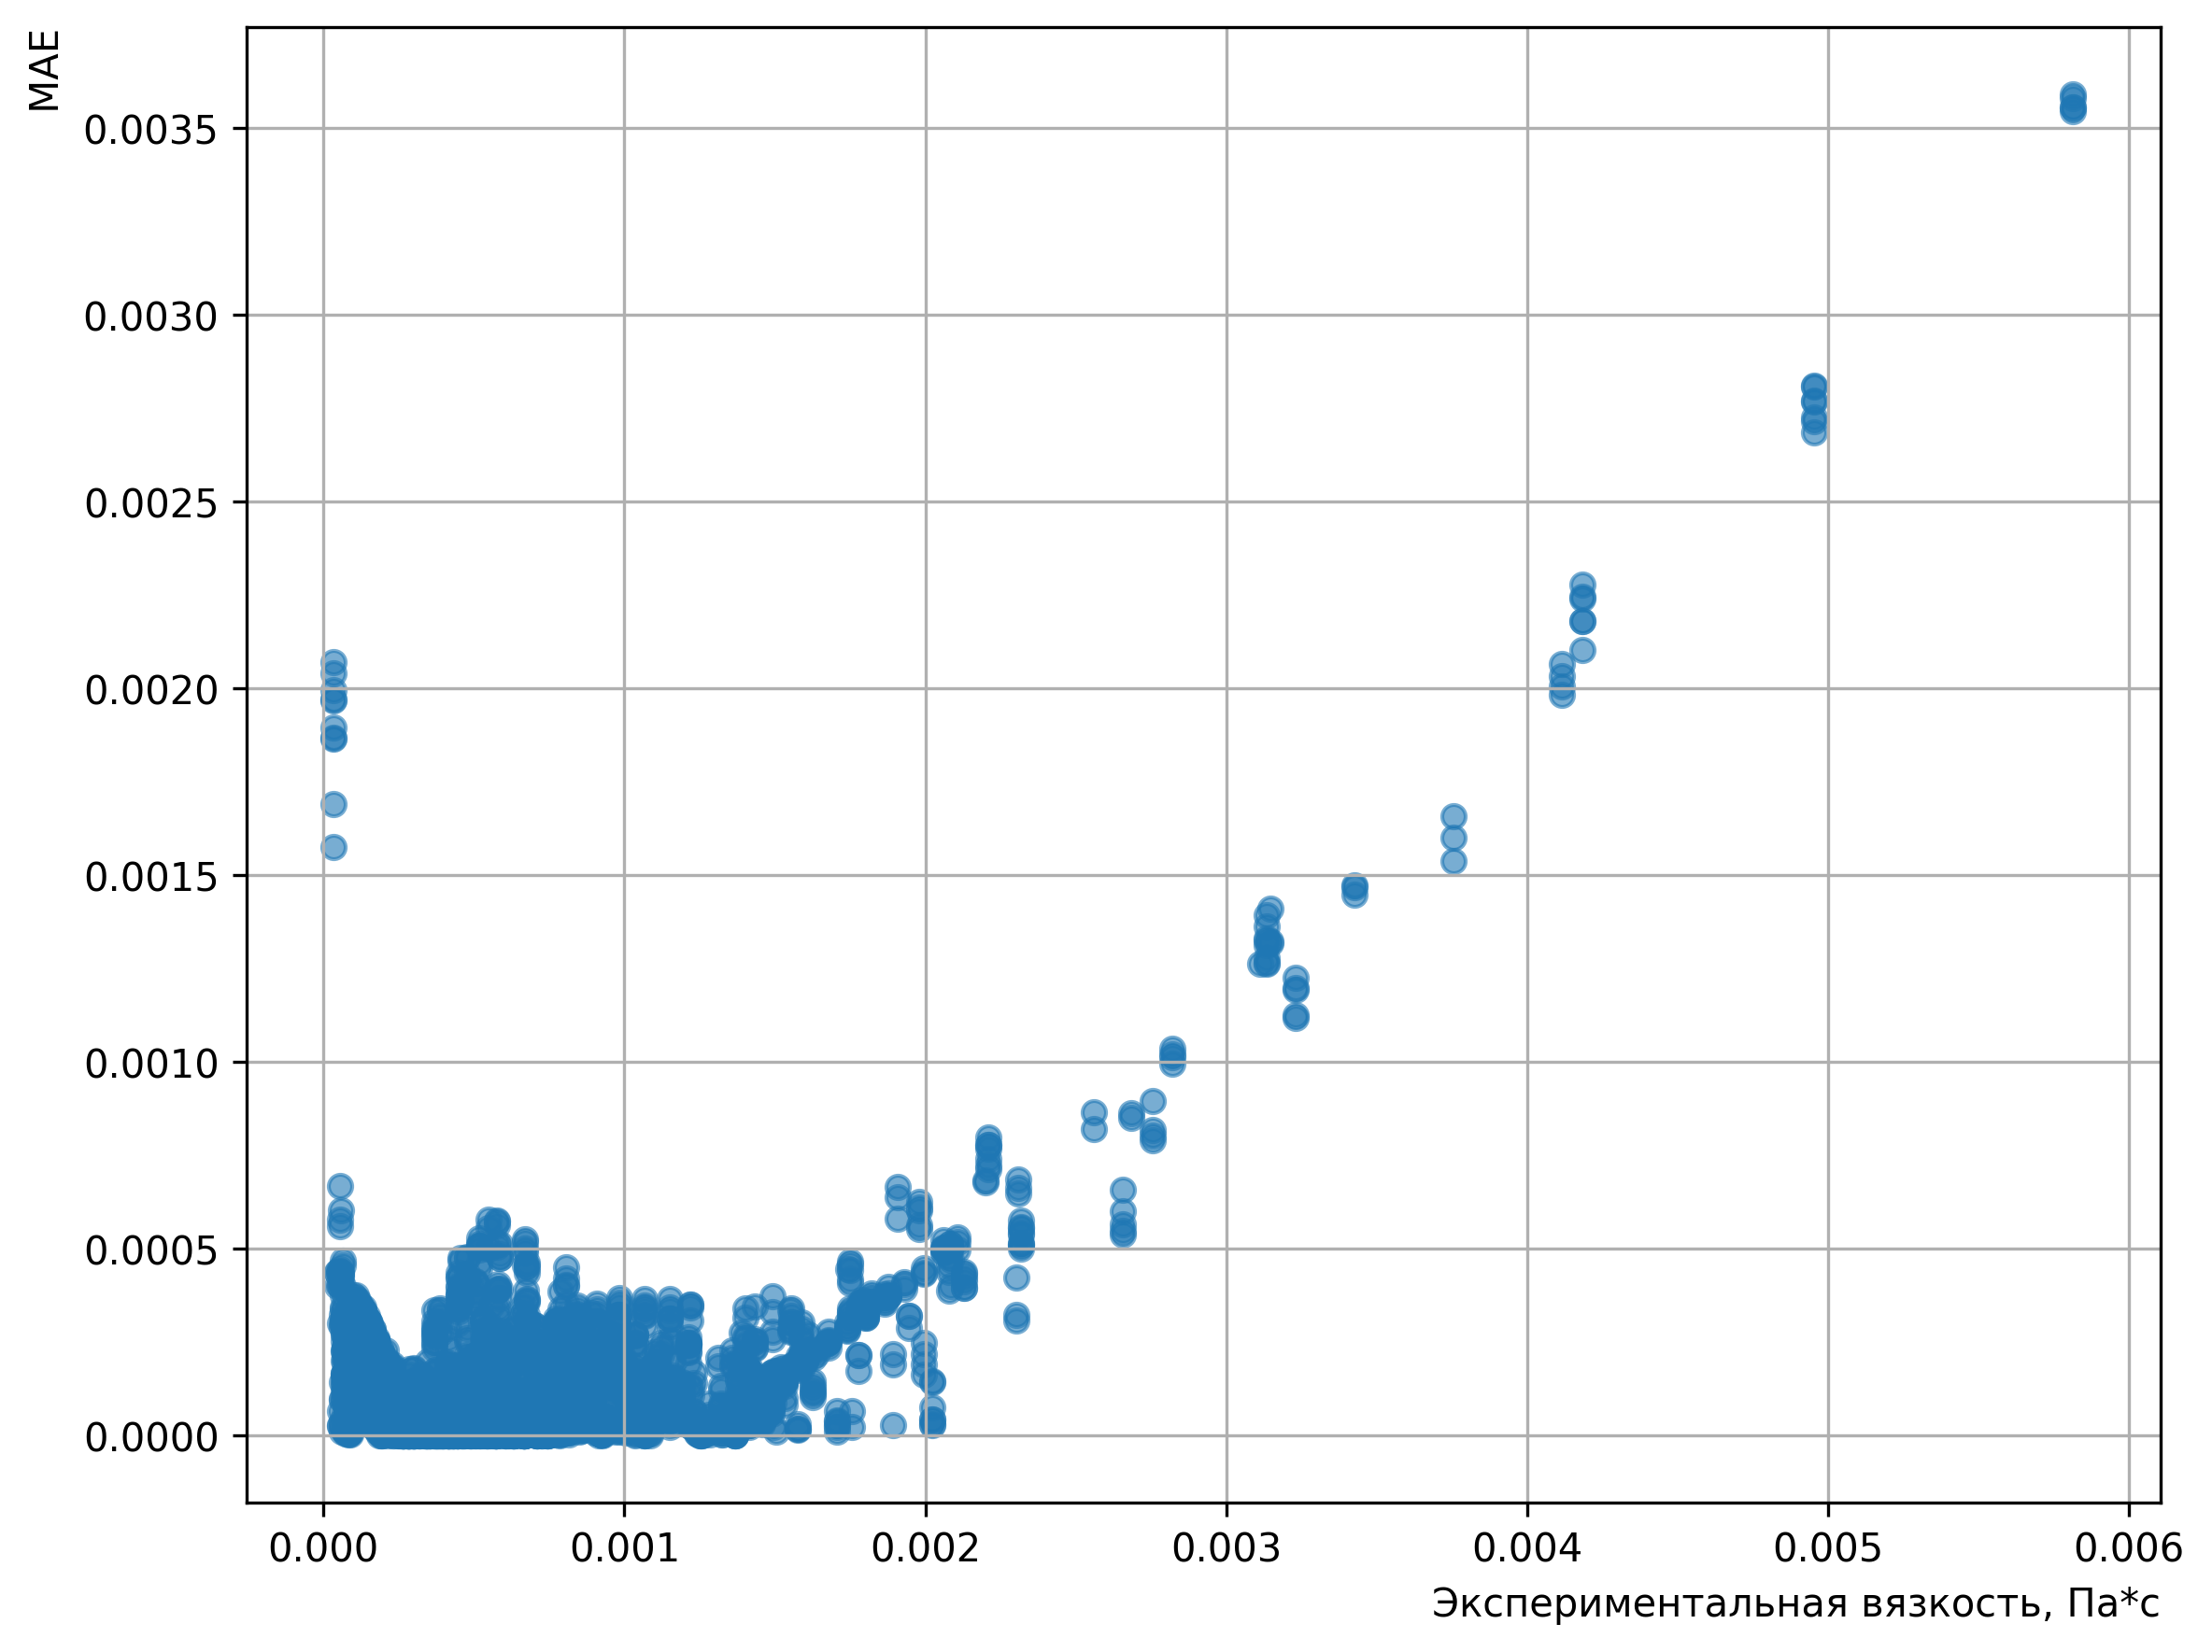
\includegraphics[width=\linewidth]{linear_regression/MAE_Linear Model_0.2_base.png}
          \caption{Абсолютная ошибка}
      \end{subfigure}
      \hfill
      \begin{subfigure}{0.48\textwidth}
          \centering
          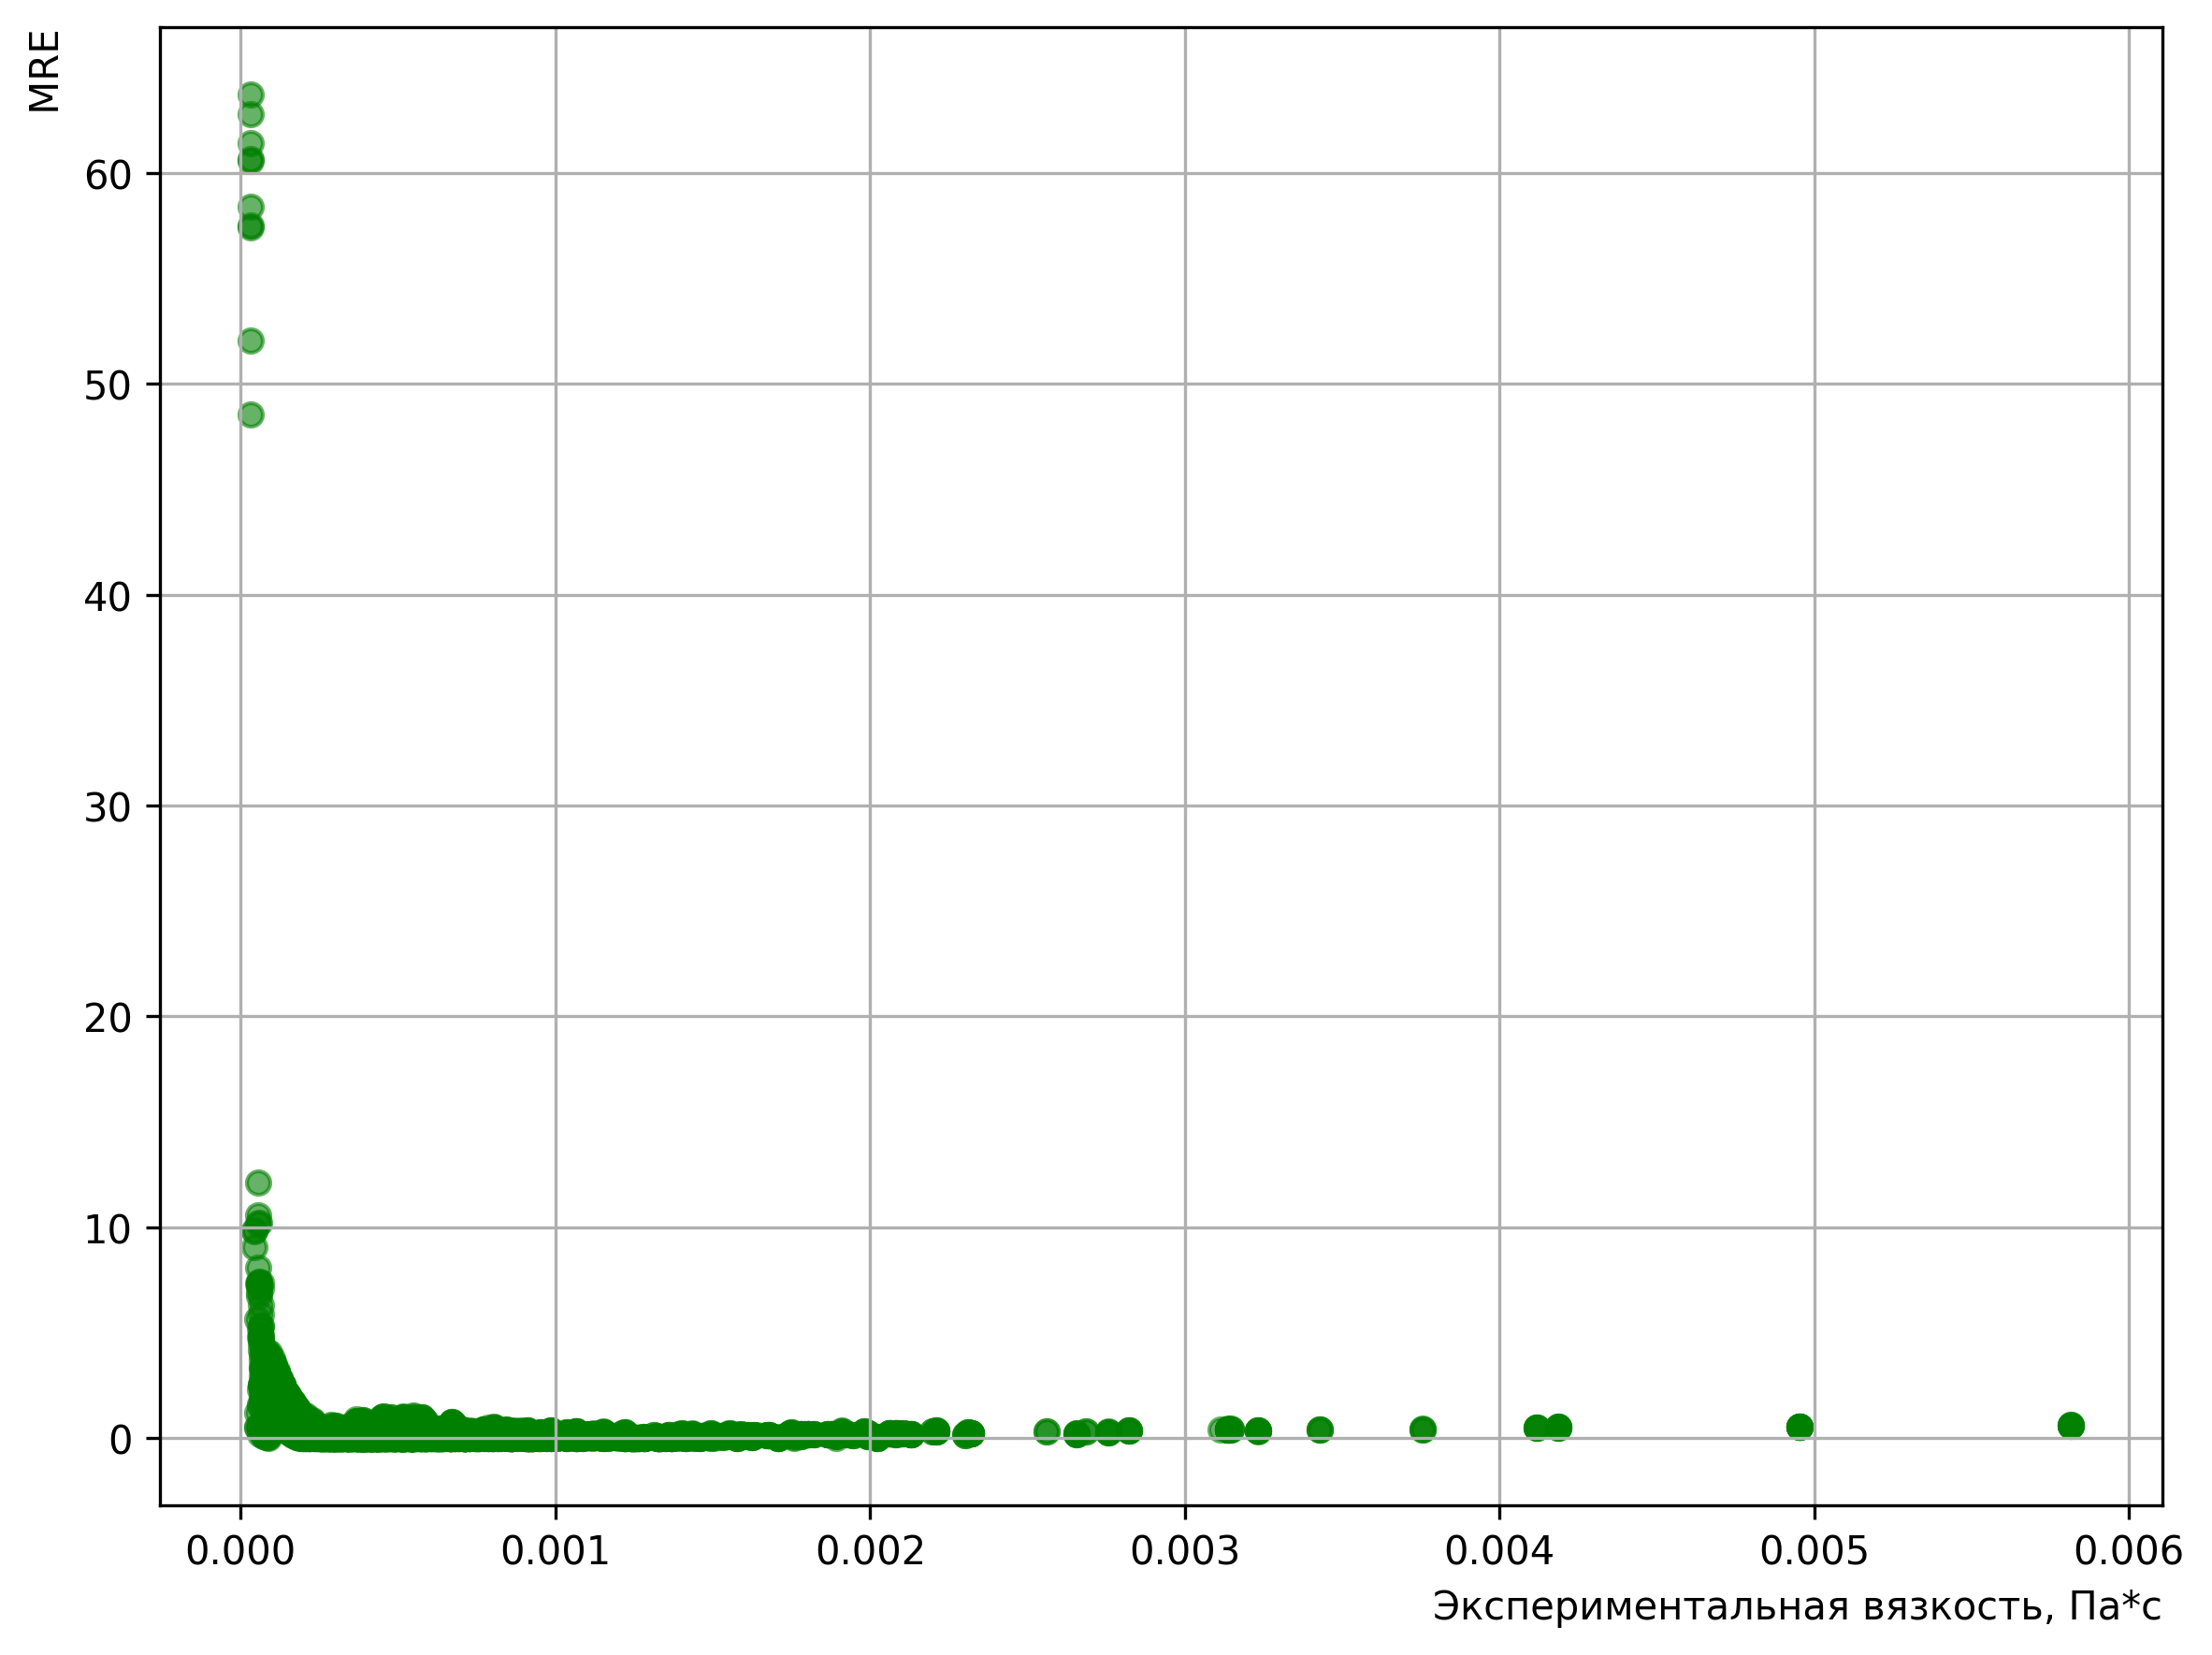
\includegraphics[width=\linewidth]{linear_regression/MRE_Linear Model_0.2_base.png}
          \caption{Относительная ошибка}
      \end{subfigure}
      \caption{Зависимость ошибки линейной регрессии от истинных значений вязкости. Базовый набор признаков, большая обучающая выборка.}
      \label{fig:linear_regression_errors_02_base}
    \end{figure}
    
    \begin{minipage}{\textwidth}
      \textbf{Метрики качества (базовые признаки, обучающая выборка 80\%):}
      \begin{itemize}
          \item RMSE: \( 2.35 \times 10^{-4} \) Па·с;
          \item MAE: \( 1.11 \times 10^{-4} \) Па·с;
          \item MRE: \( 0.3885 \).
      \end{itemize}
    \end{minipage}
    
    \subsubsection{Оценка на ограниченных данных}
    
    При обучении на 20\% данных модель не стала хуже, сохранив значения всех ошибок примерно на том же уровне. Это может говорить о том, что модель ограничена количеством признаков, а не количеством точек. Небольшую разницу в поведении модели можно увидеть на \autoref{fig:linear_regression_errors_08_base}.
    
    \begin{figure}[ht!]
      \centering
      \begin{subfigure}{0.48\textwidth}
          \centering
          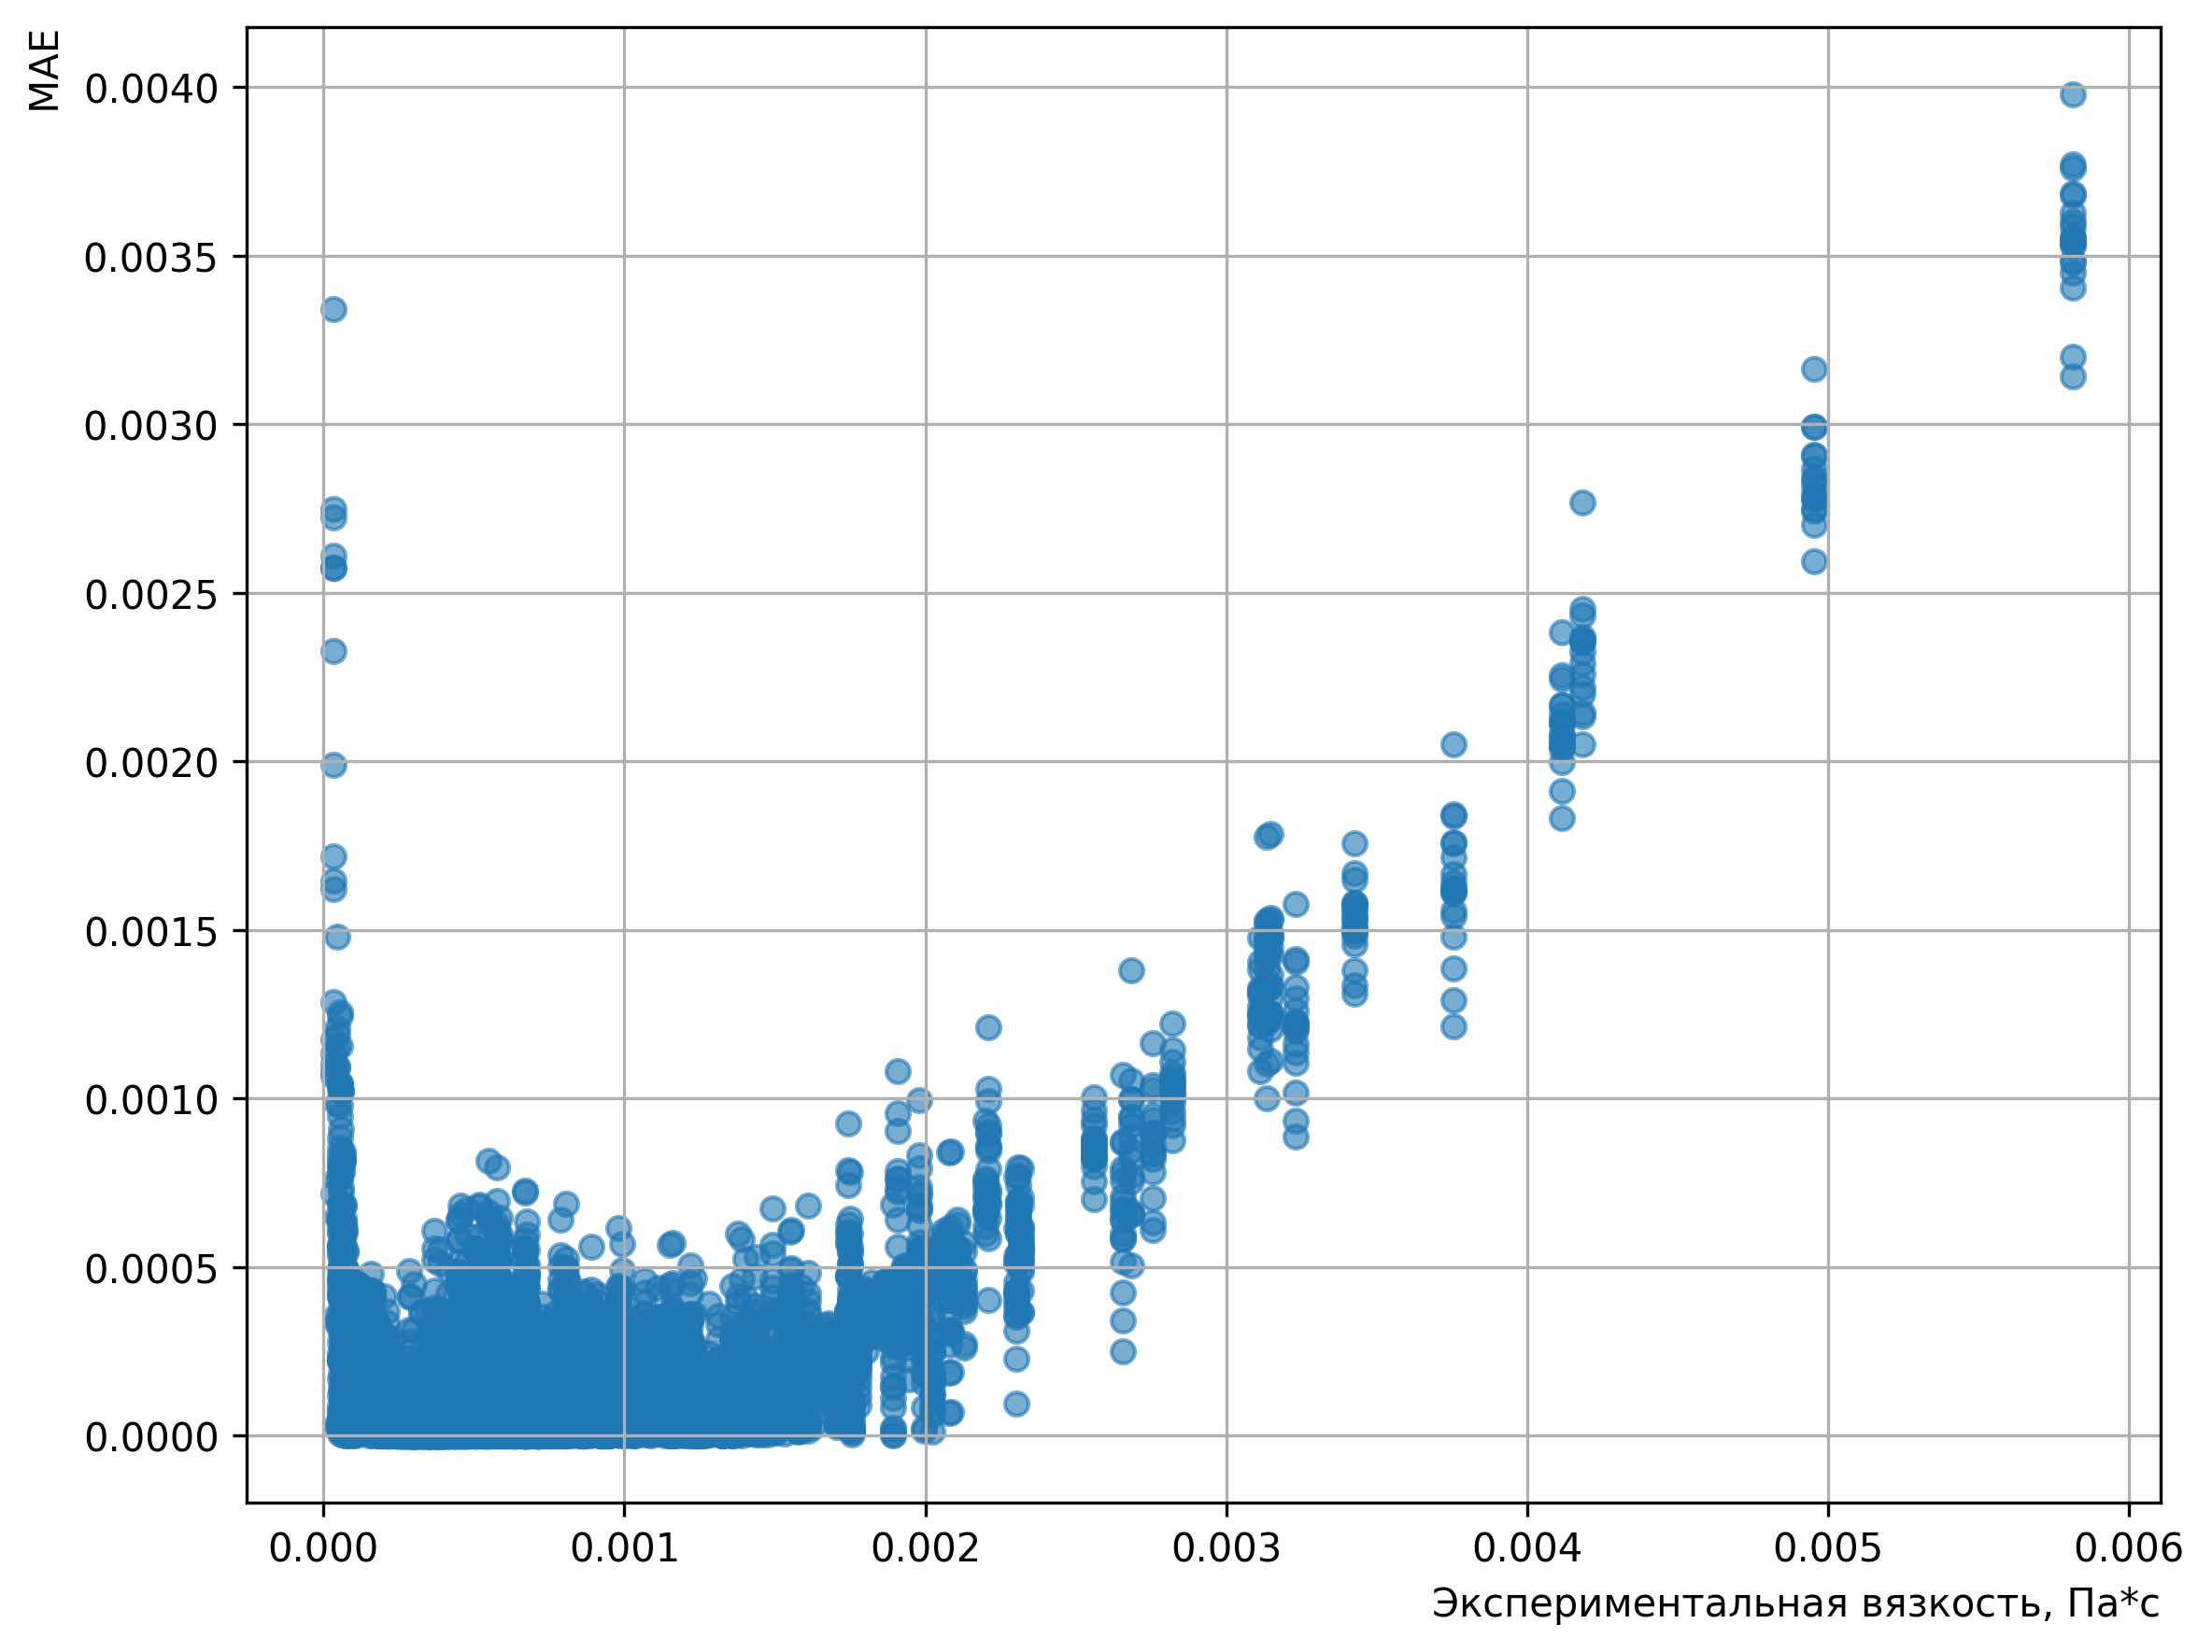
\includegraphics[width=\linewidth]{linear_regression/MAE_Linear Model_0.8_base.png}
          \caption{Абсолютная ошибка}
      \end{subfigure}
      \hfill
      \begin{subfigure}{0.48\textwidth}
          \centering
          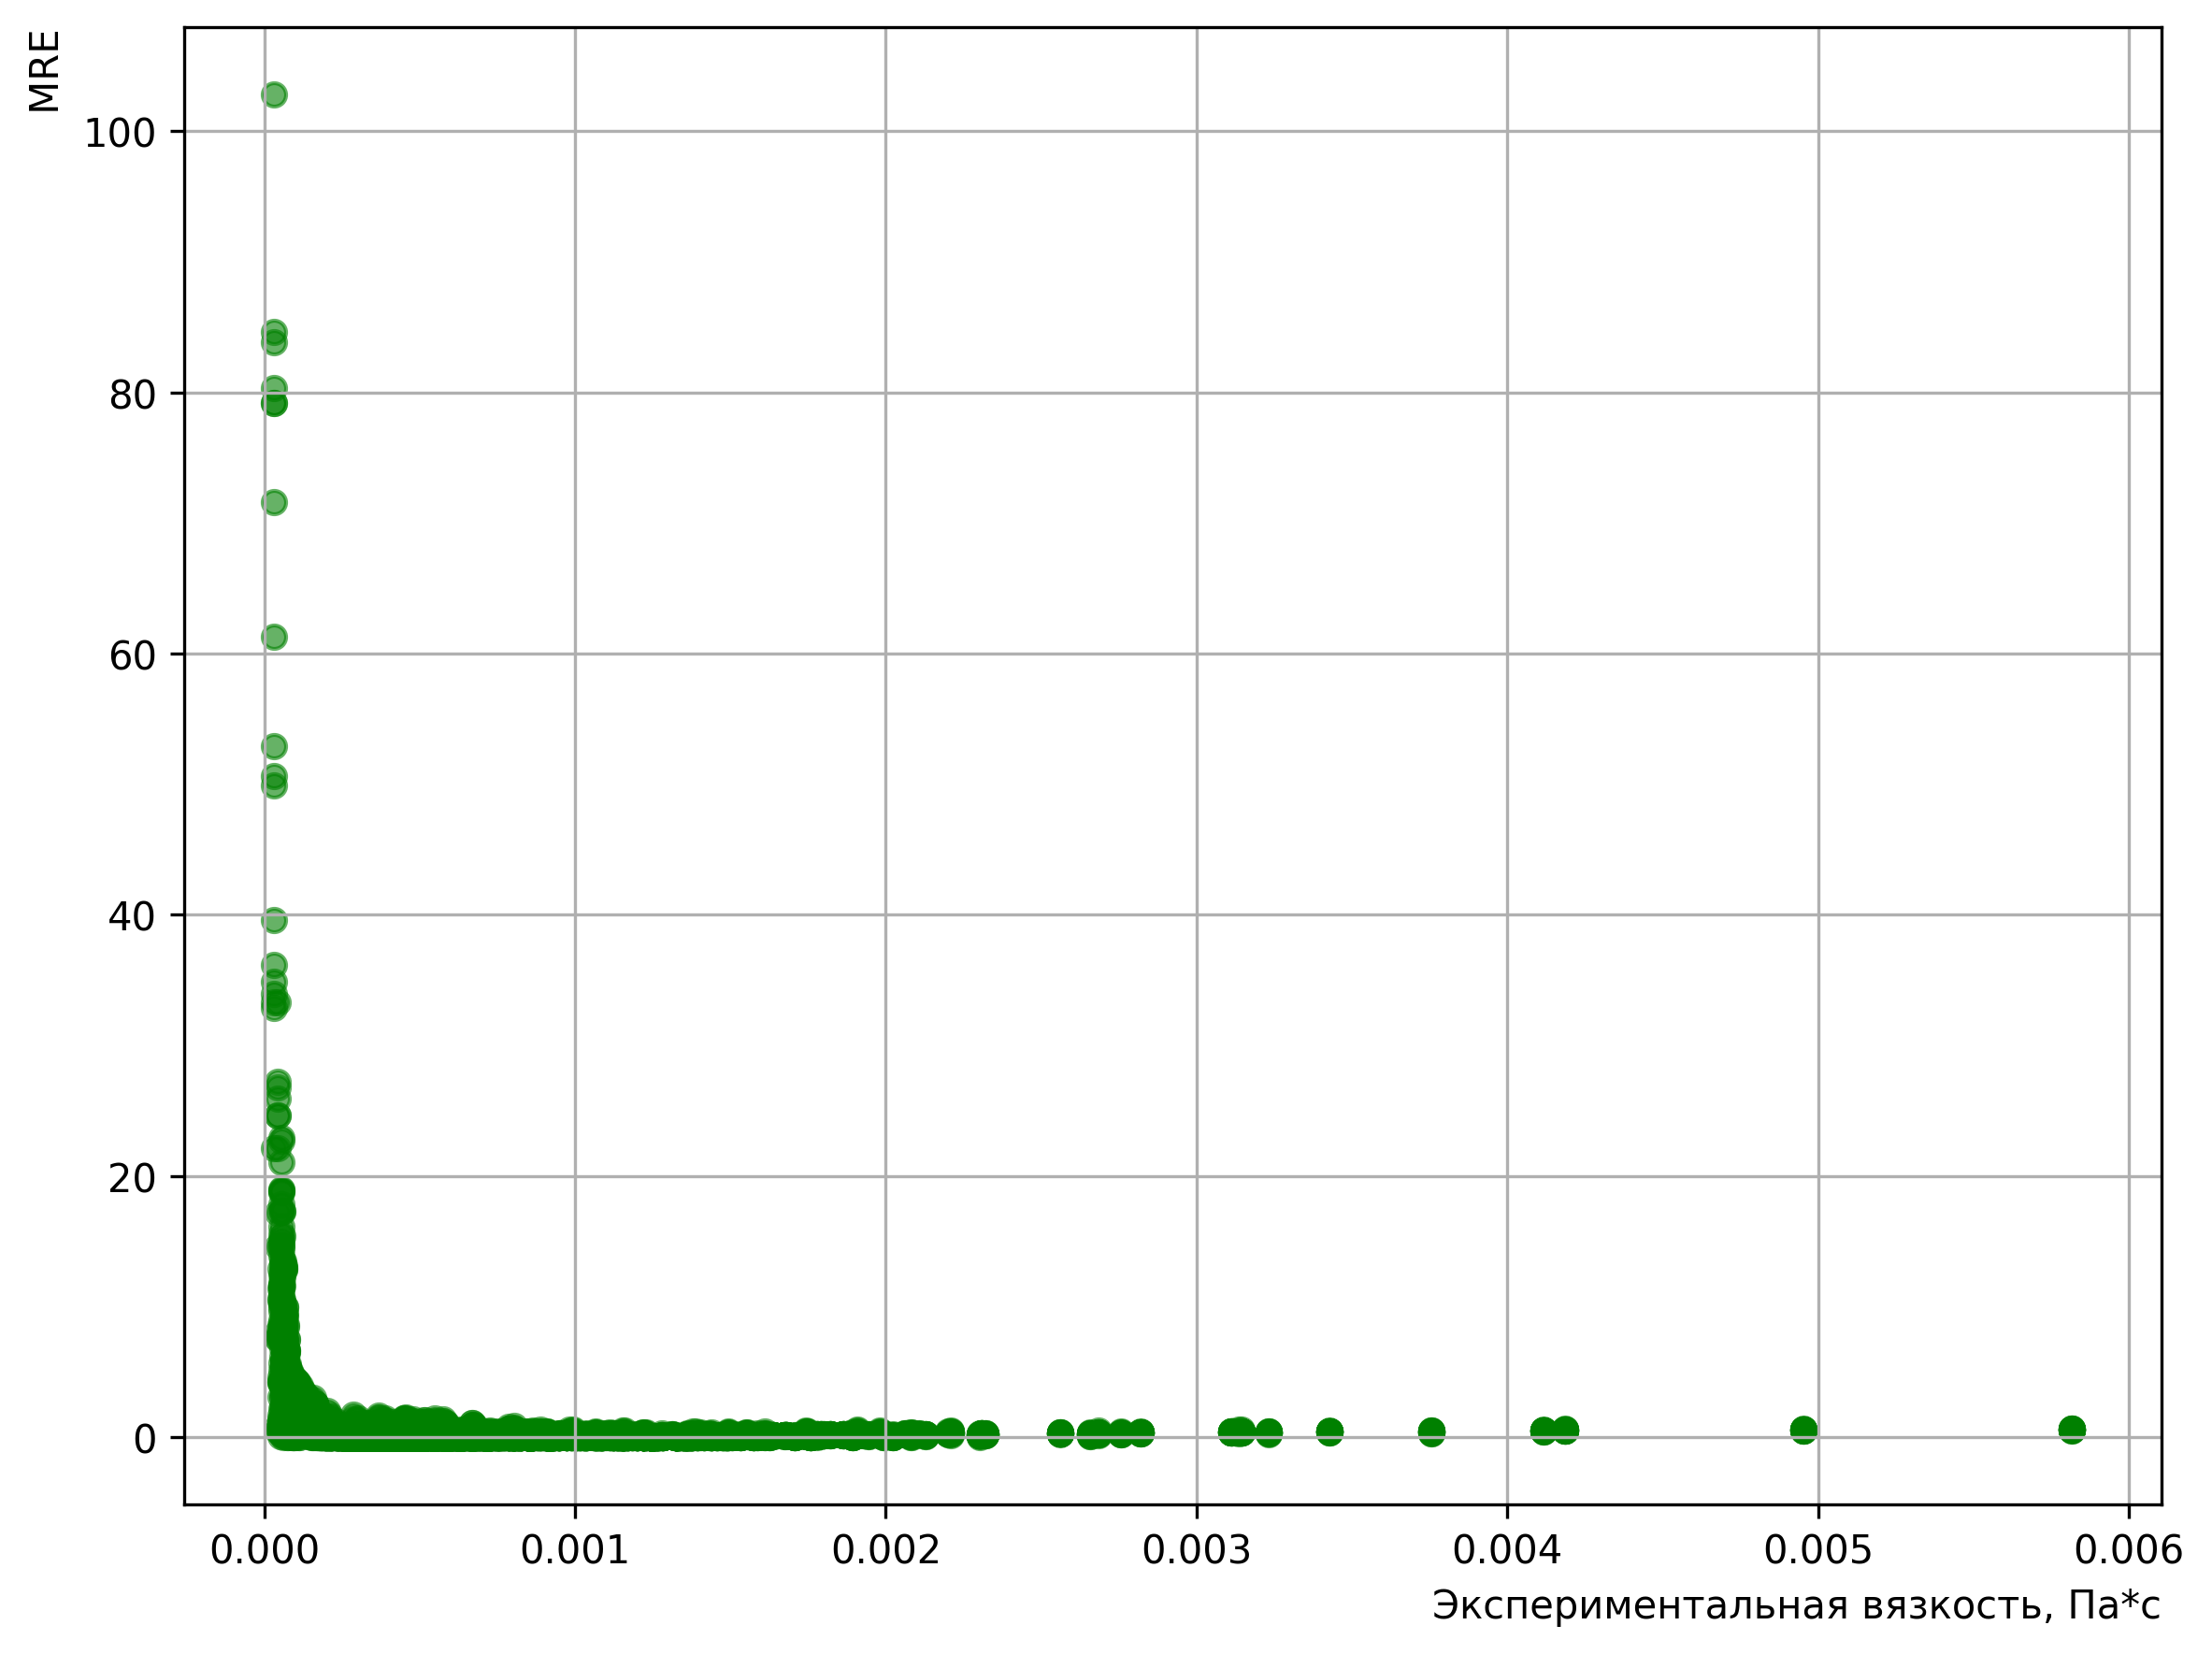
\includegraphics[width=\linewidth]{linear_regression/MRE_Linear Model_0.8_base.png}
          \caption{Относительная ошибка}
      \end{subfigure}
      \caption{Зависимость ошибки линейной регрессии от истинных значений вязкости. Базовый набор признаков, малая обучающая выборка.}
      \label{fig:linear_regression_errors_08_base}
    \end{figure}
    
    \begin{minipage}{\textwidth}
    \textbf{Метрики качества (базовые признаки, обучающая выборка 20\%):}
      \begin{itemize}
          \item RMSE: \( 2.29 \times 10^{-4} \) Па·с;
          \item MAE: \( 1.08 \times 10^{-4} \) Па·с;
          \item MRE: \( 0.3628 \).
      \end{itemize}
    \end{minipage}
    
    \subsubsection{Влияние расширенных признаков}
    
    При использовании расширенных признаков и обучении на 20\% выборки результаты стали гораздо лучше. Модель значительно превзошла корреляцию MYS по всем трем метрикам. При этом значение ошибки MRE выше, чем в методе случайного леса. Однако и здесь относительная ошибка менее 5\%, что позволяет заявить, что данный метод пригоден для прикладных задач. 

    На графиках, демонстрирующих метрики \autoref{fig:linear_regression_errors_08_rules} можно заметить много точек, дающих большую абсолютную ошибку, несмотря на маленькие значения истинной вязкости. Недолгий анализ выявил, что эти точки находятся вблизи критической точки. Большая часть из них имеют давление около 3 МПа и температуру от 400 градусов. На основании этого можно сделать вывод, что линейная регрессия может испытывать трудности при определении свойств смесей вблизи критической точки. 
    
    \begin{figure}[ht!]
      \centering
      \begin{subfigure}{0.48\textwidth}
          \centering
          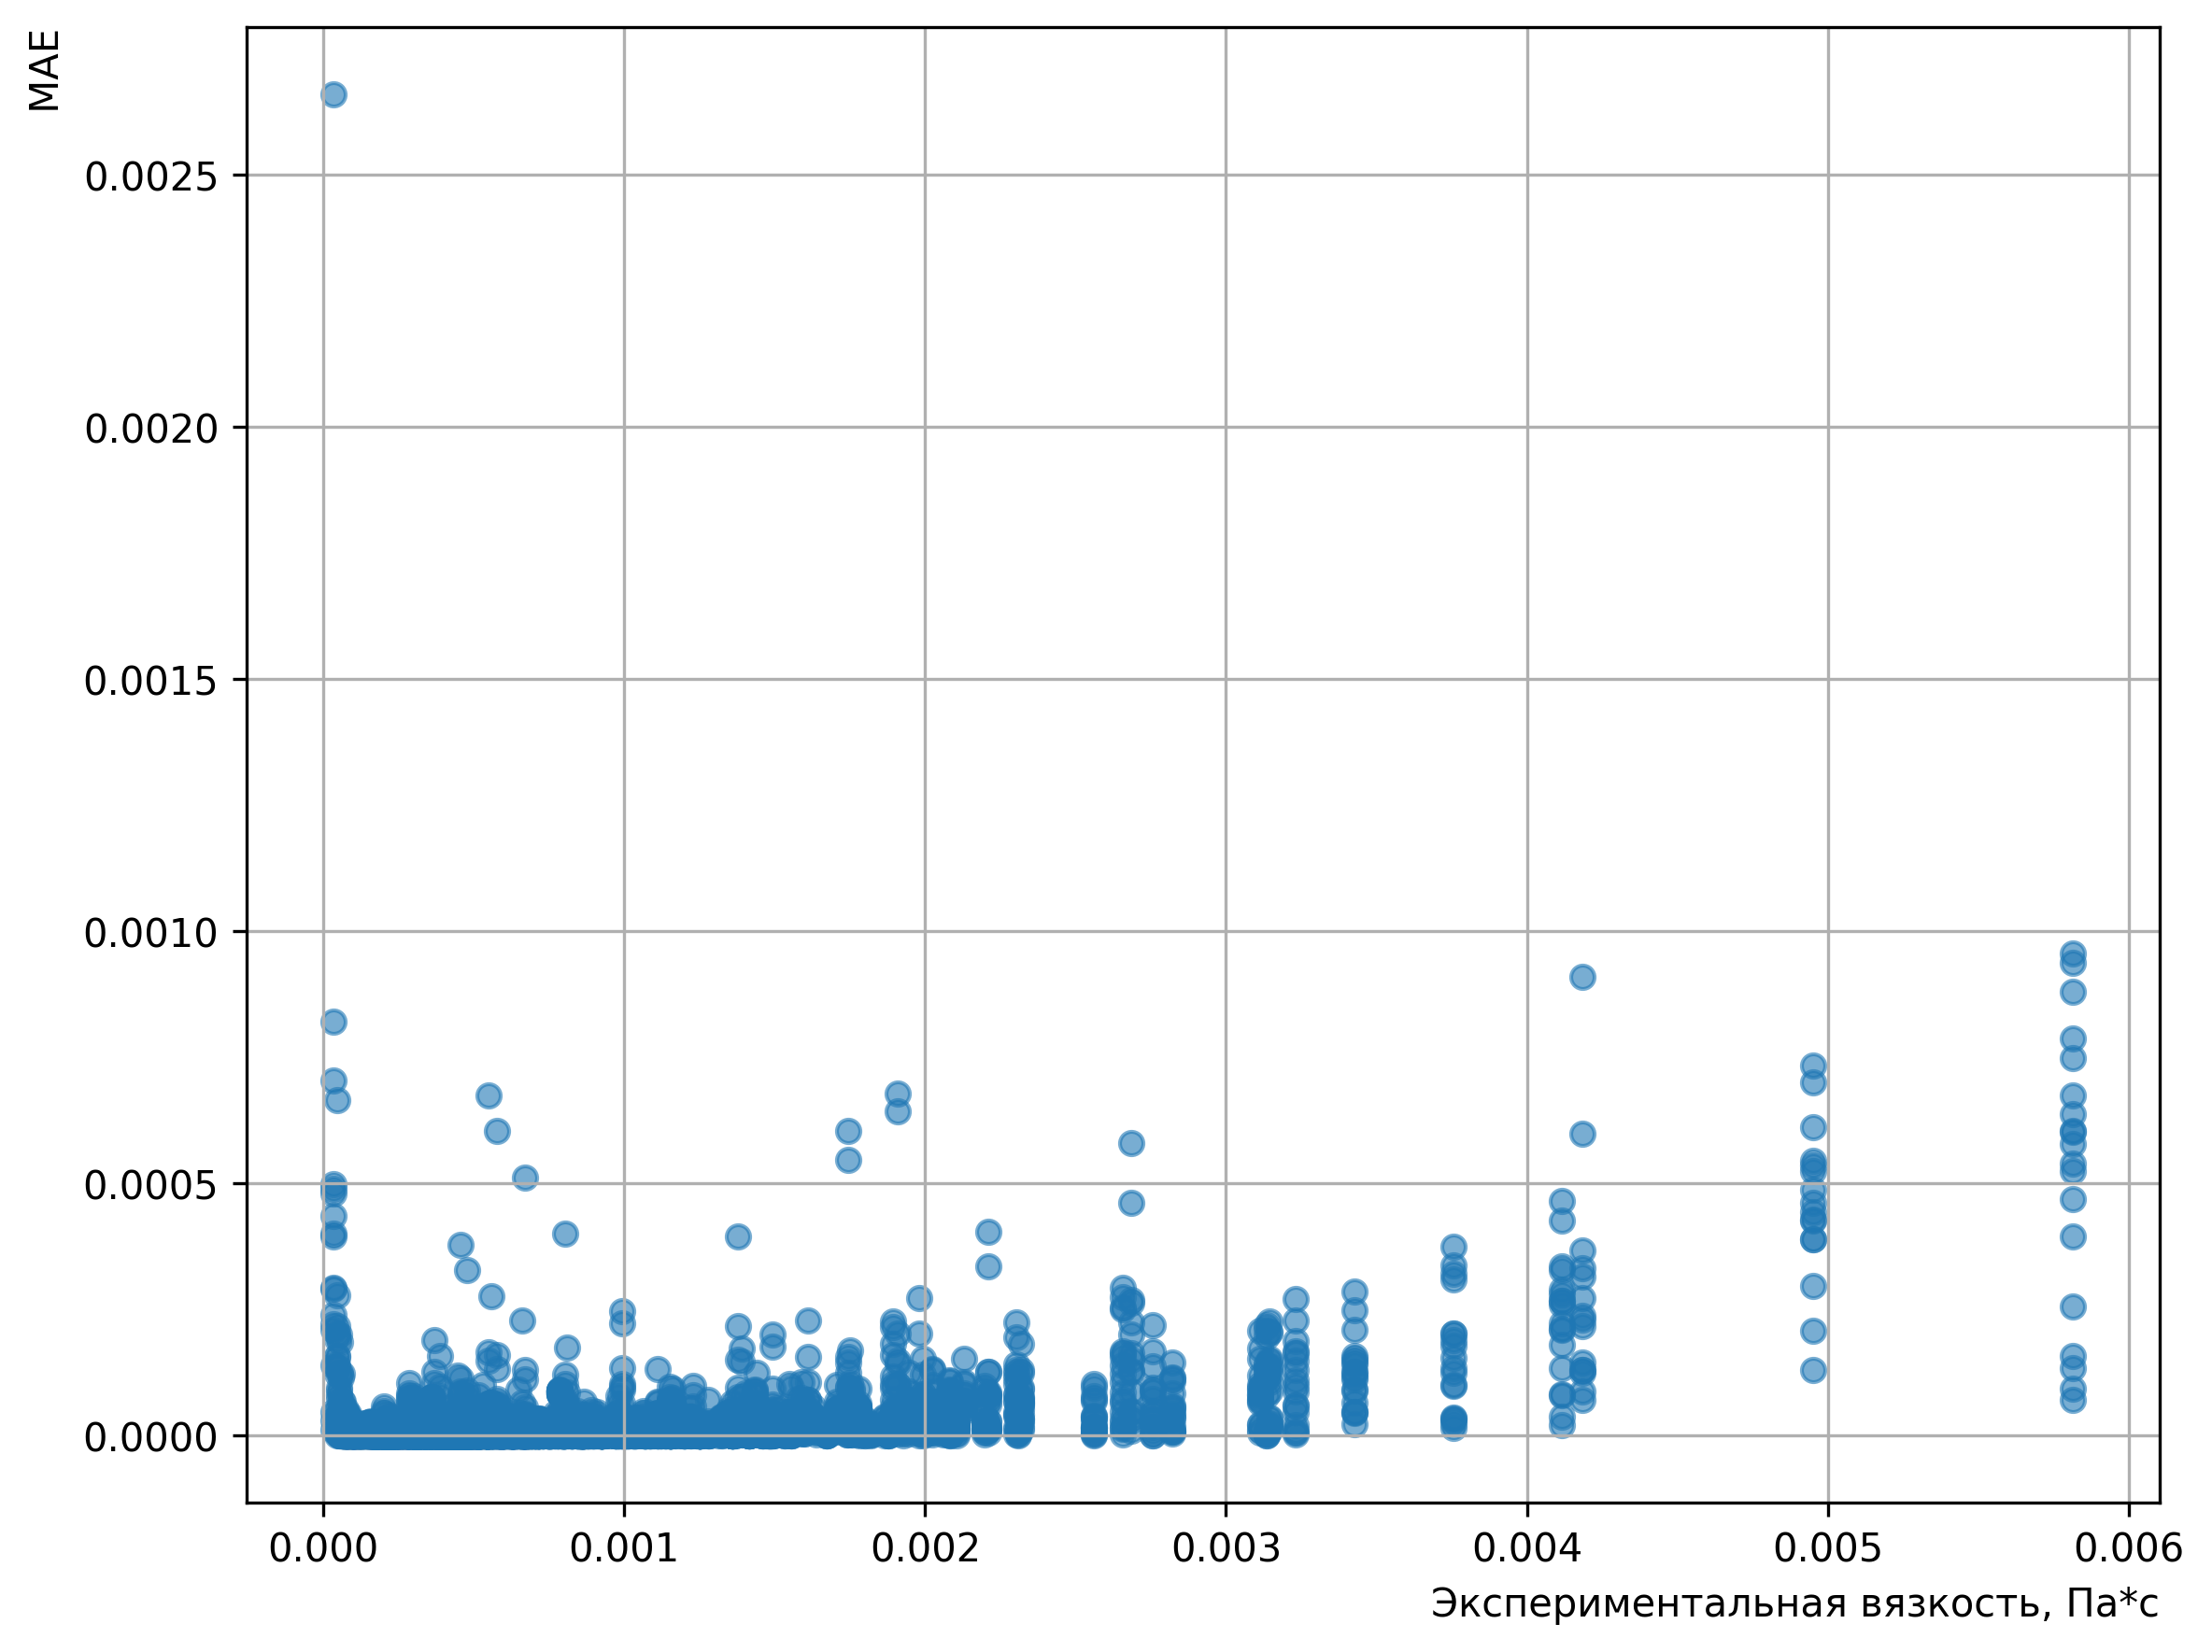
\includegraphics[width=\linewidth]{linear_regression/MAE_Linear Model_0.8_rules.png}
          \caption{Абсолютная ошибка}
      \end{subfigure}
      \hfill
      \begin{subfigure}{0.48\textwidth}
          \centering
          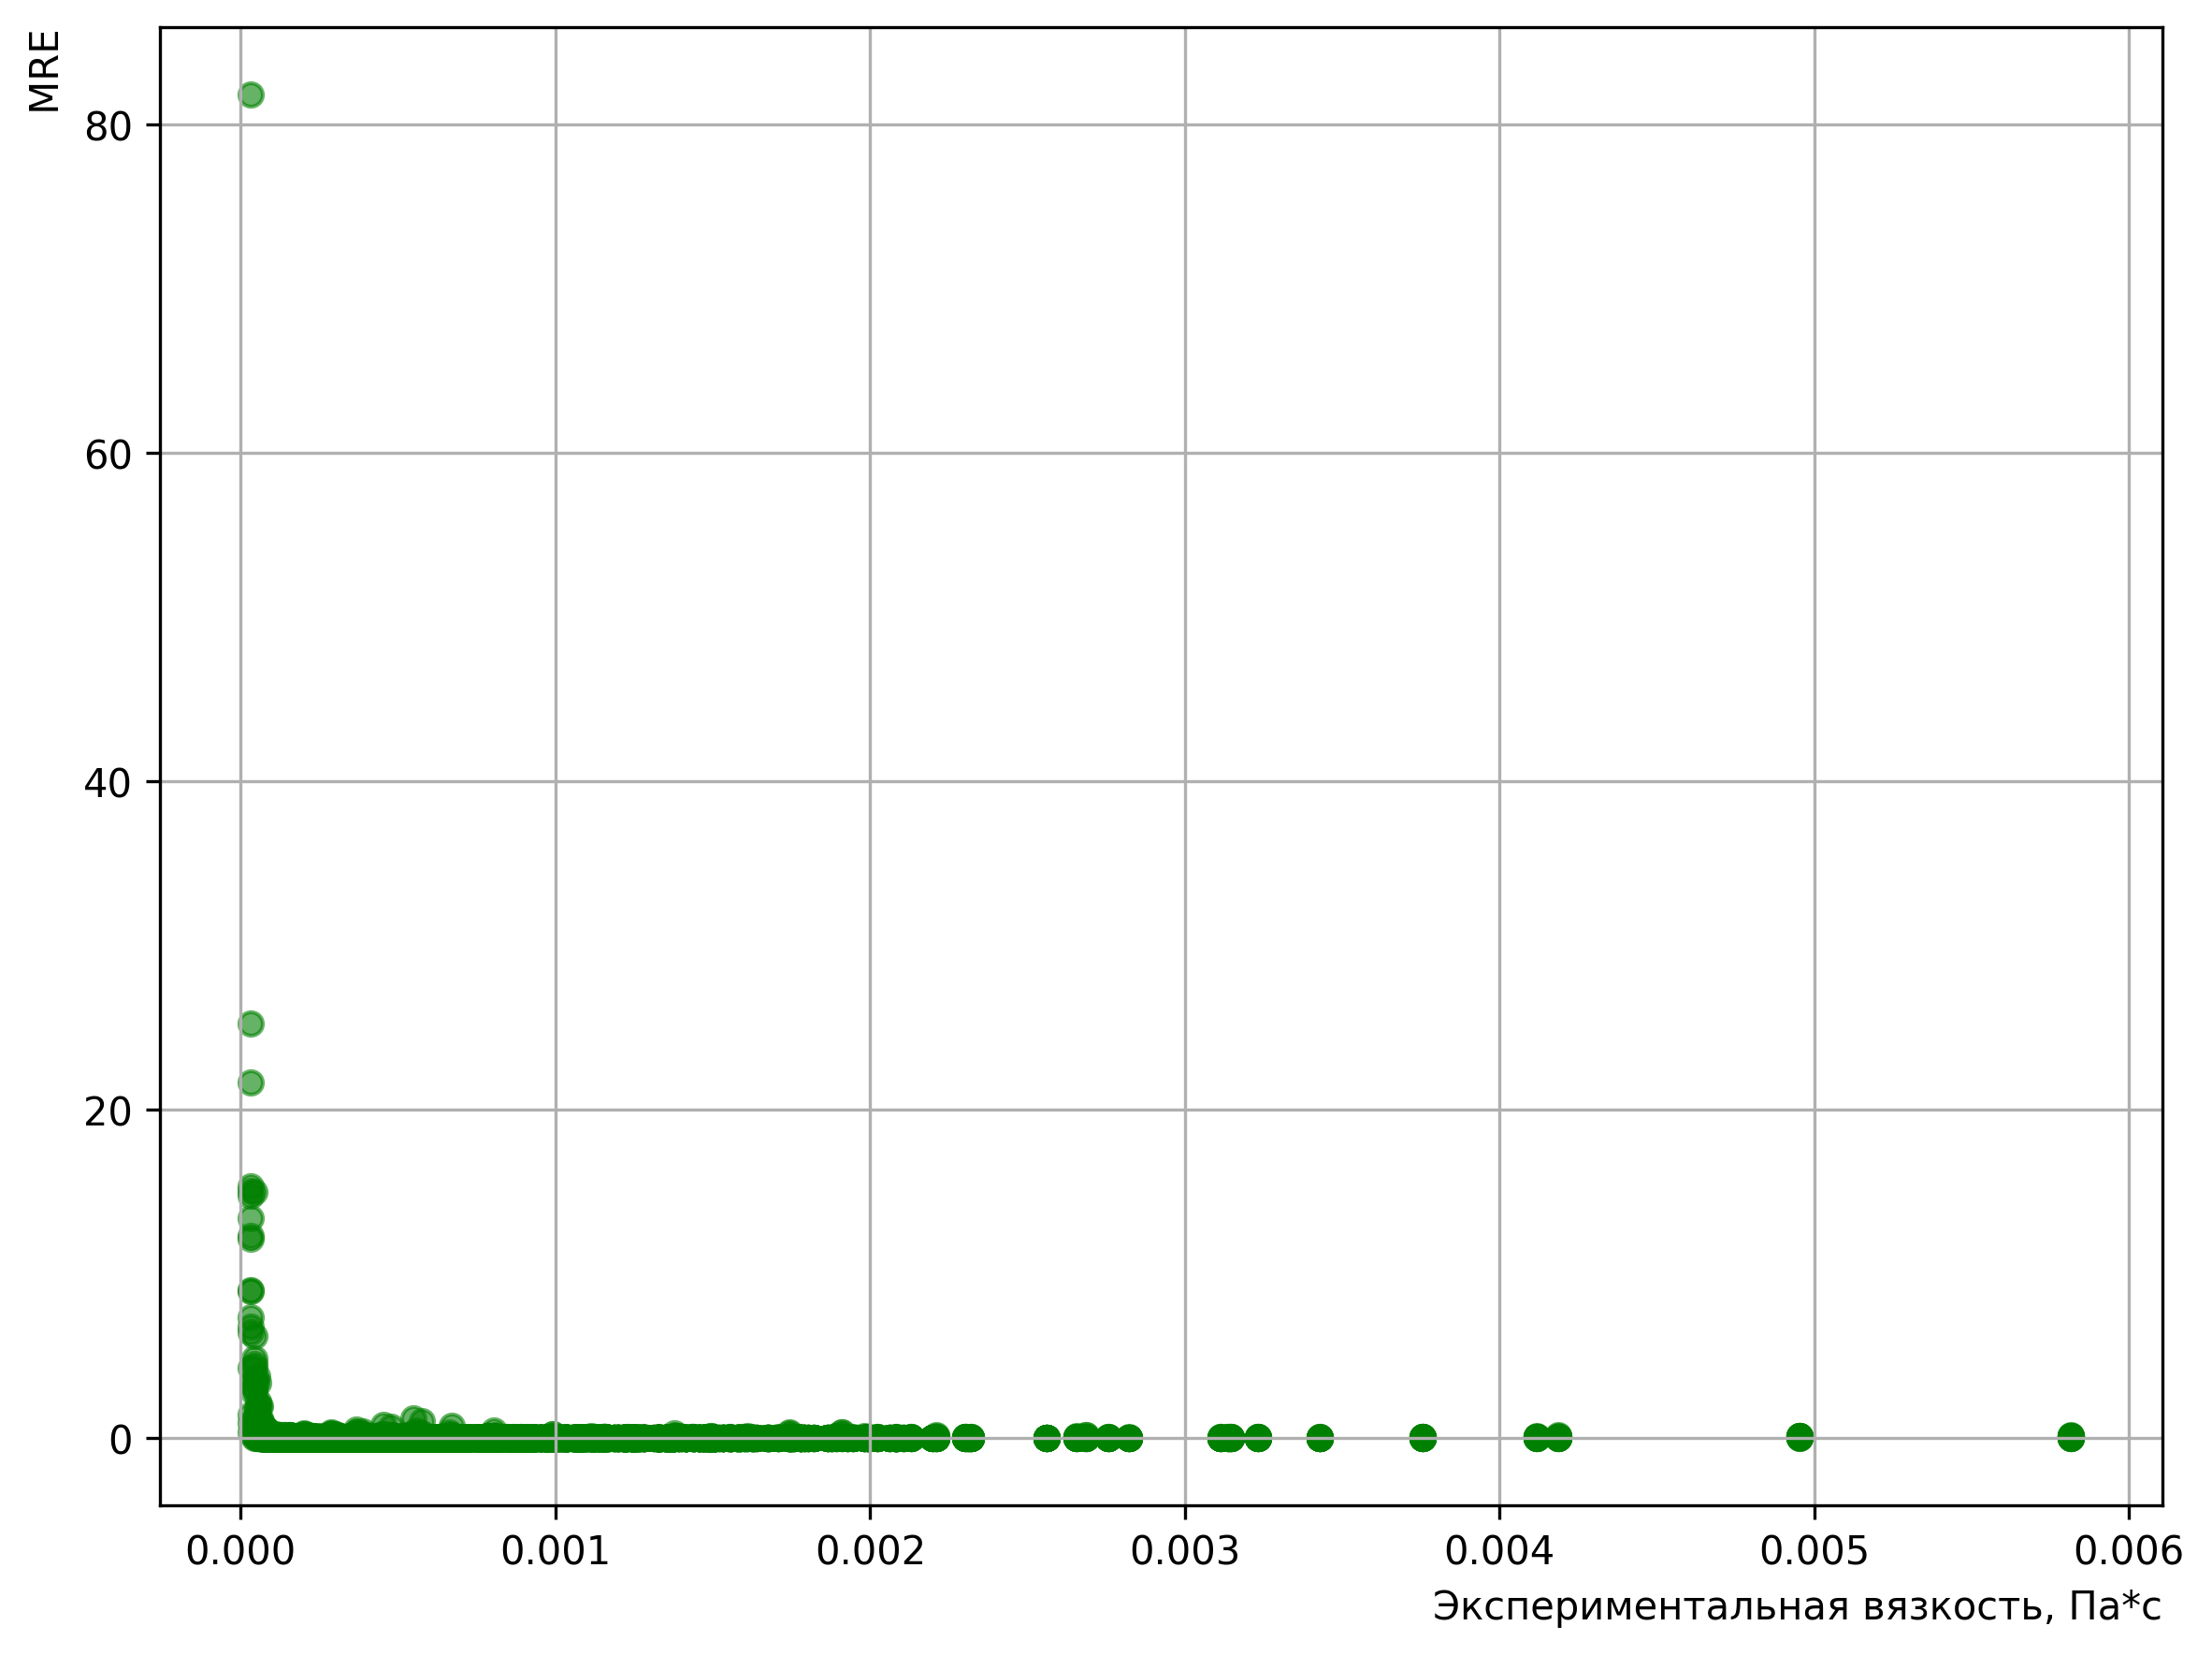
\includegraphics[width=\linewidth]{linear_regression/MRE_Linear Model_0.8_rules.png}
          \caption{Относительная ошибка}
      \end{subfigure}
      \caption{Зависимость ошибки линейной регрессии от истинных значений вязкости. Расширенный набор признаков, малая обучающая выборка.}
      \label{fig:linear_regression_errors_08_rules}
    \end{figure}
    
    \begin{minipage}{\textwidth}
      \textbf{Метрики качества (расширенные признаки, обучающая выборка 20\%):}
      \begin{itemize}
          \item RMSE: \( 3.39 \times 10^{-5} \) Па·с;
          \item MAE: \( 1.05 \times 10^{-5} \) Па·с;
          \item MRE: \( 0.0320 \).
      \end{itemize}
    \end{minipage}

    \subsubsection{Вывод по линейной регрессии}

      Линейная регрессия, как и ожидалось, показала ограниченные возможности на базовом наборе признаков. Наиболее ярко это проявилось в эксперименте с большой обучающей выборкой, где модель не смогла захватить сложные зависимости между параметрами, несмотря на большое количество данных. Это указывает скорее на фундаментальную слабость модели в предсказании признаков на основании малого числа входных параметров, чем на недостаточный размер обучающих данных. Интересным наблюдением стало и то, что уменьшение обучающей выборки практически не повлияло на качество линейной модели.

      На фоне этого особенно показательной стала роль расширенных признаков. Добавление сгенерированных признаков позволило резко улучшить точность предсказаний, особенно по метрикам RMSE и MAE. Это подтверждает предположение о том, что основной ограничивающий фактор линейной модели, это ее ограниченная гибкость -- точность в большей степени определялась признаками, а не объёмом данных.
      
      Отдельного внимания заслуживают зоны, в которых линейная модель особенно плохо справлялась с предсказанием -- вблизи критических точек. В частности, ошибки резко возрастали при давлениях около 3 МПа и температурах порядка 400 К. Скорее всего, это можно исправить, если генерировать признаки с упором на описание данных областей или если увеличить количество похожих данных.
      
      В результате, несмотря на простоту, линейная модель, обученная на расширенном признаковом пространстве, продемонстрировала наилучшие метрики среди всех протестированных подходов. Особенно важно, что средняя относительная ошибка не превышала 5\%, что делает подход пригодным для прикладного использования, в том числе в инженерных расчётах и быстрых приближённых оценках.

  \subsection{Сравнение подходов}

    В данном подразделе будет произведено сравнение моделей. Логичнее всего сравнить их, обучая на малых данных, так как это позволяет оценить способность к обобщению, а также дает адекватное преимущество уравнению MYS. Также, использовались расширенные данные, потому что на них у всех моделей точность выше.  

  \begin{table}[ht!]
    \TableNumberRight
    \begin{center}
      \textbf{Характеристики ошибок для различных моделей}
      \vspace*{\fill}
    \end{center}
    
    \vspace{0.8ex}
    \noindent

    \begin{tabular}{|l|c|c|c|}
        \hline
        \textbf{Модель} & \textbf{RMSE} (\(\times 10^{-4}\) Па·с) & \textbf{MAE} (\(\times 10^{-5}\) Па·с) & \textbf{MRE} \\
        \hline
        KNN & \( 1.62 \pm 0.33 \) & \( 4.65 \pm 0.53 \) & \( 0.0594 \pm 0.0044 \) \\
        Случайный лес & \( 1.10 \pm 0.35 \) & \( 2.24 \pm 0.46 \) & \( 0.0280 \pm 0.0027 \) \\
        Линейная регрессия & \( 0.34 \pm 0.14 \) & \( 1.05 \pm 0.14 \) & \( 0.0320 \pm 0.0173 \) \\
        MYS & \( 0.49 \pm 0.02 \) & \( 2.99 \pm 0.04 \) & \( 0.0783 \pm 0.0013 \) \\
        \hline
    \end{tabular}
  \end{table}

  \begin{itemize}
    \item Расширенные признаки существенно улучшили точность моделей.
    \item Линейная регрессия показала высокую точность на тренировке, но хуже обобщалась.
    \item Случайный лес дал более стабильные предсказания на новых веществах.
    \item Генерация признаков позволила снизить ошибку предсказания в среднем в 2--5 раз.
  \end{itemize}

  \subsection{Сравнение подходов}

    На данном этапе обобщим результаты, полученные при тестировании всех рассмотренных моделей. Для максимально справедливого сравнения использовались следующие условия:
    \begin{itemize}
      \item обучение проводилось на ограниченном объёме данных (20\% всей выборки), чтобы выявить обобщающую способность моделей;
      \item в качестве признаков использовался расширенный набор, включающий автоматически сгенерированные признаки, поскольку на нём модели демонстрировали наилучшую точность;
      \item модели сравнивались по RMSE, MAE и MRE, полученным при проверке на тестовой части выборки;
      \item каждая модель обучалась и тестировалась на протяжении 20 итераций;
    \end{itemize}

    Также, стоит уточнить, что модель MYS не обучалась, а отклонения ошибок обусловлены случайным разбиением данных на каждой итерации.
    
    \begin{table}[ht!]
      \TableNumberRight
      \begin{center}
        \textbf{Характеристики ошибок для различных моделей}
        \vspace*{\fill}
      \end{center}
    
      \vspace{0.8ex}
      \noindent
      \begin{tabular}{|l|c|c|c|}
          \hline
          \textbf{Модель} & \textbf{RMSE} (\(\times 10^{-4}\) Па·с) & \textbf{MAE} (\(\times 10^{-5}\) Па·с) & \textbf{MRE} \\
          \hline
          Метод ближайших соседей (KNN) & \( 1.62 \pm 0.33 \) & \( 4.65 \pm 0.53 \) & \( 0.0594 \pm 0.0044 \) \\
          Случайный лес                 & \( 1.10 \pm 0.35 \) & \( 2.24 \pm 0.46 \) & \( 0.0280 \pm 0.0027 \) \\
          Линейная регрессия            & \( 0.34 \pm 0.14 \) & \( 1.05 \pm 0.14 \) & \( 0.0320 \pm 0.0173 \) \\
          MYS                           & \( 0.49 \pm 0.02 \) & \( 2.99 \pm 0.04 \) & \( 0.0783 \pm 0.0013 \) \\
          \hline
      \end{tabular}

      \label{tab:model_comparison}
    \end{table}
    
    Как видно из таблицы \autoref{tab:model_comparison}, наиболее высокую точность по всем трём метрикам показала линейная модель, обученная на расширенных признаках. Несмотря на свою простоту, она смогла обойти даже сложные ансамблевые методы, благодаря качественно сконструированным входным данным. Особенно важно, что её средняя относительная ошибка не превышала 5\%, что делает её пригодной для практического применения.
    
    Случайный лес продемонстрировал стабильность и высокую точность на малых выборках, что делает его универсальным инструментом в условиях, где сложно обеспечить большой обучающий набор. Метод ближайших соседей, как и ожидалось, показал слабую способность к обобщению, несмотря на хорошую точность на тренировочных данных. Модель MYS, несмотря на простоту, показала устойчивые и интерпретируемые результаты, служа надёжной точкой отсчёта для оценки новых моделей.
    
    В совокупности, результаты подтверждают идею, что правильная генерация и отбор признаков могут радикально изменить эффективность даже самых простых моделей.

  \subsection{Применимость к новым условиям}

    Чтобы окончательно протестировать обобщающую способность моделей был придуман еще один набор тестов. Их смысл в исключении данных не случайным образом, а согласно некоторому критерию. Далее будет рассмотрено, как модели предсказывают вязкость на примерах, подобных которым не было в обучающей выборке. 

    \subsubsection{Новые вещества}

      В этот раз целое вещество было удалено из выборки, а затем валидация проводилась только по нему. При этом модели обучались на всем остальном наборе данных. Результаты представлены в \autoref{tab:model_new_compound_errors}.

      \begin{table}[ht!]
        \TableNumberRight
        \begin{center}
            \textbf{Характеристики ошибок при оценке на новых веществах для различных моделей}
            \vspace*{\fill}
        \end{center}

        \vspace{0.8ex}
        \noindent
        \label{tab:model_new_compound_errors}
        \begin{tabular}{
          |l|S[table-format=1.2e-2]|
          S[table-format=1.2e-2]|S[table-format=1.2e-2]|
          S[table-format=1.2e-2]|S[table-format=1.2e-2]|
          S[table-format=1.2e-2]|
          }
          \hline
          \textbf{Компонент} & \textbf{MYS} & \textbf{KNN} & \textbf{Случайный лес} & \textbf{Линейная регрессия} \\
          \hline
          \multicolumn{5}{|c|}{RMSE} \\
          \hline
          пентан  & 2.34e-05 & 3.44e-05 & 1.04e-05 & 2.63e-05 \\
          гексан  & 1.80e-05 & 5.04e-05 & 1.30e-05 & 1.88e-05 \\
          гептан  & 3.34e-05 & 7.84e-05 & 1.95e-05 & 6.58e-05 \\
          октан   & 3.71e-05 & 1.03e-04 & 2.93e-05 & 4.32e-05 \\
          нонан   & 3.15e-05 & 8.72e-05 & 1.52e-05 & 1.83e-05 \\
          декан   & 3.72e-05 & 6.57e-05 & 3.66e-05 & 3.70e-05 \\
          додекан & 7.93e-05 & 3.06e-04 & 2.30e-04 & 7.90e-05 \\
          \hline
          \multicolumn{5}{|c|}{MAE} \\
          \hline
          пентан  & 1.93e-05 & 3.15e-05 & 8.83e-06 & 2.42e-05 \\
          гексан  & 1.40e-05 & 4.75e-05 & 9.11e-06 & 1.62e-05 \\
          гептан  & 2.63e-05 & 6.64e-05 & 1.08e-05 & 2.67e-05 \\
          октан   & 3.05e-05 & 6.53e-05 & 1.80e-05 & 2.97e-05 \\
          нонан   & 2.65e-05 & 7.86e-05 & 1.17e-05 & 1.59e-05 \\
          декан   & 2.56e-05 & 3.33e-05 & 1.52e-05 & 1.87e-05 \\
          додекан & 4.25e-05 & 1.53e-04 & 1.17e-04 & 3.37e-05 \\
          \hline
          \multicolumn{5}{|c|}{MRE} \\
          \hline
          пентан  & 0.0984  & 0.1407  & 0.0447  & 0.1223 \\
          гексан  & 0.0477  & 0.1600  & 0.0300  & 0.0572 \\
          гептан  & 0.0691  & 0.1564  & 0.0224  & 0.0681 \\
          октан   & 0.0860  & 0.1340  & 0.0358  & 0.1280 \\
          нонан   & 0.0402  & 0.1240  & 0.0187  & 0.0276 \\
          декан   & 0.0693  & 0.0464  & 0.0218  & 0.0298 \\
          додекан & 0.1061  & 0.1193  & 0.0860  & 0.0556 \\
          \hline
        \end{tabular}
      \end{table}

      Анализируя результаты тестов можно сказать, что линейная модель, даже при использовании

  \subsection{Выводы по главе}
    
    В данной главе были рассмотрены как аналитические, так и машинные методы моделирования вязкости. Начальный анализ модели MYS подтвердил её статус надёжного базового ориентира: несмотря на простоту, она показывает стабильную точность в широком диапазоне условий, особенно вблизи нормальных параметров.
    
    Применение символьной регрессии продемонстрировало, что даже при ограниченных признаках и небольшом размере модели возможно получить интерпретируемое выражение с приемлемой точностью. Однако его универсальность остаётся ограниченной.
    
    Наибольшее влияние на качество моделей оказала генерация признаков. Разработка и реализация итеративного алгоритма генерации позволили выявить наиболее информативные комбинации параметров, значительно улучшевшие точность всех рассмотренных моделей.
    
    Сравнительный анализ методов машинного обучения показал:
    \begin{itemize}
      \item Метод ближайших соседей подтвердил свои ограничения в условиях обобщения и оказался полезен скорее как вспомогательный инструмент.
      \item Случайный лес показал устойчивость и высокую точность при большем объёме данных, а также оказался лучшим по метрике MRE.
      \item Линейная регрессия, несмотря на слабые результаты на базовых признаках, в комбинации с расширенными данными продемонстрировала наилучшие метрики. Достигнутая точность показывает потенциал данного метода для применения в прикладных задачах.
    \end{itemize}
    
    Таким образом, полученные результаты позволяют с уверенностью говорить о практической значимости машинного обучения для предсказания реологических свойств, в частности — вязкости.
    Проведённые эксперименты показали, что даже без доступа к экспериментальным данным по смесям, модели, основанные исключительно на молекулярных параметрах веществ (в данном случае — параметрах CP-PC-SAFT), способны обеспечивать приемлемую точность предсказаний на широком диапазоне температур и давлений.
    Это создаёт основу для применения таких подходов в инженерной практике, особенно в тех ситуациях, где получение данных затруднено или требует значительных ресурсов. Модели машинного обучения, обученные на правильно подобранных признаках, могут стать универсальным инструментом анализа, способным эффективно дополнять или даже заменять эмпирические корреляции, особенно при переходе к более сложным системам, таким как многокомпонентные смеси.

% Заключение
\section*{Заключение}
\addcontentsline{toc}{section}{Заключение}
(Основные выводы и перспективы)
\newpage

%  \subsection{Проверка значимости избыточной энтропии}
% 
%   \begin{itemize}
%     \item Избыточная энтропия $S^{\text{res}}$ — теоретически обоснованный признак, отражающий уровень упорядоченности системы.
%     \item Предыдущие исследования указывали на сильную корреляцию между $S^{\text{res}}$ и вязкостью.
%     \item В рамках текущей работы было установлено:
%     \begin{itemize}
%       \item $S^{\text{res}}$ стабильно входит в топ-5 наиболее значимых признаков;
%       \item величина имеет высокий вклад в точность предсказаний вне зависимости от модели.
%     \end{itemize}
%     \item Таким образом, включение избыточной энтропии в обучающие признаки оправдано не только физически, но и с точки зрения машинного обучения.
%   \end{itemize}

% Глоссарий (необязательно)
% \section*{Глоссарий}
% \addcontentsline{toc}{section}{Глоссарий}
% (Определения терминов)

% Список сокращений (необязательно)
% \section*{Список сокращений}
% \addcontentsline{toc}{section}{Список сокращений}
% (Обозначения и сокращения)

% Список литературы
% \section*{Список использованных источников}
\addcontentsline{toc}{section}{Список литературы}
\printbibliography

% Приложения
% \appendix
% \section{Пример формул}
% (Пример приложения)

\end{document}

